% ******************************* PhD Thesis Template **************************
% Please have a look at the README.md file for info on how to use the template

\documentclass[a4paper,12pt,times,numbered,print,index]{Classes/PhDThesisPSnPDF}

\usepackage{graphicx}

% ******************************************************************************
% ******************************* Class Options ********************************
% *********************** See README for more details **************************
% ******************************************************************************

% `a4paper'(The University of Cambridge PhD thesis guidelines recommends a page
% size a4 - default option) or `a5paper': A5 Paper size is also allowed as per
% the Cambridge University Engineering Deparment guidelines for PhD thesis
%
% `11pt' or `12pt'(default): Font Size 10pt is NOT recommended by the University
% guidelines
%
% `oneside' or `twoside'(default): Printing double side (twoside) or single
% side.
%
% `print': Use `print' for print version with appropriate margins and page
% layout. Leaving the options field blank will activate Online version.
%
% `index': For index at the end of the thesis
%
% `draftclassic': For draft mode without loading any images (same as draft in book)
%
% `draft': Special draft mode with line numbers, images, and water mark with
% timestamp and custom text. Position of the text can also be modified.
%
% `abstract': To generate only the title page and abstract page with
% dissertation title and name, to submit to the Student Registry
%
% `chapter`: This option enables only the specified chapter and it's references
%  Useful for review and corrections.
%
% ************************* Custom Page Margins ********************************
%
% `custommargin`: Use `custommargin' in options to activate custom page margins,
% which can be defined in the preamble.tex. Custom margin will override
% print/online margin setup.
%
% *********************** Choosing the Fonts in Class Options ******************
%
% `times' : Times font with math support. (The Cambridge University guidelines
% recommend using times)
%
% `fourier': Utopia Font with Fourier Math font (Font has to be installed)
%            It's a free font.
%
% `customfont': Use `customfont' option in the document class and load the
% package in the preamble.tex
%
% default or leave empty: `Latin Modern' font will be loaded.
%
% ********************** Choosing the Bibliography style ***********************
%
% `authoryear': For author-year citation eg., Krishna (2013)
%
% `numbered': (Default Option) For numbered and sorted citation e.g., [1,5,2]
%
% `custombib': Define your own bibliography style in the `preamble.tex' file.
%              `\RequirePackage[square, sort, numbers, authoryear]{natbib}'.
%              This can be also used to load biblatex instead of natbib
%              (See Preamble)
%
% **************************** Choosing the Page Style *************************
%
% `default (leave empty)': For Page Numbers in Header (Left Even, Right Odd) and
% Chapter Name in Header (Right Even) and Section Name (Left Odd). Blank Footer.
%
% `PageStyleI': Chapter Name next & Page Number on Even Side (Left Even).
% Section Name & Page Number in Header on Odd Side (Right Odd). Footer is empty.
%
% `PageStyleII': Chapter Name on Even Side (Left Even) in Header. Section Number
% and Section Name in Header on Odd Side (Right Odd). Page numbering in footer

% Uncomment to change page style
%\pagestyle{PageStyleII}

% ********************************** Preamble **********************************
% Preamble: Contains packages and user-defined commands and settings
% ******************************************************************************
% ****************************** Custom Margin *********************************

% Add `custommargin' in the document class options to use this section
% Set {innerside margin / outerside margin / topmargin / bottom margin}  and
% other page dimensions
\ifsetCustomMargin
  \RequirePackage[left=37mm,right=30mm,top=35mm,bottom=30mm]{geometry}
  \setFancyHdr % To apply fancy header after geometry package is loaded
\fi

% Add spaces between paragraphs
%\setlength{\parskip}{0.5em}
% Ragged bottom avoids extra whitespaces between paragraphs
\raggedbottom
% To remove the excess top spacing for enumeration, list and description
%\usepackage{enumitem}
%\setlist[enumerate,itemize,description]{topsep=0em}

% *****************************************************************************
% ******************* Fonts (like different typewriter fonts etc.)*************

% Add `customfont' in the document class option to use this section

\ifsetCustomFont
  % Set your custom font here and use `customfont' in options. Leave empty to
  % load computer modern font (default LaTeX font).
  %\RequirePackage{helvet}

  % For use with XeLaTeX
  %  \setmainfont[
  %    Path              = ./libertine/opentype/,
  %    Extension         = .otf,
  %    UprightFont = LinLibertine_R,
  %    BoldFont = LinLibertine_RZ, % Linux Libertine O Regular Semibold
  %    ItalicFont = LinLibertine_RI,
  %    BoldItalicFont = LinLibertine_RZI, % Linux Libertine O Regular Semibold Italic
  %  ]
  %  {libertine}
  %  % load font from system font
  %  \newfontfamily\libertinesystemfont{Linux Libertine O}
\fi

% *****************************************************************************
% **************************** Custom Packages ********************************

% ************************* Algorithms and Pseudocode **************************

%\usepackage{algpseudocode}


% ********************Captions and Hyperreferencing / URL **********************

% Captions: This makes captions of figures use a boldfaced small font.
%\RequirePackage[small,bf]{caption}

\RequirePackage[labelsep=space,tableposition=top]{caption}
\renewcommand{\figurename}{Fig.} %to support older versions of captions.sty


% *************************** Graphics and figures *****************************

%\usepackage{rotating}
%\usepackage{wrapfig}

% Uncomment the following two lines to force Latex to place the figure.
% Use [H] when including graphics. Note 'H' instead of 'h'
%\usepackage{float}
%\restylefloat{figure}

% Subcaption package is also available in the sty folder you can use that by
% uncommenting the following line
% This is for people stuck with older versions of texlive
%\usepackage{sty/caption/subcaption}
\usepackage{subcaption}

% ********************************** Tables ************************************
\usepackage{booktabs} % For professional looking tables
\usepackage{multirow}

%\usepackage{multicol}
%\usepackage{longtable}
%\usepackage{tabularx}


% *********************************** SI Units *********************************
\usepackage{siunitx} % use this package module for SI units


% ******************************* Line Spacing *********************************

% Choose linespacing as appropriate. Default is one-half line spacing as per the
% University guidelines

% \doublespacing
% \onehalfspacing
% \singlespacing


% ************************ Formatting / Footnote *******************************

% Don't break enumeration (etc.) across pages in an ugly manner (default 10000)
%\clubpenalty=500
%\widowpenalty=500

%\usepackage[perpage]{footmisc} %Range of footnote options


% *****************************************************************************
% *************************** Bibliography  and References ********************

%\usepackage{cleveref} %Referencing without need to explicitly state fig /table

% Add `custombib' in the document class option to use this section
\ifuseCustomBib
   \RequirePackage[square, sort, numbers, authoryear]{natbib} % CustomBib

% If you would like to use biblatex for your reference management, as opposed to the default `natbibpackage` pass the option `custombib` in the document class. Comment out the previous line to make sure you don't load the natbib package. Uncomment the following lines and specify the location of references.bib file

%\RequirePackage[backend=biber, style=numeric-comp, citestyle=numeric, sorting=nty, natbib=true]{biblatex}
%\bibliography{References/references} %Location of references.bib only for biblatex

\fi

% changes the default name `Bibliography` -> `References'
\renewcommand{\bibname}{References}


% ******************************************************************************
% ************************* User Defined Commands ******************************
% ******************************************************************************

% *********** To change the name of Table of Contents / LOF and LOT ************

%\renewcommand{\contentsname}{My Table of Contents}
%\renewcommand{\listfigurename}{My List of Figures}
%\renewcommand{\listtablename}{My List of Tables}


% ********************** TOC depth and numbering depth *************************

\setcounter{secnumdepth}{2}
\setcounter{tocdepth}{2}


% ******************************* Nomenclature *********************************

% To change the name of the Nomenclature section, uncomment the following line

%\renewcommand{\nomname}{Symbols}


% ********************************* Appendix ***********************************

% The default value of both \appendixtocname and \appendixpagename is `Appendices'. These names can all be changed via:

%\renewcommand{\appendixtocname}{List of appendices}
%\renewcommand{\appendixname}{Appndx}

% *********************** Configure Draft Mode **********************************

% Uncomment to disable figures in `draft'
%\setkeys{Gin}{draft=true}  % set draft to false to enable figures in `draft'

% These options are active only during the draft mode
% Default text is "Draft"
%\SetDraftText{DRAFT}

% Default Watermark location is top. Location (top/bottom)
%\SetDraftWMPosition{bottom}

% Draft Version - default is v1.0
%\SetDraftVersion{v1.1}

% Draft Text grayscale value (should be between 0-black and 1-white)
% Default value is 0.75
%\SetDraftGrayScale{0.8}


% ******************************** Todo Notes **********************************
%% Uncomment the following lines to have todonotes.

%\ifsetDraft
%	\usepackage[colorinlistoftodos]{todonotes}
%	\newcommand{\mynote}[1]{\todo[author=kks32,size=\small,inline,color=green!40]{#1}}
%\else
%	\newcommand{\mynote}[1]{}
%	\newcommand{\listoftodos}{}
%\fi

% Example todo: \mynote{Hey! I have a note}

% ************************ Thesis Information & Meta-data **********************
% Thesis title and author information, refernce file for biblatex
% ************************ Thesis Information & Meta-data **********************
%% The title of the thesis
\title{Analysing the structural components of the tumour microenvironment and assessing their impact on immune infiltration and survival in HGSOC}
%\texorpdfstring is used for PDF metadata. Usage:
%\texorpdfstring{LaTeX_Version}{PDF Version (non-latex)} eg.,
%\texorpdfstring{$sigma$}{sigma}

%% Subtitle (Optional)
\subtitle{}

%% The full name of the author
\author{Stephanie Jasmine Owen}

%% Department (eg. Department of Engineering, Maths, Physics)
\dept{Cancer Research UK Cambridge Institute}

%% University and Crest
\university{University of Cambridge}
% Crest minimum should be 30mm.
\crest{
\includegraphics[width=0.2\textwidth]{University_Crest}}
%% Use this crest, if you are using the college crest
%% Crest long minimum should be 65mm
%\crest{
\includegraphics[width=0.45\textwidth]{University_Crest_Long}}

%% College shield [optional] 
% Crest minimum should be 30mm.
%\collegeshield{
\includegraphics[width=0.2\textwidth]{CollegeShields/Kings}}


%% Supervisor (optional)
%% for multiple supervisors, append each supervisor with the \newline command
%\supervisor{Prof. A.B. Supervisor\newline
%Prof. C.D. Supervisor}

%% Supervisor Role (optional) - Supervisor (default) or advisor
% \supervisorrole{\textbf{Supervisors: }}
%% if no title is desired:
% \supervisorrole{}

%% Supervisor line width: required to align supervisors
%\supervisorlinewidth{0.35\textwidth}

%% Advisor (optional)
%% for multiple advisors, append each advisor with the \newline command
%\advisor{Dr. A. Advisor\newline
%Dr. B. Advisor}
     
%% Advisor Role (optional) - Advisor (default) or leave empty
% \advisorrole{Advisors: }
%% if no title is required
% \advisorrole{}

%% Advisor line width: required to align supervisors
%\advisorlinewidth{0.25\textwidth}


%% You can redefine the submission text:
% Default as per the University guidelines:
% ``This dissertation is submitted for the degree of''
%\renewcommand{\submissiontext}{change the default text here if needed}

%% Full title of the Degree
\degreetitle{Doctor of Philosophy}

%% College affiliation (optional)
\college{Girton College}

%% Submission date
% Default is set as {\monthname[\the\month]\space\the\year}
%\degreedate{September 2014} 

%% Meta information
\subject{HGSOC} \keywords{{Ovarian Cancer} {PhD Thesis} {Medical Science} {University of
Cambridge}}


% ***************************** Abstract Separate ******************************
% To printout only the titlepage and the abstract with the PhD title and the
% author name for submission to the Student Registry, use the `abstract' option in
% the document class.

\ifdefineAbstract
 \pagestyle{empty}
 \includeonly{Declaration/declaration, Abstract/abstract}
\fi

% ***************************** Chapter Mode ***********************************
% The chapter mode allows user to only print particular chapters with references
% Title, Contents, Frontmatter are disabled by default
% Useful option to review a particular chapter or to send it to supervisior.
% To use choose `chapter' option in the document class

\ifdefineChapter
 \includeonly{Chapter3/chapter3}
\fi

% ******************************** Front Matter ********************************
\begin{document}

\frontmatter

\maketitle

% ******************************* Thesis Dedidcation ********************************

\begin{dedication} 

I would like to dedicate this thesis to my loving parents, my partner Luke, my best friend Charlotte and my adorable cat, Cookie \dots

\end{dedication}
% ******************************* Thesis Declaration ***************************

\begin{declaration}

I hereby declare that except where specific reference is made to the work of 
others, the contents of this dissertation are original and have not been 
submitted in whole or in part for consideration for any other degree or 
qualification in this, or any other university. This dissertation is my own 
work and contains nothing which is the outcome of work done in collaboration 
with others, except as specified in the text and Acknowledgements. This 
dissertation contains fewer than 65,000 words including appendices, 
bibliography, footnotes, tables and equations and has fewer than 150 figures.

% Author and date will be inserted automatically from thesis.tex \author \degreedate

\end{declaration}
% ************************** Thesis Acknowledgements **************************

\begin{acknowledgements}      


And I would like to acknowledge Sarwah, Tedi, Ania, Maria and Carolin along with the rest of the Brenton lab for their academic support with this thesis and being open to discuss ideas and help this ex-physicist get lab work done. I would also like to thank Luke, without whom this whole thing would have been vastly more difficult, who has always been there for me, made me many cups of tea and sacrificed his own time to support me, especially during the last months of this journey.


\end{acknowledgements}

% ************************** Thesis Abstract *****************************
% Use `abstract' as an option in the document class to print only the titlepage and the abstract.
\begin{abstract}
The aim of this project was to understand and quantify immune populations and the structure of the tissue to formulate a spatial understanding of the TME and infiltration. 
\end{abstract}


% *********************** Adding TOC and List of Figures ***********************

\tableofcontents

\listoffigures

\listoftables

% \printnomenclature[space] space can be set as 2em between symbol and description
%\printnomenclature[3em]

\printnomenclature

% ******************************** Main Matter *********************************
\mainmatter

%!TEX root = ../thesis.tex
%*******************************************************************************
%*********************************** First Chapter *****************************
%*******************************************************************************

\chapter{Introduction}  %Title of the First Chapter

\ifpdf
    \graphicspath{{Introduction/Figs/Raster/}{Introduction/Figs/PDF/}{Introduction/Figs/}}
\else
    \graphicspath{{Introduction/Figs/Vector/}{Introduction/Figs/}}
\fi
%********Literature Review************
%********Review HGSOC, microenvironments, spatial analysis, collagen, hypoxia, immune system and functionality/interactions************


%********************************** %First Section  **************************************
\section{What is Ovarian cancer?} %Section - 1.1 

Introduction to the thesis which is about Ovarian Cancer, the tumour microenvironment and collagen (see 
Section~\ref{section1.3}). Ovarian cancer is believed to originate in the fallopian tube \citep{AAB95,Con90,LM65}. There are many subtypes of which HGSOC is one.  Treatment is debulking surgery and chemotherapy. Overall survival has not improved in over 20 years. The HGSOC subtype is the most common and has ubiquitous TP53 mutations, other than this HGSOC is very heterogeneous, both microenvironmentally and genomically.



%********************************** % Third Section  *************************************
\section{What is understood about the microenvironment?}  %Section - 1.3 
\label{section1.3}
The microenvironment of a tumour comprises the cells surrounding and infiltrating the tumour as well as the physical and chemical properties of the region, immune cells, the extracellular matrix and hypoxia are all examples of microenvironmental features.

The microenvironment has been a topic of great interest recently, with rapidly expanding studies of its importance and potential to facilitate metastasis or drive tumour progression. \citep{RN22, RN10, RN37,RN11, RN2, RN26}

\section{Immune subsets}

\subsection{T-cells}
Figure \ref{fig:tcells} shows t-cell lineage and the markers associated with key subsets of T-cells. T-cells are lymphocytes. There are many subsets including helper, memory and cytotoxic t-cells.
\begin{figure}
    \centering
    \includegraphics{T-cells}
    \caption{T-cell lineage and subsets}
    \label{fig:tcells}
\end{figure}

\subsubsection{Cytotoxic t-cells}
CD8+
\subsubsection{Tumour specific t-cells}
PD1


\section{Gene expression subtypes}
The Tothill et al. paper analysed gene expression and found subtypes of HGSOC. 

\section{Tumour proliferation and structure}
\begin{figure}
    \centering
    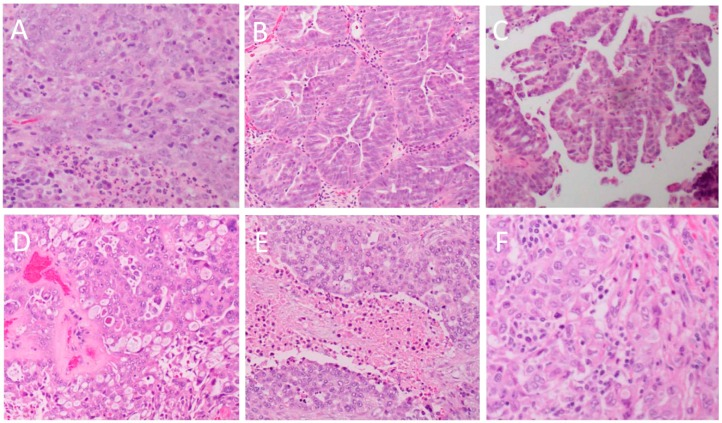
\includegraphics[width=\textwidth]{Introduction/Figs/Raster/ijms-20-00952-g001.jpg}
    \caption[Morphology types in HGSOC]{Heterogeneous morphology of HGSOC tissues, examples from Murakami \textit{et. al.}\citep{murakami2016establishment}. A) Solid growth architecture B) C) D) E). }
    \label{fig:morphology_murakami}
\end{figure}
\citep{murakami2016establishment, Lisio2019Feb}

\subsection{Collagen}
Collagen is the main component of the extracellular matrix, collagen deposition is a key part of desmoplasia. 

\subsection{Second-harmonic generation}

Second harmonic generation(SHG) is a nonlinear optical process in which two photons with the same frequency interact with a nonlinear material and combine to make a single new photon with twice the energy of the initial photons (half the wavelength). Collagen fibres are one such non-linear material and can be imaged using the SHG method. An advantage of this is that SHG imaging is marker free and so can be carried out without the requirement of antigen retrieval. 


%********************************** %Second Section  *************************************
\section{What drives HGSOC?} %Section - 1.2

TP53 mutations are believed to be ubiquitous in high grade serous. The HGSOC genome is extremely complex and highly rearranged. In the face of such complexity it is difficult to elucidate exactly what is causing what.  \citep{RN17}


\nomenclature[z-HGSOC]{HGSOC}{High Grade Serous Ovarian Cancer}
\nomenclature[z-TMA]{TMA}{Tissue Micro Array}
\nomenclature[z-IMC]{IMC}{Immuno Metal Conjugation}
\nomenclature[z-IHC]{IHC}{Immuno histo chemistry}
\nomenclature[z-IF]{IF}{Immunofluorescence}
\nomenclature[z-SHG]{SHG}{Second Harmonic Generation}
\nomenclature[z-GLCM]{GLCM}{Grey Level Co-occurence Matrix}


%!TEX root = ../thesis.tex
%*******************************************************************************
%*********************************** Methods chapter *****************************
%*******************************************************************************

\chapter{Methods}  %Methods

\ifpdf
    \graphicspath{{Methods/Figs/Raster/}{Methods/Figs/PDF/}{Methods/Figs/}}
\else
    \graphicspath{{Methods/Figs/Vector/}{Methods/Figs/}}
\fi


%********************************** %First Section  **************************************
\section{Patient Cohorts} %Section - 1.1 

Multiple patient cohorts were used throughout the thesis and are detailed at the beginning of the sections they are used in. 

\begin{itemize}
    \item SEARCH
    \item BRITROC
    \item OV04
    \item ICON7
\end{itemize}

\section{Chromogenic Immunohistochemistry (IHC)}

\subsection{Sample preparation}
3μm sections of FFPE blocks were cut using a Leica microtome, transferred to a water bath pre-heated to 60${^\circ}$C and collected on a glass slides. The sections were dried over-night at 37${^\circ}$C then baked at 60${^\circ}$C for 1h. 

\subsection{Manual Staining} 
\subsection{OV04/BRITROC}\label{sec:sarwah_staining}
FFPE sections were rehydrated using the Leica Autostainer ST020 by incubating them twice for 10 min in xylene, followed by two 5 min incubations in 100\% ethanol, one 5 min incubation in 70\% Ethanol and finally washing them in water. Antigens were retrieved in a Tris (10 mmol)-EDTA (1mM) buffer (pH 9.2) preheated to 96${^\circ}$C in a water bath. After 1h incubation, slides were cooled in a water bath for 5 min, washed in Milli-Q water for 5 min and incubated in3\%BSA-PBS for 1h in a hydration chamber at room temperature. ImmEdge pen was used to draw a hydrophobic border around the tissue, and 200μl of primary antibody pre-diluted to the desired concentration in 1\%BSA-PBS were added to the sections. Following an overnight incubation in a hydration chamber at 4$^{\circ}$C, the antibody solution was drained and the slides were washed twice for 5 min in 1\% Tween-TBS, succeeded by two washes for 5 min in TBS. For HRP-conjugated primary antibodies, DAB was directly added to the slides. For secondary antibody staining, pre-diluted secondary antibody was added and incubated at room temperature for 30 min, followed by 2 washes in TBS. The slides were incubated in DAB chromogen for
5 min, washed in Milli-Q water, and dehydrated and cover-slipped using the Leica Autostainer ST020.

\subsubsection{SEARCH}
Sectioning and was carried out as following on the SEARCH cohort. Microarray slides composed of FFPE embedded ovarian tumour cores were dewaxed and rehydrated prior to heat induced epitope retrieval (HIER) using a pressure cooker and a citrate-based antigen unmasking solution (Vector Laboratory). Detection of CD8$^+$ T cells, CD45RO$^+$ memory lymphocytes and CD68$^+$ macrophages was performed using the mouse anti-human CD8 (Clone C8/144B, Dako), mouse anti-human CD45RO (Clone UCLH, Dako) and mouse anti-human CD68 (Clone M0876, Dako) antibodies, using ultrasensitive Polymer-HRP IHC Detection system (Biogenex). Immunohistochemical protocols and slide hybridizations were carried out manually. Sections were counterstained with haematoxylin and mounted with DPX mounting medium (Sigma). Stained slides were scanned using the Panoramic Slash Scanner (3D Histech).

\subsection{Automated Staining}
Automated staining was carried out using the Ventana Discovery Ultra platform.  All bulk reagents used were purchased from Roche and are listed in Table \ref{table:bulk_reagents}. The slides were rehydrated by incubating them in EZ prep solution for 32 min at 69${^\circ}$C, then incubated for 1h in VentanaCell Conditioning buffer 1 (CC1) at 96${^\circ}$C for antigen retrieval (pH 8.5). Hydrogen peroxide was then applied and incubated for 4 min to quench endogenous peroxidase activity, followedby primary antibody incubation for 1h at 37${^\circ}$C. Details of antibodies used for chromogenic IHC are listed in Table \ref{table:ihc_antibodies}.  After a16 min incubation with an HRP-conjugated secondary antibody, the chromogenic signal was developed in either 3, 3’-Diaminobenzidine (DAB) chromogen for 8 min, in Purple chromogen for 40 min, in Yellow chromogen for 28 min or in Teal chromogen for 8 mins. For chromogenic counter-staining, the slides were incubated for 4 min in Copper,8 min in haematoxylin and 4 min in Bluing Reagent. Slides were washed with Reaction Buffer after each incubation. As a negative control, Mouse IgG, Rabbit IgG and GoatIgG isotype replaced mouse, rabbit and goat primary antibodies, respectively. Stained slides were dehydrated using the Leica Autostainer ST020, manually cover-slipped and digitally scanned by Aperio Scanscope XT. 
\begin{table}[]
    \centering
    \begin{tabular}{lc}
    \hline
    Reagent & Code \\
    \hline
    EZ prep & 950-102 \\
    Ultra Cell Conditioning Solution (CC1) & 950-224\\
    Ultra Liquid Cover Slip (LCS) & 650-210 \\
    Reaction Buffer & 950-300 \\
    ChromoMap DAB Kit & 760-159\\
    Purple Kit & 760-229 \\
    Yellow Kit & 760-239 \\
    Antibody Diluent & 760-108\\
    Haematoxylin II & 760-2208\\
    Bluing reagent & 760-2037\\
    OmniMap Anti-Ms-HRP Secondary Antibody    & 760-4310\\
    OmniMap Anti-Rb-HRP Secondary Antibody & 760-4311 \\
    \hline
    \end{tabular}
    \caption{Caption}
    \label{table:bulk_reagents}
\end{table}

\section{Imaging Mass Cytometry}
\subsection{Imaging Mass Cytometry (IMC) Antibody purification}
Carrier proteins like bovine serum albumin (BSA) are commonly added to the storage buffer of antibodies as preservatives. These proteins can replace antibodies in the conjugation process,reducing the efficiency of antibody conjugation to metals. Antibodies with carrier proteins were therefore purified using the Pierce™Antibody Clean-up Kit (ThermoFisher, 44600) following the manufacturers instruction.  This involves a desalting step, where the antibody is passed through a Zeba spin desalting column containing a resin bed and centrifuged for 2 min at 1000×g. The antibody is then added to a spin column containing a Purification Support slurry,incubated at room temperature for 5 min with end-to-end mixing, then centrifuged for 1 min at 4000×g to collect the purified antibody.The purity of the antibody was tested using a NuPAGE™4-12\% Bis-Tris Gel (Invitrogen,NP0321BOX). The antibody was mixed with LDS Sample buffer (Invitrogen, NP0007) and Sample Reducing agent (Invitrogen, NP0009) and incubated at 70${^\circ}$C for 10 min. 1μg of the original antibody and the purified antibody were loaded onto the gel, with a BSA-only sample used as a control. The gel was run in Bolt MPOS SDS Running Buffer (Invitrogen, B0001)at 120V for 30 min followed by 2h at 60V. The gel was stained with InstantBlue (Expedeon,ISB1L) to visualise the protein bands, and imaged using Antibody-Metal conjugation Carrier-free antibodies were metal-conjugated using the Maxpar®X8 Antibody Labelling Kits (Fluidigm) according to the manufacturers instructions. A proprietary polymer is loaded with a lanthanide metal by mixing them in the provided L-buffer and incubating them in a 37${^\circ}$C water bath for 35 min. The metal-loaded polymer is filtered to remove excess metal by centrifuging it twice in a 30kDa Amicon Ultra500 μlV bottom (Millipore, UFC505096) at 14,000×g for a total of 55 min. The antibody is centrifuged at 14,000×g in a 50kDa AmiconUltra500 μlV bottom (Millipore,  UFC505096) for 10 min,  and then partially reduced by incubating it in 4mM PierceTM Bond-Breaker®TCEP Solution (ThermoFisher Scientific,77720) at37${^\circ}$C for 30 min.  This is immediately followed by three washes in the provided C-buffer, with a 10 min centrifugation at 14,000×g after each wash. The metal-loaded polymer is added to the partially reduced antibody and incubated in a 37${^\circ}$C water bath for 90 min.The metal conjugated antibody is washed four times in the provided W-buffer, with a 10 min centrifugation at 14,000×g after each wash. The antibody is finally suspended in 100μl PBS containing 0.05\% sodium azide as a preservative, and collected by centrifuging the inverted filter in a fresh microcentrifuge tube for 2 min at 1,000×g. The concentration of the antibody was measure using NanoDrop Spectrophotometer ND-1000 (LabTech International).

\subsection{Staining and Imaging}
The manual staining  protocol outlined in  section \ref{sec:sarwah_staining} was also followed for IMC.  Metal-conjugated primary antibodies were used instead of unconjugated or HRP-conjugated antibodies. Details of all antibodies used are displayed in Table \ref{table:imc_antibodies}.
\begin{table}[]
    \centering
    \begin{tabular}{lllllc}
    \hline
    Antigen & Clone & Tag & Source & Code & Concentration() \\
    \hline
    CA9 & polyclonal & 141Pr & Novus & BioAF2188 & 2  \\
    p53 & DO-7 & 143Nd & Fluidigm & 3143026D & 5 \\
    CD16 & EPR16784 & 146Nd & Fluidigm & 3146020D & 10\\
    CD163 & EDHu-1 & 147Sm & Fluidigm & 3147021D & 5 \\
    PanK & C11 & 148Nd & Fluidigm & 3148020D & 1 \\
    CD56 & MRQ-42 & 151Eu & Cell Marque & 156R-96 & 1 \\
    CD45 & D9M8I & 152Sm & Fluidigm & 3152018D & 1.5\\
    LAG3 & D2G40 & 153Eu & Fluidigm & 3153028D & 2.5\\
    TIM3 & D5D5R & 154Sm & Fluidigm & 3154024D& 2.5\\
    FoxP3 & 236A/E7 & 155Gd & Fluidigm & 3155016D & 5\\
    CD4 & EPR6855  & 156Gd & Fluidigm & 3156033D & 5\\
    CD68 & KP-1 & 159Tb & Fluidigm & 3159035D & 2\\
    PD1  & D4W2J & 160Gd & Cell Signalling & 86163S & 5 \\
    CD20 & H1 & 161Dy & Fluidigm & 3161029D & 5\\
    CD8 & aC8/144B & 162Dy & Fluidigm & 3162034D & 5\\
    CD103 & EP206 & 163Dy & Cell Marque & 437R-16 & 3\\
    CK7 & RCK105 & 164Dy & Fluidigm & 3164028D & 10\\
    pH2AX & N1431 & 165Ho & Fluidigm & 3165036D & 0.5\\
    B7h4 & D1M8I & 166Er & CST14572 & 5 \\
    GranzymeB & EPR20129-217 & 167Er & Fluidigm & 3167021D & 1 \\
    Ki67 & B56 & 168Er & Fluidigm & 3168022D & 1.5\\
    Collagen 1 & Polyclonal & 169Tm & Fluidigm & 3169023D & 1\\
    CD3 & Polyclonal & 170Er & Fluidigm & 3170019D & 7.5\\
    CTLA4 & BSB88 & 171Yb & BioSB & BSB 2885 & 7.5\\
    OX40 & ACT-35 & 172Yb & CST98785 & 5\\
    CD45RO & UCHL1 & 173Yb & Fluidigm & 3173016D & 3\\
    HLADR & TAL 1B5 & 174Yb & ThermoFisher & MA1-46109  & 0.5\\
    ICOS & D1K2T & 175Lu & CST & 3148021D & 5\\
    Histone H3 & D1H2 & 176Yb & Fluidigm & 3176023D & 0.25\\
    Intercalator &  & 191Ir, 193Ir  & Fluidigm  & 201192A & 1:1000\\
    \hline
    \end{tabular}
    \caption{IMC antibodies}
    \label{table:imc_antibodies}
\end{table}
Following the two washes in 1\% Tween-TBS and two washes in TBS, the slides were counter-stained with Cell-ID™Intercalator-Ir for 30 min at room temperature. The slides were then washed in Milli-Q water for 5 min, and air dried for at least 20 min before imaging on the Hyperion™Imaging System(Fluidigm). Images were acquired using a UV laser at a frequency of 200 Hz. Metals in each pixel ablated were plasma-ionised and their count was detected using Cytometry by Time of Flight (CyTOF) technology. This was used to generate a stack of false-colour images, each layer corresponding to a single metal and the intensity of each pixel reflects the amount of each antigen present. 

\subsection{Image analysis}
Python was used for data cleaning and applying median filters.

Imagej was used for analysis of collagen structure.

QuPath was used for classification of individual cells from H&E and Cytokeratin images.

Definiens was used for the classification of SEARCH.  Definiens image analysis algorithms for detection of epithelial and stromal areas were trained and the segmentation for each core was manually refined by AM and a consultant gynaecological-histopathologist (J. McD.).

Analysis of images taken from both chromogenic IHC and IMC was done using the HALO Image Analysis Platform (Indica labs). Halo was used for tissue classification and immune cells identification and extraction in SEARCH, BRITROC and OV04. 

%********************************** % Fourth Section  *************************************
\section{Statistical Analysis}  %Section - 1.4
\label{section1.4}

R (version 3.5.1) was used for statistical analysis and R markdown documents are provided in Supplementary Methods that reproduce all results. All count data were transformed to log base 10 after adding a small offset to zero values. Wilcoxon signed rank test was used to compare the mean infiltrate between groups. Continuous data were presented as median and interquartile range (IQR) and groups were compared by the Kruskal–Wallis and pairwise Kruskal-Wallis tests. Discrete data were presented as count and percentage.  

The functional form of immune variables was assessed using comparison with cubic splines. The best approximations to the functional forms were carried forward for the Cox models. 

I carried out quality assurance tests for spatial bias across TMAs and investigated the sources of varying tissue area visually using heatmaps and statistically using Shapiro-Wilk tests.


\subsection{Survival Analysis}

Cox regression was used to examine the relationship between predictors $X$ and the hazard.

The hazard function is given by the following formula:
\begin{equation}H(t) = H_0(t) e^ {b_1 X_1 + ... + b_n X_n} \end{equation} 

Where $H$ is the hazard, the predictors are denoted $X_n$ and Cox regression estimates the coefficients of the predictors $b_n$. The proportional hazard model is semi-parametric as there is an assumption that the hazard is a linear function of the predictors and that the hazards are proportional (the coefficients are not a function of time). There are no assumptions about the form of the baseline hazard function $H_0(t)$. 

The Akaike Information Criterion (AIC), equation \ref{eq:AIC} as detailed in the Methods, was used to compare the performance of survival models, which includes the loglikelihood of the model $\hat{L}$ and a penalty on the number of terms, $k$ to reduce overfitting. 

\begin{equation}
\label{eq:AIC}
    {\displaystyle \mathrm {AIC} \,=\,2k-2\ln({\hat {L}})}
\end{equation}

\subsection{Spatial Statistics}

Spatial statistics can most easily be carried upon 2D point patterns. In such analyses cells are assumed to be points with coordinates $(x,y)$ and zero radius $r=0$. The value of the center of the point for each cell is given in equation \ref{eq:1}. 

\begin{equation}    x=\frac{x_{max} + x_{min}}{2}        y = \frac{y_{max} + y_{min}}{2}
\label{eq:1}
\end{equation}
We will see that these assumptions are violated but information can still be gleaned from these measurements as long as the consequences and limitations of such assumptions are understood.

The spatial patterns of a distribution can be split into first order properties (density variation) and second order properties (how points influence the location of others).

\subsection{Density based analysis}

\subsubsection{Global density}
The simplest measure of the density of a point pattern is the following:
\begin{equation}
    \lambda = \frac{n}{|A|}
\end{equation}
Where $\lambda$ is the number of points in a region and $A$ is the area measure of the region. 

\subsubsection{Ripley's K function}
Ripley's K function measures the distribution of points within a certain radius and is defined as:
\begin{equation}
K(r)=\lambda^{-1}E
\end{equation}
Where $\lambda$ is the density and $E$ is the expected number of points in the region.

\subsubsection{DBSCAN}
DBSCAN stands for Density based clustering. There are many clustering methods in existence but when clustering spatial data rather than data in information space, DBSCAN has been shown to be best at clustering groups\cite{}.

\subsubsection{Getis Ord Hotspot Analysis}
Getis Ord hotspot analysis assesses whether the density of events (eg. immune cells) is higher in a subregion than on average in the region overall. 

The Z score for such a region is 
\begin{equation}
    z_i = \sum_{j=1}^{n}w_{i,j}c_{j} - \frac{\bar{c}\sum_{j=1}^{n}w_{i,j}}{SU}
\end{equation}

where S and U are given by the following:

\begin{equation}
    S = \sqrt{\frac{\sum_{j=1}^{n}c_{j}^2}{n} - (\bar{c})^2 }
\end{equation}

\begin{equation}
    U = \sqrt{\frac{n\sum_{j=1}^{n}w_{i,j}^2 - (\sum^n_{j=1}w_{i,j})^2}{n-1} }
\end{equation}


\subsection{Distance based analysis}
\subsubsection{Average Nearest Neighbour}
This analysis measures the average distance from each point to its nearest neighbouring point. 

\subsubsection{k-nearest neighbour}
k-nearest neighbour method derives for each point in a point pattern, the $k^{th}$ nearest neighbour to it.
The theoretical expected distance \ref{eq:knn} to the nearest neighbour in a random 2D point pattern is derived as follows;

\begin{equation}

\end{equation}

\begin{equation}
\label{eq:knn}
    <r_n> = \frac{1}{2\sqrt{\lambda}}
\end{equation}
Where $\lambda$ is the global density of points.

\subsubsection{Pair Correlation function}

The $g$ function sums the number of points within a narrow distance band.

\subsection{Intensity analysis}

The Grey Level Co-occurence Matrix (GLCM)\cite{GLCM} measures texture features based on second order statistics based upon pixel intensities.


$P_{ij}$ is the $i,j$ element of the normalized GLCM. $\mu$ is the mean of the GLCM.

The statistics that are commonly calculated on the GLCM\cite{haralick1973textural} include the following:

\subsubsection{Entropy}
Entropy is a measure of information mixing. Increasing disorder increases entropy. Shannon entropy is defined as \begin{equation}
    H = -\sum_{i=1} {p_i log p_i}
\end{equation}

Where $p_i$ is the probability of obtaining class $p$.

Entropy can be defined on an image or image region based on pixel grayscale values.

In the GLCM notation, entropy is:

\begin{equation}
    \mathrm{Entropy} = -\sum_{i,j=0}^{N-1} P_{ij} ln{P_{i,j}}
\end{equation}

\subsubsection{Energy}
Sum of squared elements in the GLCM. 
\begin{equation}
    \sum^{N-1}_{i,j=0}(P_{ij}^2)
\end{equation}


\subsubsection{Contrast}
Local variation in intensity, measuring the difference in neighbouring pixel values. \begin{equation}
    \sum^{N-1}_{i,j=0}P_{i,j}(i-j)^2)
\end{equation}

\subsubsection{Homogeneity}
This measures the tightness of the distribution of pixels values.
\begin{equation}
    \sum^{N-1}_{i,j=0} \frac{P_{i,j}}{1+(i-j)^2}
\end{equation}

\subsubsection{Correlation}
This measures the correlation between neighbouring pixels, a perfectly correlated image would have correlation = 1. 
\begin{equation}
    \sum^{N-1}_{i,j=0} P_{ij} \frac{(i-\mu)(j-\mu)}{\sigma^2}
\end{equation}


%!TEX root = ../thesis.tex
%*******************************************************************************
%****************************** Second Chapter *********************************
%*******************************************************************************

\chapter{Digital pathology and the quantification of immune infiltrate}

\ifpdf
    \graphicspath{{Chapter2/Figs/Raster/}{Chapter2/Figs/PDF/}{Chapter2/Figs/}}
\else
    \graphicspath{{Chapter2/Figs/Vector/}{Chapter2/Figs/}}
\fi

\section[Introduction]{Introduction}
Immune infiltration is frequently manually assessed in pathology departments. Digital pathology is not yet routine in the clinic but increasingly part of modern research as more digital imaging and quantification methods become available. 
Continuous data offers a large number of possibilities for analysis and across the literature there are many approaches. The majority of papers have focused on quantifying epithelial infiltrate alone. Regardless, tissue specific infiltrate requires segmenting the epithelial and stromal compartments and the identification of cells by thresholding for nuclei based on a nuclear stain. The stromal and epithelial immune infiltrate in a tissue section can then be quantified.  In this chapter I worked to complete simple analyses on a dataset from the SEARCH cohort that contained the density of CD$8^+$, CD45RO$^+$ and CD68$^+$ immune cells in epithelium and stroma for each patient and aimed to develop a robust statistical workflow for the analysis of quantitative digital pathology data. I could then expand upon this basic analysis myself and ask questions about model building, the relative importance of stromal and epithelial infiltration, the relationships between them. I aimed to fully investigate, compare and interpret quantities of infiltration in different tissue regions in order to build up a better idea of the compartmental nature of the immune response.

\section{Collaborator Roles}
Anne Montfort (AM) - Sample Sectioning, Staining, Image segmentation\\
JMcD - Pathologist, Image segmentation\\
Anna Piskorz - Sequencing\\
Sarwah Al-Khalidi (SAK) - Resequencing of some samples\\

\subsection{History of the project}
This particular part of the work began from collaboration with AM who approached me with raw files from Definiens image analysis software of CD8$^+$, CD68$^+$ and CD45RO$^+$ stained slides, requiring data cleaning and manipulation and a basic analysis of the relationship between cell count density and survival. 

In this part of the PhD, I utilised this data set to build upon the foundational analysis that I carried out. Firstly investigating the TMAs for bias, extracting and examining the cores that were outlying in size or infiltration. I investigated the distribution of the infiltration densities and normalised them in order to use the correct statistical tests. Along with extracting and modelling the link between immune cell density and survival, I investigated more complex model building. I analysed varying functional forms of infiltrate density, combined multiple infiltrates with principal component analysis for the first time to investigate the underlying patterns of biology and did further analyses including quantifying and assessing the immune exclusion in samples. I also applied some similar analyses to the other subtypes of Ovarian Cancer in the cohort.

\begin{figure}
    \centering
    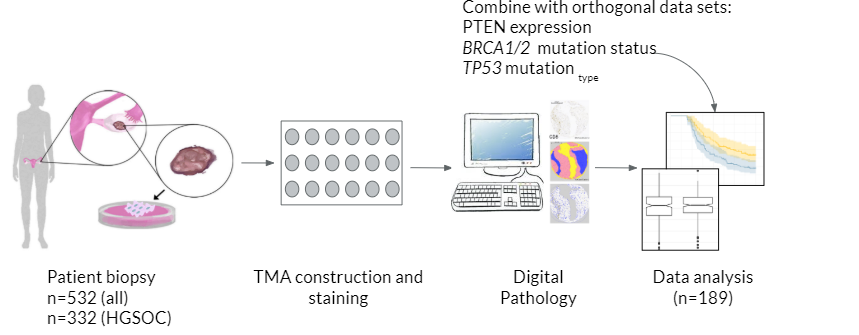
\includegraphics{Chapter2/Figs/Raster/Thesis_visual_abstract.PNG}
    \caption[Visual Abstract]{Visual abstract}
    \label{fig:visual_abstract}
\end{figure}

\section{SEARCH Cohort}

Samples from 570 patients from the prospective SEARCH ovarian cancer population-based study had been used to construct tissue microarrays. Ethical approval was granted by the Eastern Multicenter Research Ethics Committee. Among the samples from 570 patients with primary epithelial ovarian tumours, 332 were high grade serous ovarian cancer patients. All cases underwent detailed histopathological review by a gynaecological pathologist (JM). Patients were staged as having localized, regional or distant disease (L/R/D).

\section[Methods]{Methodology}
\subsection{SEARCH Data Set}
As mentioned, the immunohistochemical staining and initial utilization of Definiens software was carried out by AM. The methodology used to acquire the data set used in this section is outlined below and referred to in detail in the Methods chapter. 

\subsubsection{Immunohistochemistry}
Immunohistochemistry on the SEARCH samples was carried out upon the tissue sections by Anne Montfort (AM) according to the protocol in section \ref{sec:am_method}. Previously published PTEN immunostaining data was used where high PTEN expression was considered to be positive staining and low expression to be weak, heterogeneous or negative staining respectively\cite{RN17}.

\subsubsection{\texit{TP53} mutation data}

Sequencing and mutation analysis was carried out prior to this PhD by Anna Piskorz (AP). The coding regions of \textit{TP53} were sequenced by tagged-amplicon next generation sequencing (TamSeq) as previously described\cite{RN18} and confirmed by immunohistochemical analysis using a 4-tier core system\cite{RN19}. Sequencing of germline mutations in the  \texit{BRCA1} and \texit{BRCA2} genes was performed as previously described\cite{RN20}. Some samples were resequenced using TamSeq by SAK following my initial exploratory analysis and datacleaning steps. The results of resequencing were integrated into the final analysis.

\subsubsection{Immune cell quantification}
 The number of CD8$^+$ and CD45RO$^+$ cells in epithelial and stroma areas, the area of epithelial and stromal areas covered by CD68 staining and the total area of epithelium and stroma in each core, had been digitally determined using the Tissue Studio software (Definiens™).

Figure \ref{fig:segmentation} shows examples of this cell segmentation and tissue classification.

\begin{figure}[htbp!] 
\centering    
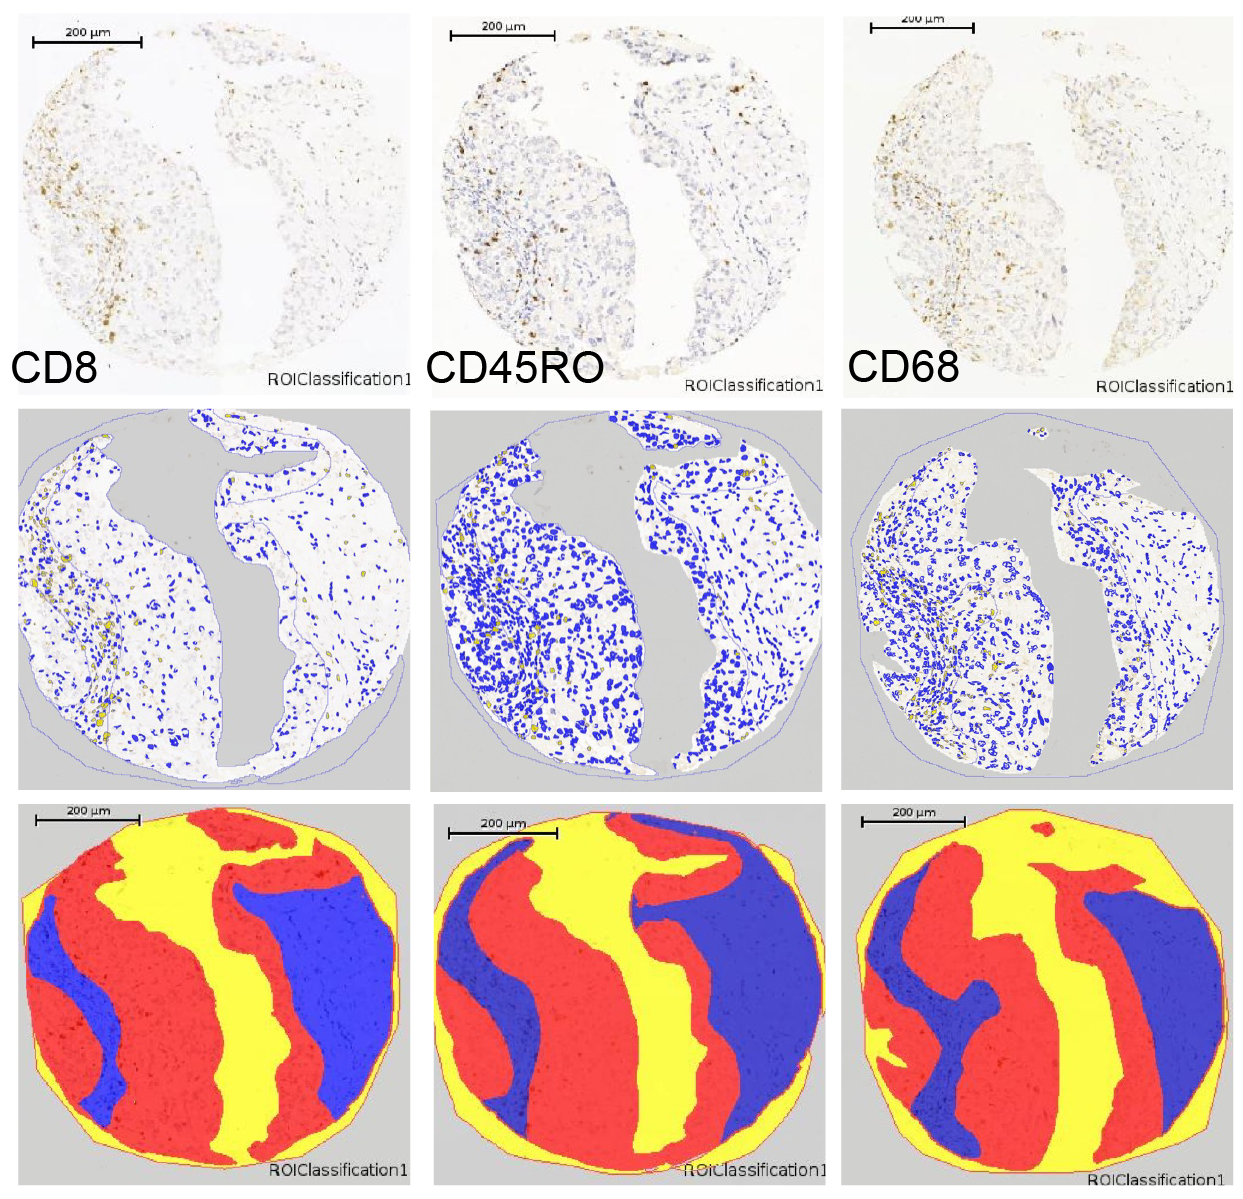
\includegraphics[width=0.8\textwidth]{Chapter2/Figs/Raster/Segmentation.png}
\caption[Segmentation in Definiens]{Examples of the segmentation of tissues and identification of cells in the Definiens software.}
\label{fig:segmentation}
\end{figure}

\subsection{Statistical analyses}
 The clinical variables of age at diagnosis, menopause status and stage were available for the cohort and I included them in the analysis. I used univariable Cox regressions to identify best-fitting variables for the final multivariable Cox regression model. The refined model was compared with a combined multivariable Cox regression model including all immune infiltrates. Hazard ratios (HR) refer to a single unit increase in continuous variables. The proportional hazards assumption was tested and satisfied in all cases using Schoenfeld residuals. The Kaplan–Meier analysis (with log-rank test) was applied to illustrate survival differences graphically. Two-sided P-values <0.05 were used to indicate statistical significance. 

Principal component analysis (PCA) using the R package \textbf{prcomp} was used to extract the independent components of variance between patients. The package \textbf{prcomp} uses singular value decomposition and the variables were scaled to have unit variance before creating composite linear independent variables. These were then passed forward to the survival modelling. The Akaike Information Criterion (AIC), equation \ref{eq:AIC} was used to compare the performance of survival models.

Bonferroni p-value corrections were carried out for all multiple testing. P < 0.05 was considered significant for all analyses. 


\section{Results}
 
 The SEARCH cohort included patients with HGSOC, Clear Cell, Endometrioid, Mucinous and Low Grade Serous Ovarian Cancer. These subtypes of Ovarian Cancer have vastly different cells of origin, different patterns of infiltration and different genomic drivers. As I was primarily interested in understanding the differences within populations rather than across subtypes, I extracted the HGSOC subpopulation for the initial analysis.

\subsection{Patient characteristics}
Figure {\ref{fig:remark_search}} shows the REMARK diagram for this study and Table \ref{table:clinical_SEARCH} shows the clinical characteristics of the 332 HGSOC patients from the study cohort. Immunohistochemical analyses on tissue microarrays (TMAs) were performed to detect CD8$^+$, CD45RO$^+$ and CD68$^+$ cells in tissue cores from primary ovarian specimens.  152 HGSOC cases were available for analysis after quality assurance, data cleaning and the reduction of the data set to only cases with complete results for CD8, CD45RO and CD68 staining in both epithelium and stroma as well as survival data. 
Tagged amplicon sequencing data was available for 248 cases and \textit{TP53} mutation was detected in 231 samples (93\%) (Table \ref{tab:clinical_SEARCH}). Previously published data for germline  \texit{BRCA1} and \texit{BRCA2} mutation and PTEN expression were available for 297 and 155 cases respectively\cite{17,20}.

\begin{figure}
    \centering
    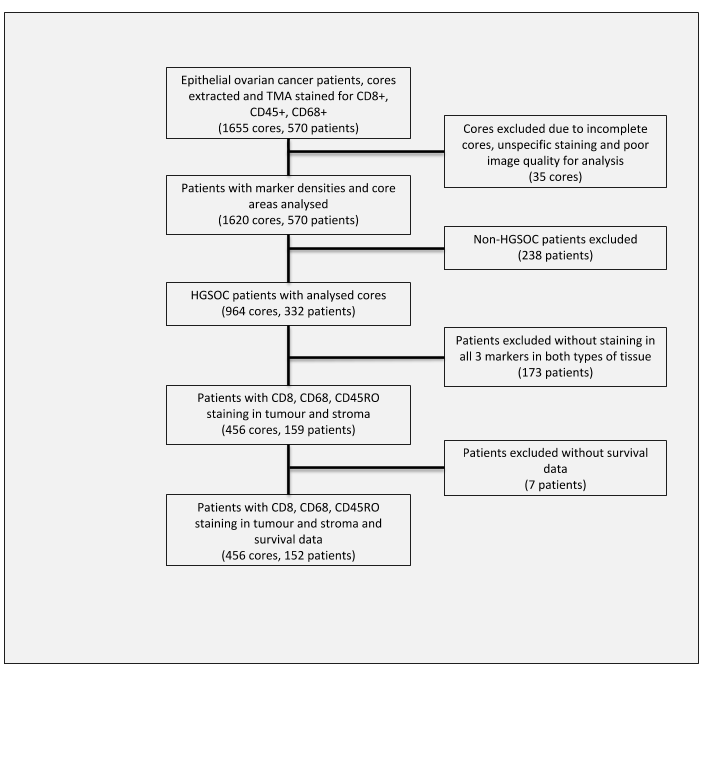
\includegraphics[width=0.8\textwidth]{Chapter2/Figs/Raster/montfort-REMARK.png}
    \caption{REMARK diagram for the SEARCH cohort.}
    \label{fig:remark_search}
\end{figure}
\begin{table}[]
    \centering
    \begin{tabular}{lll}
    \hline
 N	&	& 332 \\
Median Age (IQR) & & 58.0 (51.0-64.0) \\
\hline
Stage &	localized &	64 (19.3\%)\\
 &	regional &	42 (12.7\%)\\
 &	distant	& 202 (60.8\%)\\
 &	unstaged &	24 (7.2\%)\\
 \hline
TP53 mutation &	gof &	137 (55.2\%) \\
 &	lof &	94 (37.9\%)\\
&	wild type &	17 (6.9\%)\\
 &	Not assessed &	84 \\
 \hline
PTEN IF	& 	High &	28 (18.1\%)\\
& 	Low	 & 127 (81.9\%)\\
&	Not available &	177 \\
\hline
BRCA status		& 	wild type &	256 (86.2\%)\\
 &	\textit{BRCA1} &	18 (6.1\%)\\
 &	\texit{BRCA2} &	23 (7.7\%)\\
 &	Not available &	35\\
\hline
    \end{tabular}
    \caption{Patient characteristics for the HGSOC subset of the SEARCH cohort.}
    \label{tab:clinical_SEARCH}
\end{table}

 \subsection{Data cleaning, quality assurance and spatial bias}

Analysing a large number of digitally imaged and segmented TMA cores gave me the ability to carry out quality checking for bias across TMAs and to evaluate the variation in properties of the tissue core such as tissue area, something typically not measured by pathologists when assessing cores manually.

I examined the distribution of tissue area and ensured that the varying tissue area across TMAs was random \ref{fig:area_dist}. I did this visually using heatmaps (Figure \ref{fig:heatmap_area}) and statistically using Shapiro-Wilk tests ($p > 0.05 $). 

\begin{figure}
    \centering
    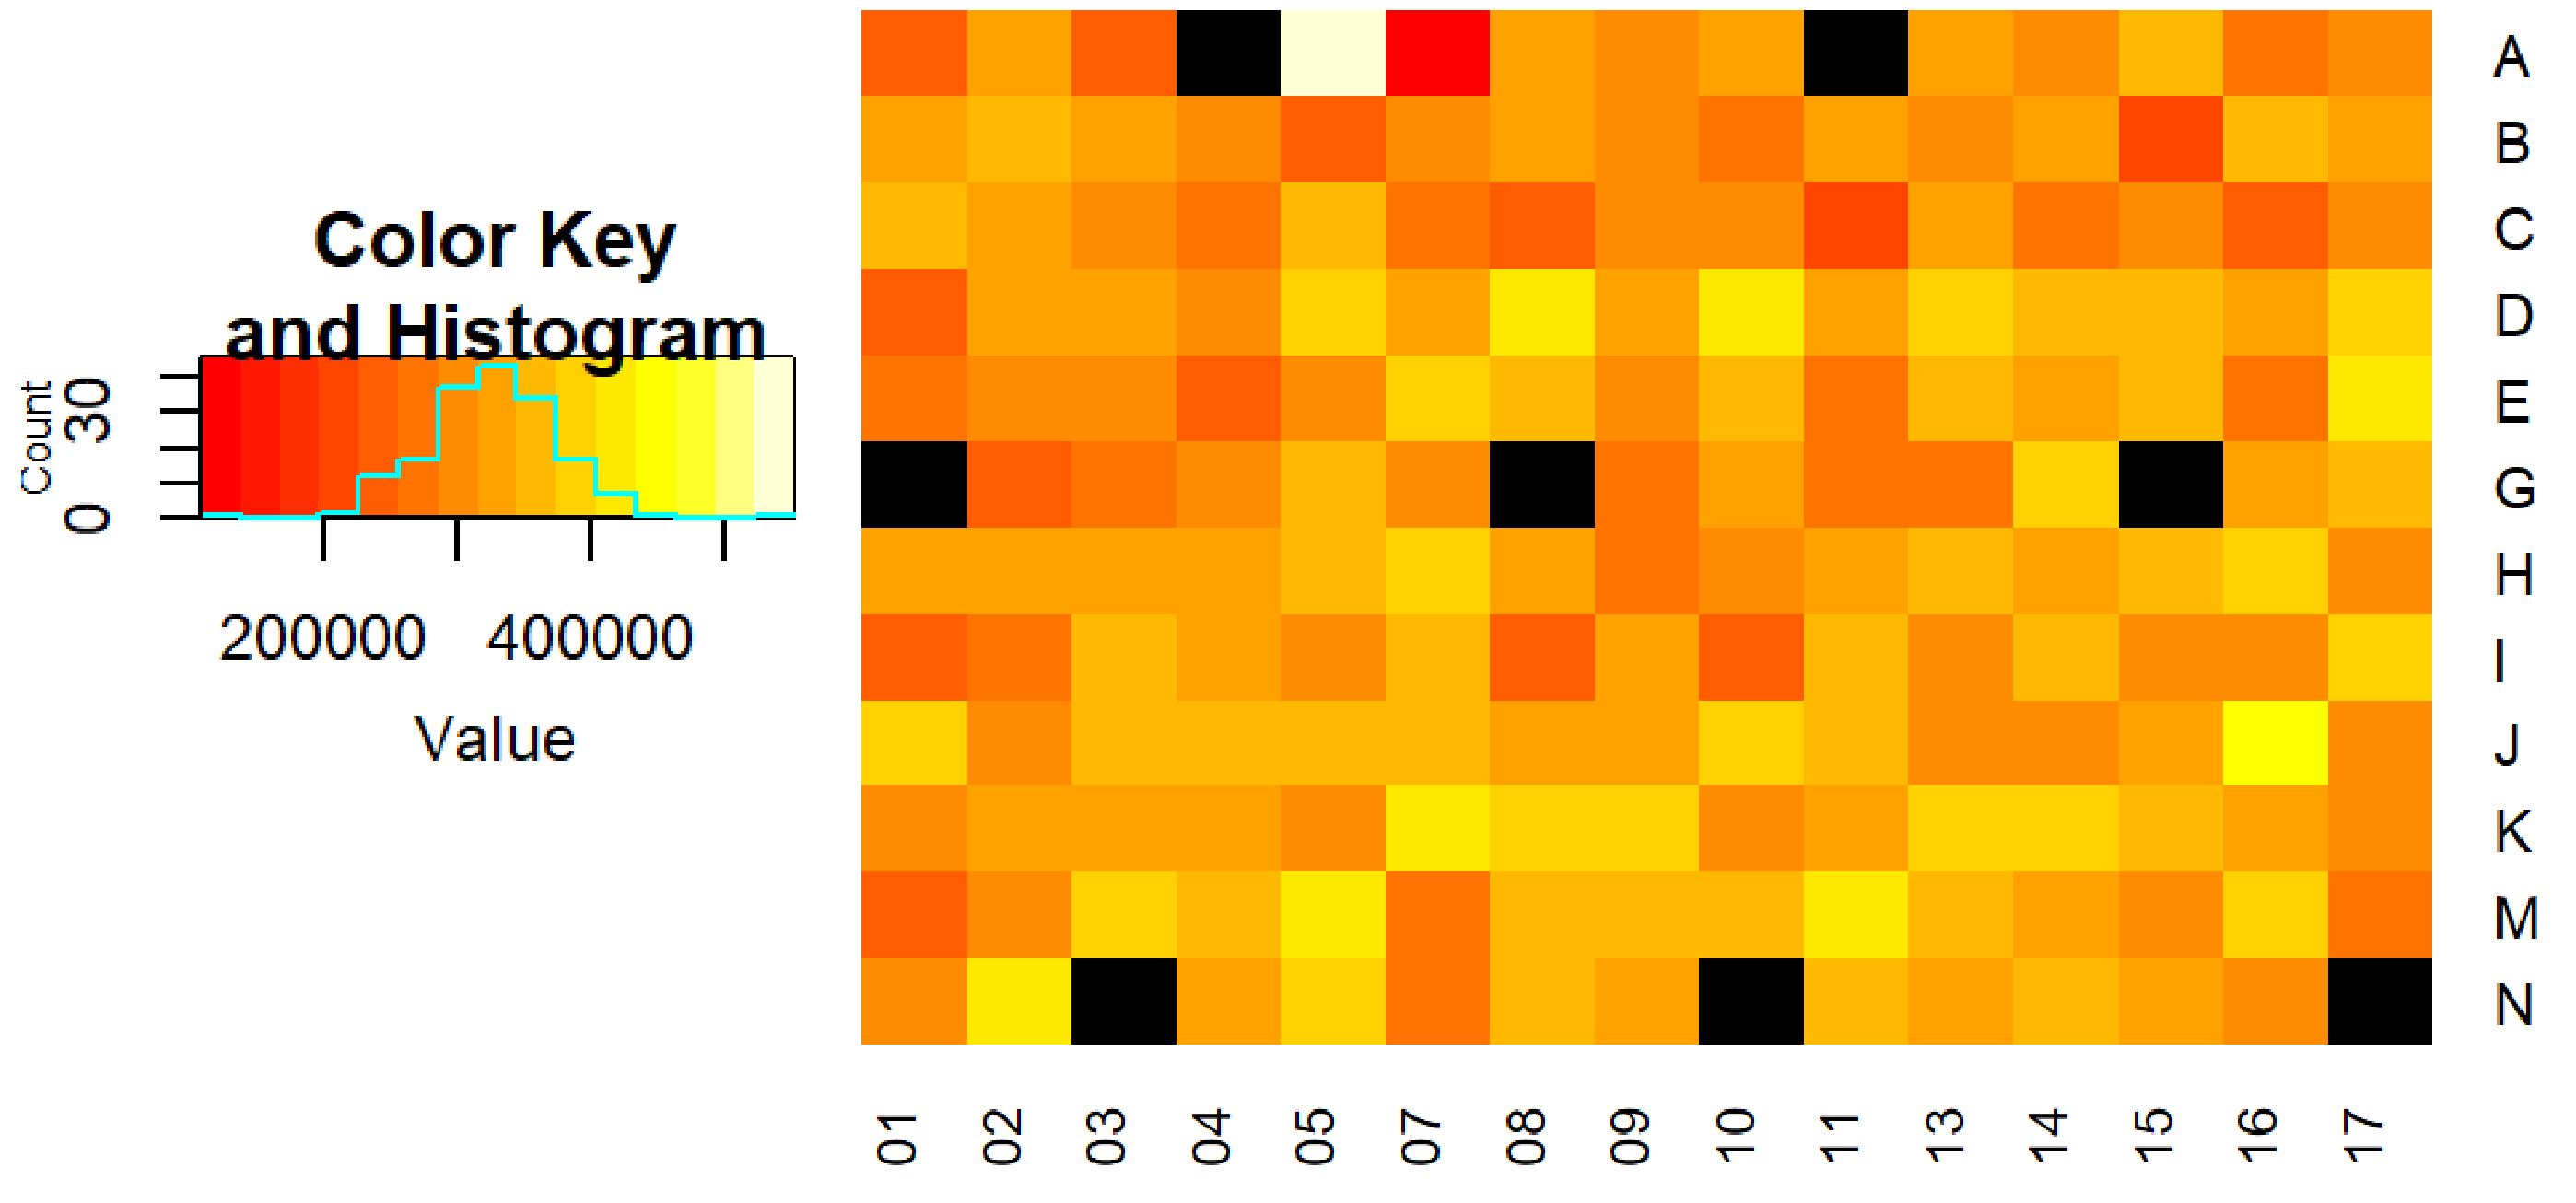
\includegraphics[width=0.8\textwidth]{Chapter2/Figs/Raster/area_heatmap.png}
    \caption{Heatmap of total core area across TMA.}
    \label{fig:heatmap_area}
\end{figure}

\begin{figure}
    \centering
    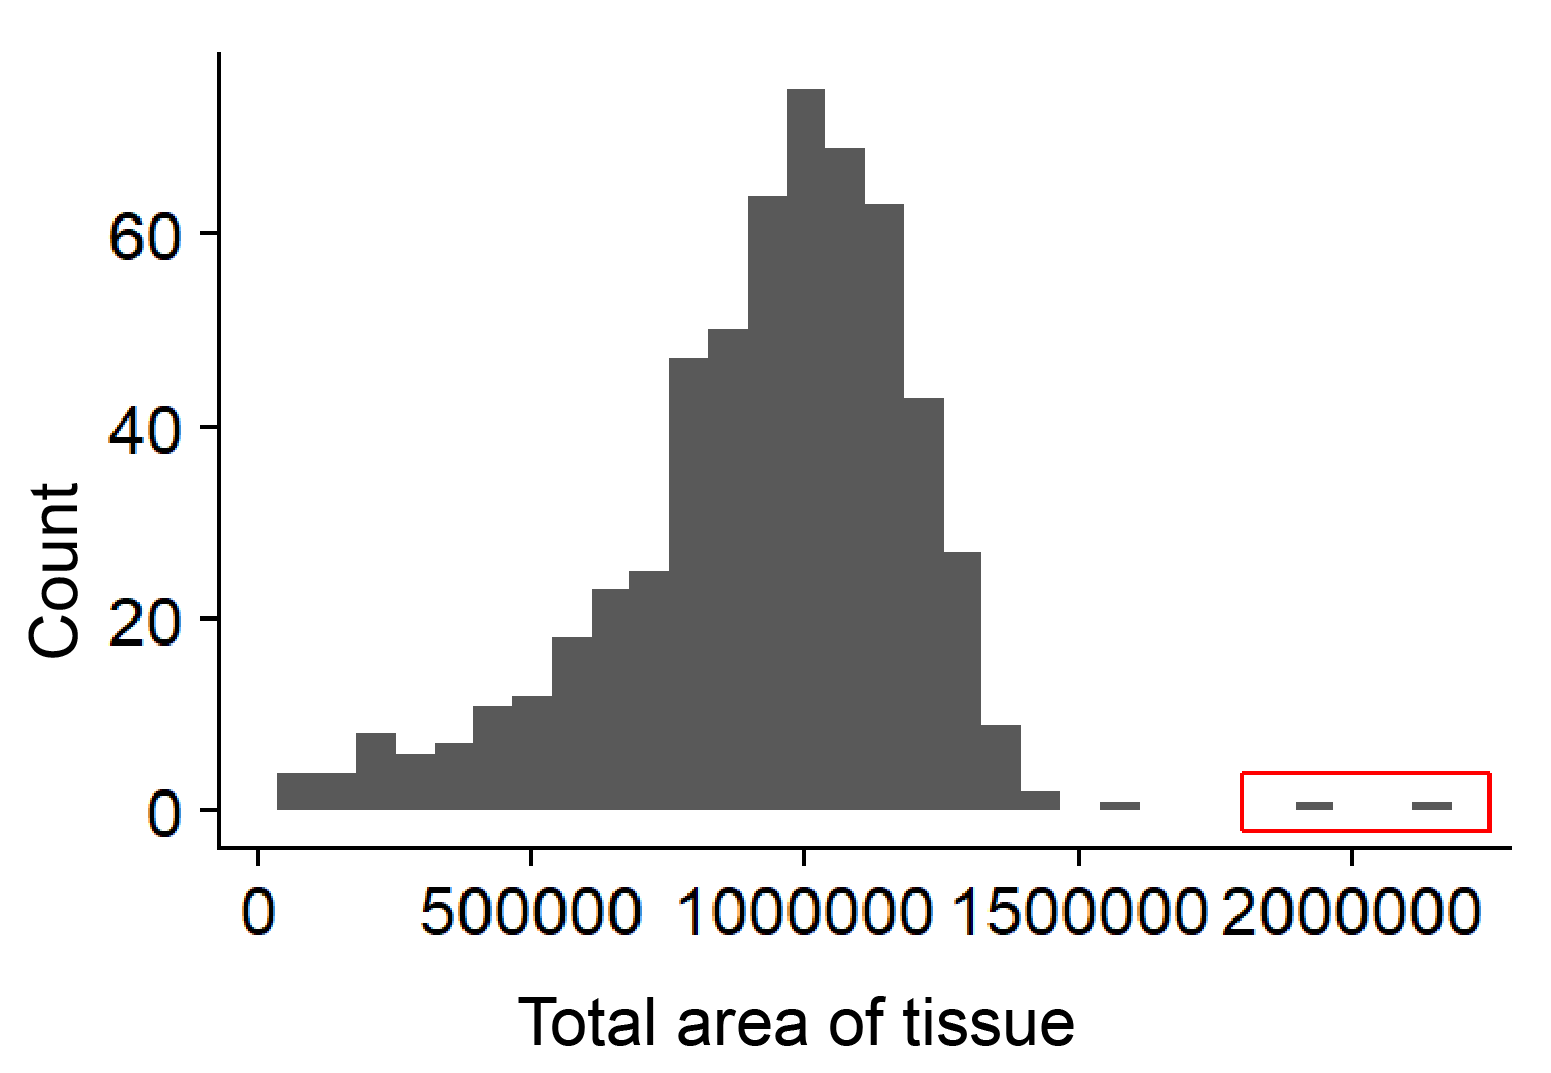
\includegraphics[width=0.4\textwidth]{Chapter2/Figs/Raster/Area_distribution_hist.png}
    \caption{The distribution of total tissue area for each core in the SEARCH cohort.}
    \label{fig:area_dist}
\end{figure}
 
As mentioned, CD8$^+$ and CD45RO$^+$ counts were initially calculated as number of cells in stroma and epithelium and CD68$^+$ scoring was given as area covered. I processed this raw data, converting cell counts into cells per unit area and CD68$^+$ coverage into percentage area. This normalization to area allows for comparison between patients whose tissue is made up of varying quantities of stroma and epithelium. I also confirmed using  residuals that transforming the count densities to base 10 would normalize them.


I also extracted outlying examples of cores to ensure the despite the tissue area sampled varying, that the measures of infiltrate density were not significantly different from the population as a whole. Figure \ref{fig:heatmap} shows a heatmap comparing infiltration density across the CD8$^+$ , CD68$^+$ and CD45RO$^+$ TMAs. No spatial relationship was observed over a single TMA between the location of a core and the density of immune cells or the tissue area. 



\begin{figure}
    \centering
    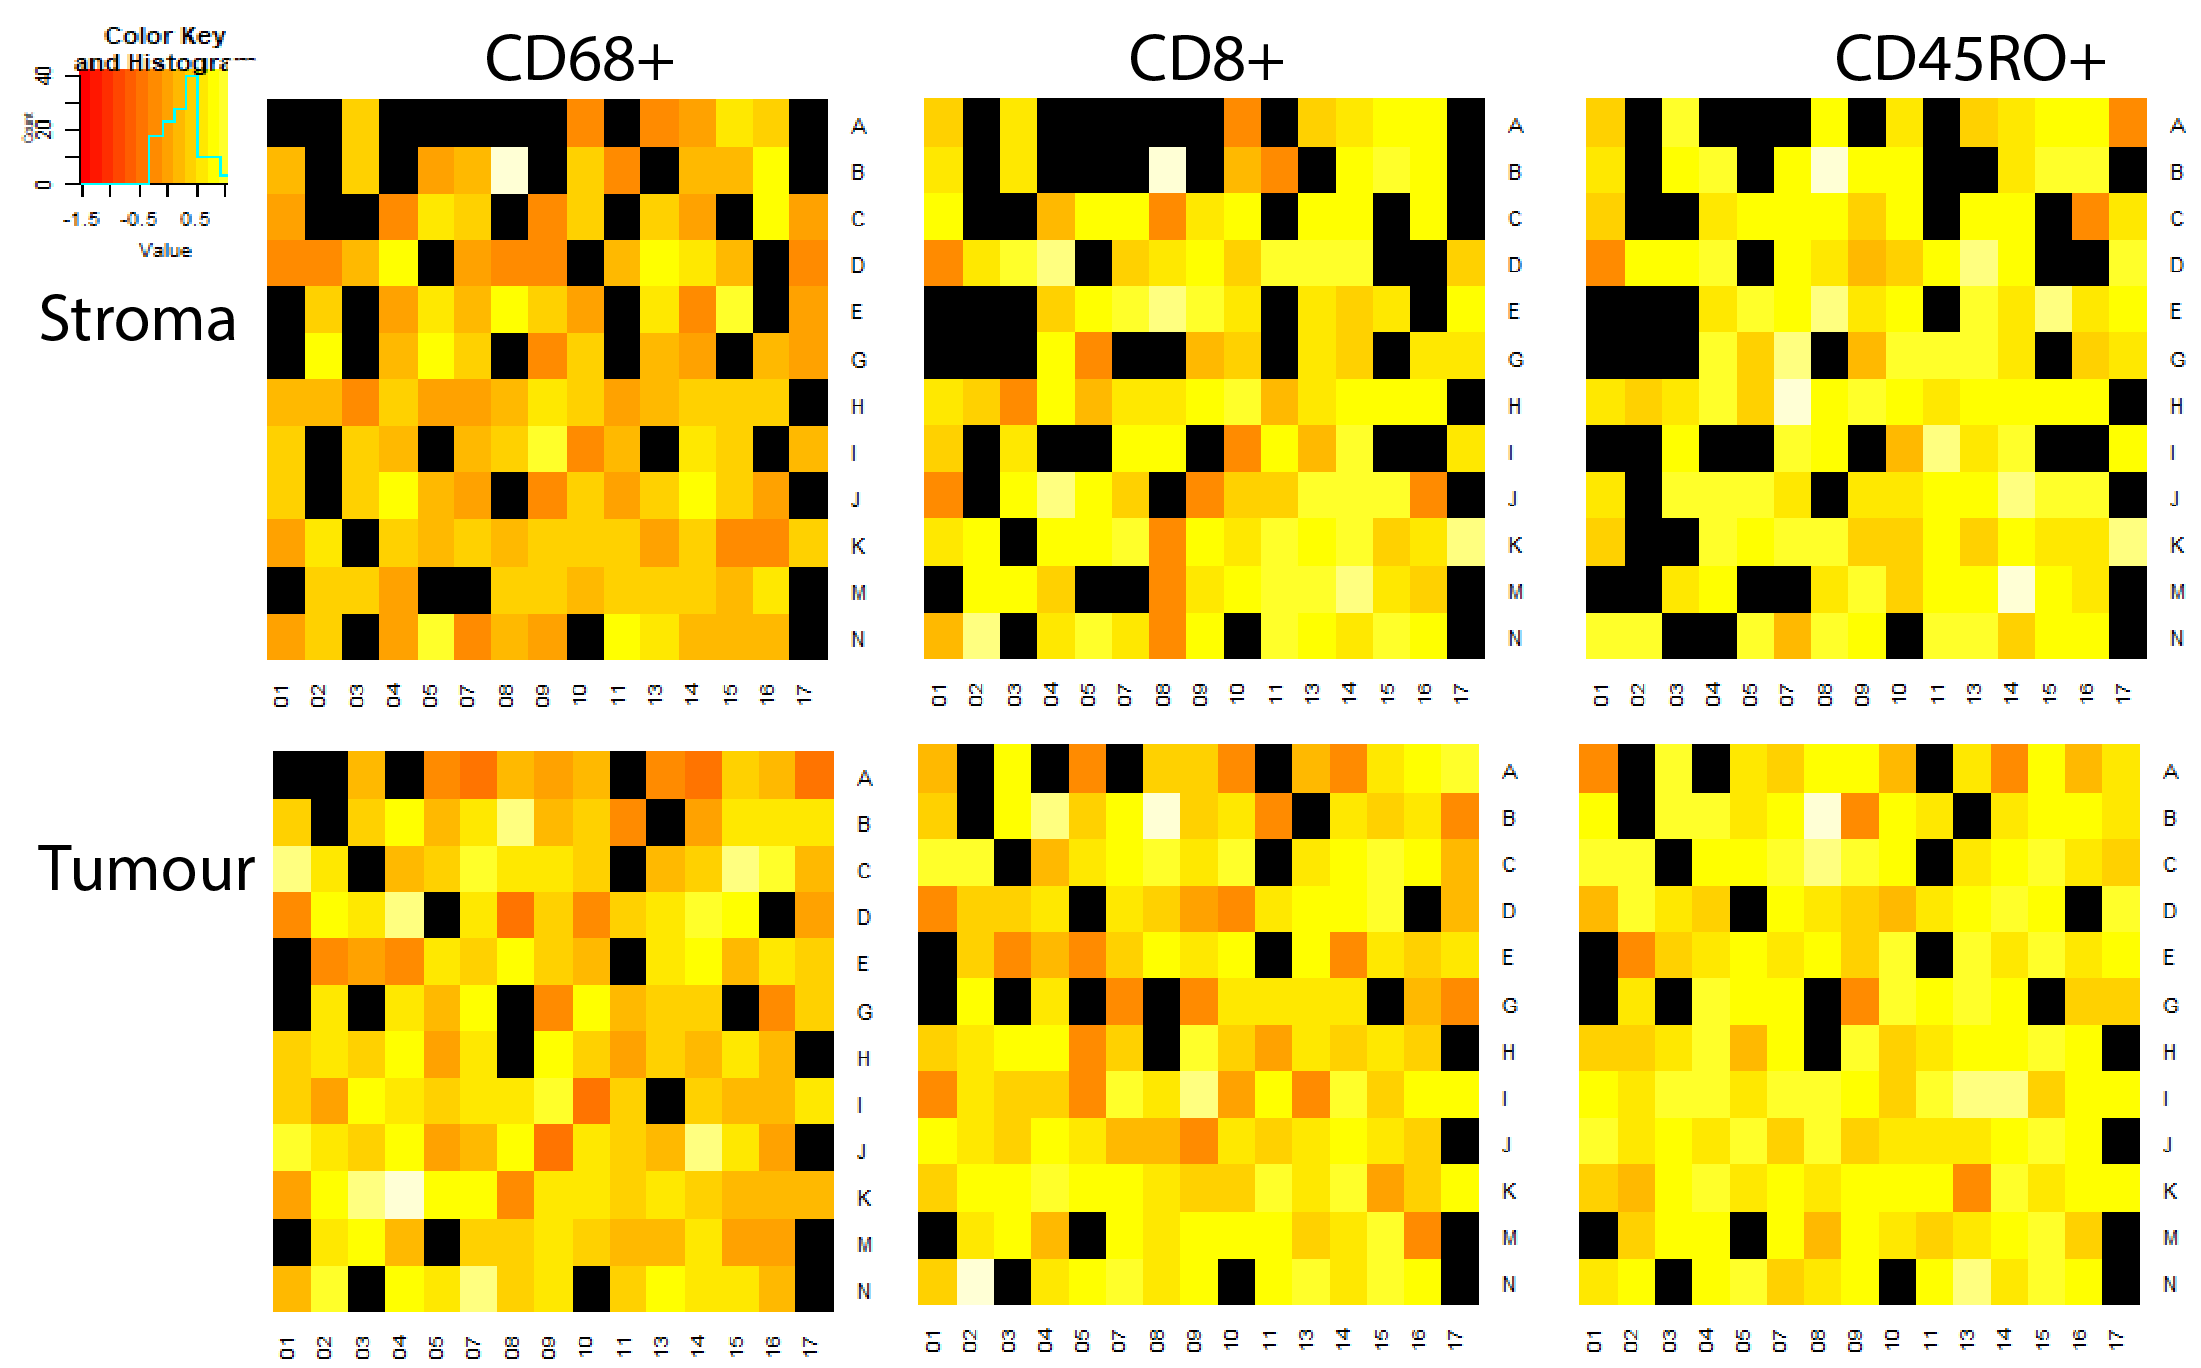
\includegraphics{Chapter2/Figs/Raster/Thesis-heatmap.png}
    \caption{Density of each infiltrate for each position in the SEARCH TMA.}
    \label{fig:outlying_core}
\end{figure}


\subsection{Stroma and tumour composition of cores}
Digital pathology and tissue segmentation provides a unique opportunity to evaluate stromal and epithelial areas and the makeup of sampled tissue cores. An example of the segmentation used to generate this data set is shown in Figure \ref{fig:segmentation}.  Pathologists sample tissue from sections of FFPE blocks for the construction of TMAs. Other than aiming to sample regions with high percentages of epithelium, this sampling is otherwise uncontrolled. I wanted to investigate the variation in epithelial and stromal tissue that was sampled in the SEARCH TMAs. The distribution of epithelial and stromal areas are shown in Figure \ref{fig:distribution_infiltrate}. \\

\begin{figure}
    \centering
    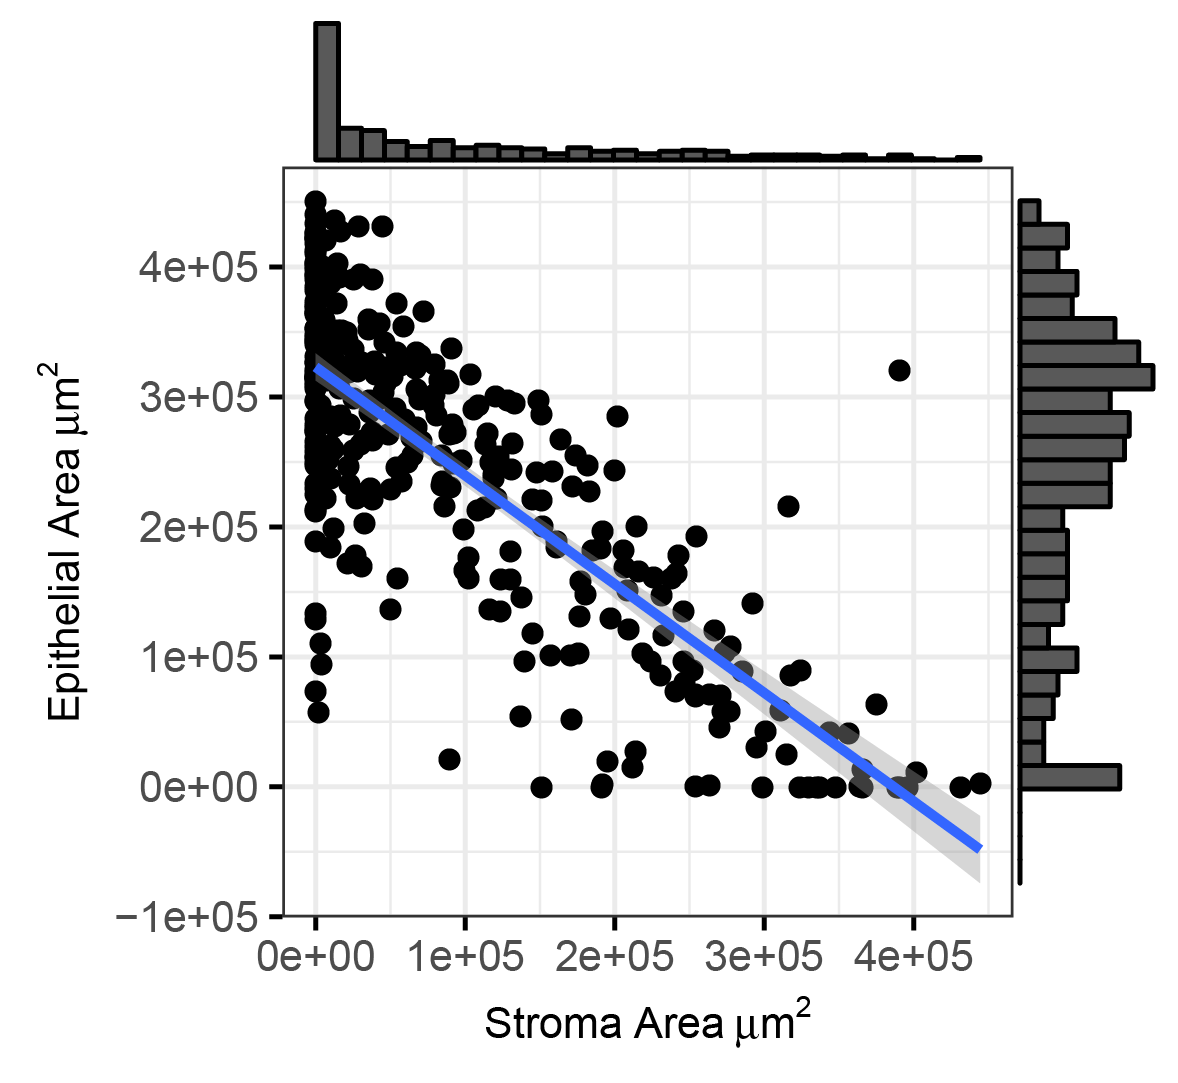
\includegraphics{Chapter2/Figs/Raster/Montfort-2018_epi_stroma_dist.png}
    \caption{The distribution of epithelial and stromal areas.}
    \label{fig:distribution_infiltrate}
\end{figure}

I found that of 964 images representing 332 HGSOC patients, 69 patients (20.8\%) had images which contained malignant epithelium but no stroma; 250 patients (75.3\%) had images which contained epithelium and >1\% adjacent stroma and 13 patients (3.9\%) had images containing no tumour epithelium (Fig \ref{fig:distribution_infiltrate}). The median proportion of epithelium and stroma was 85.1\% (IQR 51–100\%) and 14.9\% (IQR 0–49\%) respectively.

\subsection{Mutant allele fraction and epithelial content}

In order to perform a quality check on cores I utilised the side data set from this cohort of the mutant allele fraction for all samples. The distribution of mutant allele fraction is plotted as a histogram in  Figure \ref{fig:maf_dist}. I used this to ensure that the sequencing of all samples classified as HGSOC was of high enough quality. Samples with mutant allele fraction of zero were resequenced and if no mutation was found were excluded from HGSOC analysis.
\begin{figure}
    \centering
    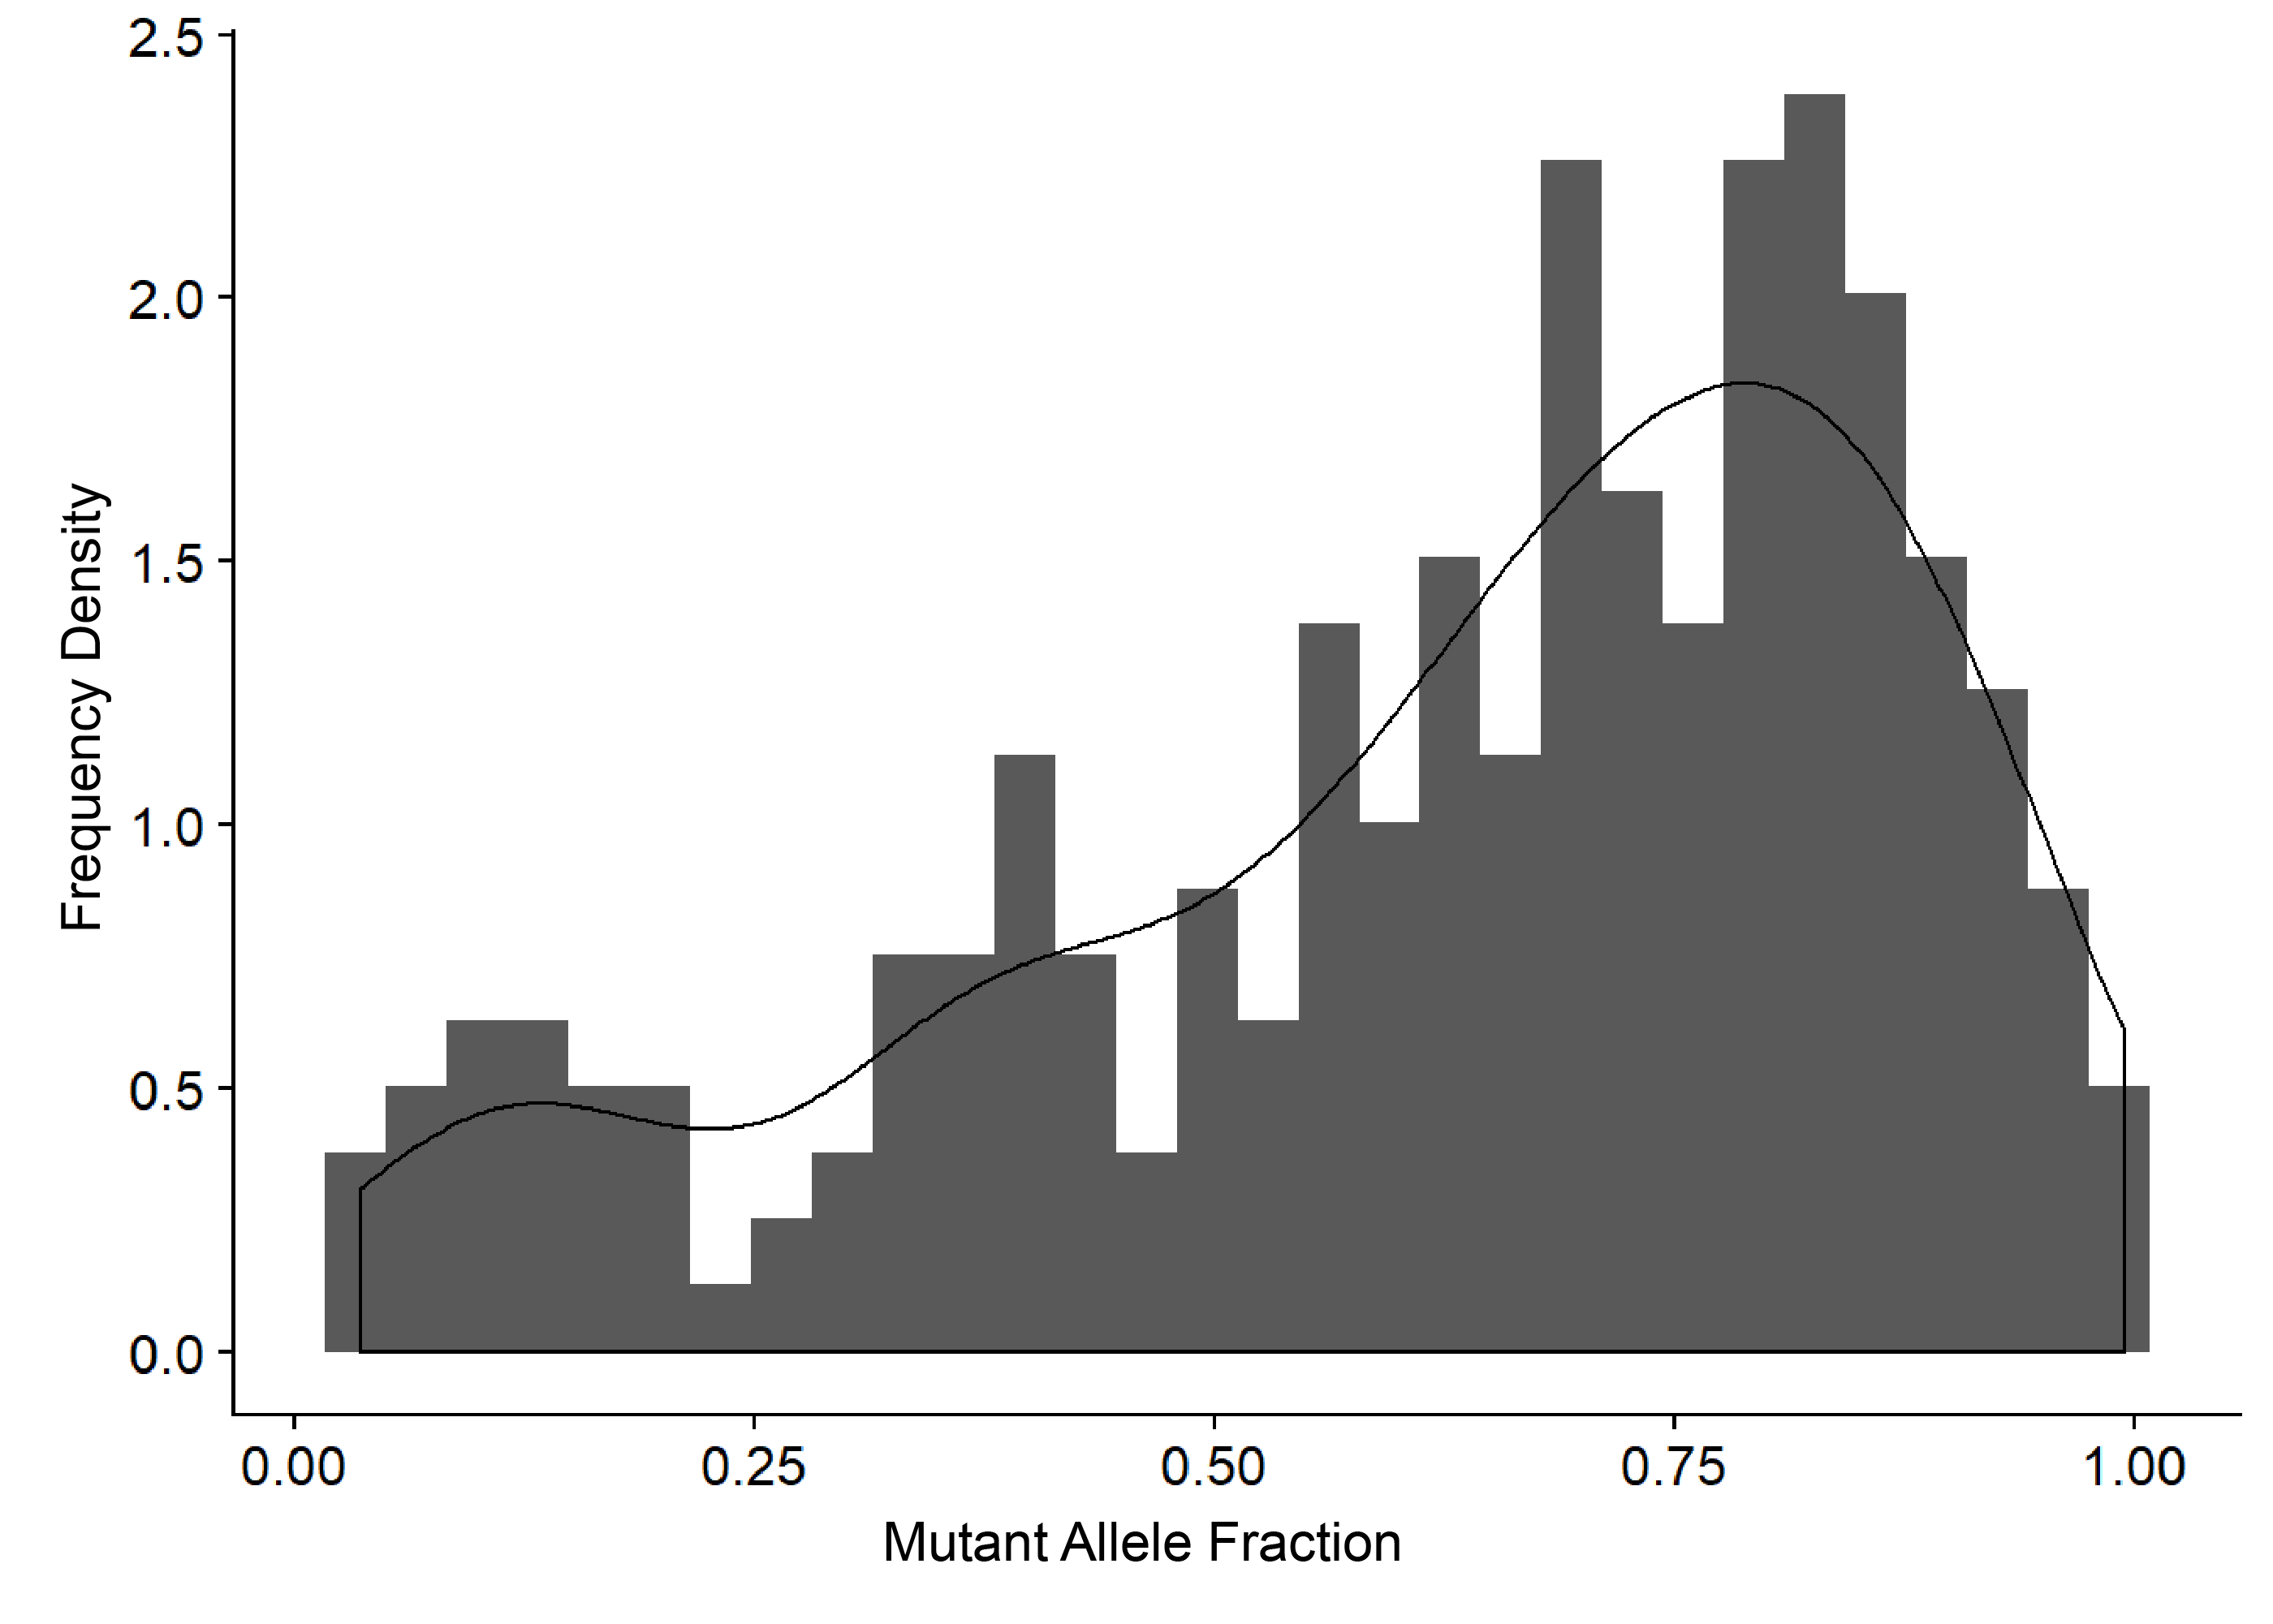
\includegraphics[width=0.4\textwidth]{Chapter2/Figs/Raster/MAF_distribution.png}
    \caption{Histogram of counts of samples against mutant allele fraction.}
    \label{fig:maf_dist}
\end{figure}

 As p53 mutations are found ubiquitously in HGSOC we would expect that the proportion of epithelial cells in a sample is correlated with \textit{tp53} mutant allele fraction.  I found them to be positively correlated ($R= 0.24$, $p=0.0027$). The sequencing and imaging are not carried out on exactly the same tumour region and so I would not expect a perfect correlation due to natural noise from sampling. The correlation between technical replicates for allele frequency and sequencing depth is shown in Appendix \ref{fig:p53_allele}. 
\begin{figure}
    \centering
    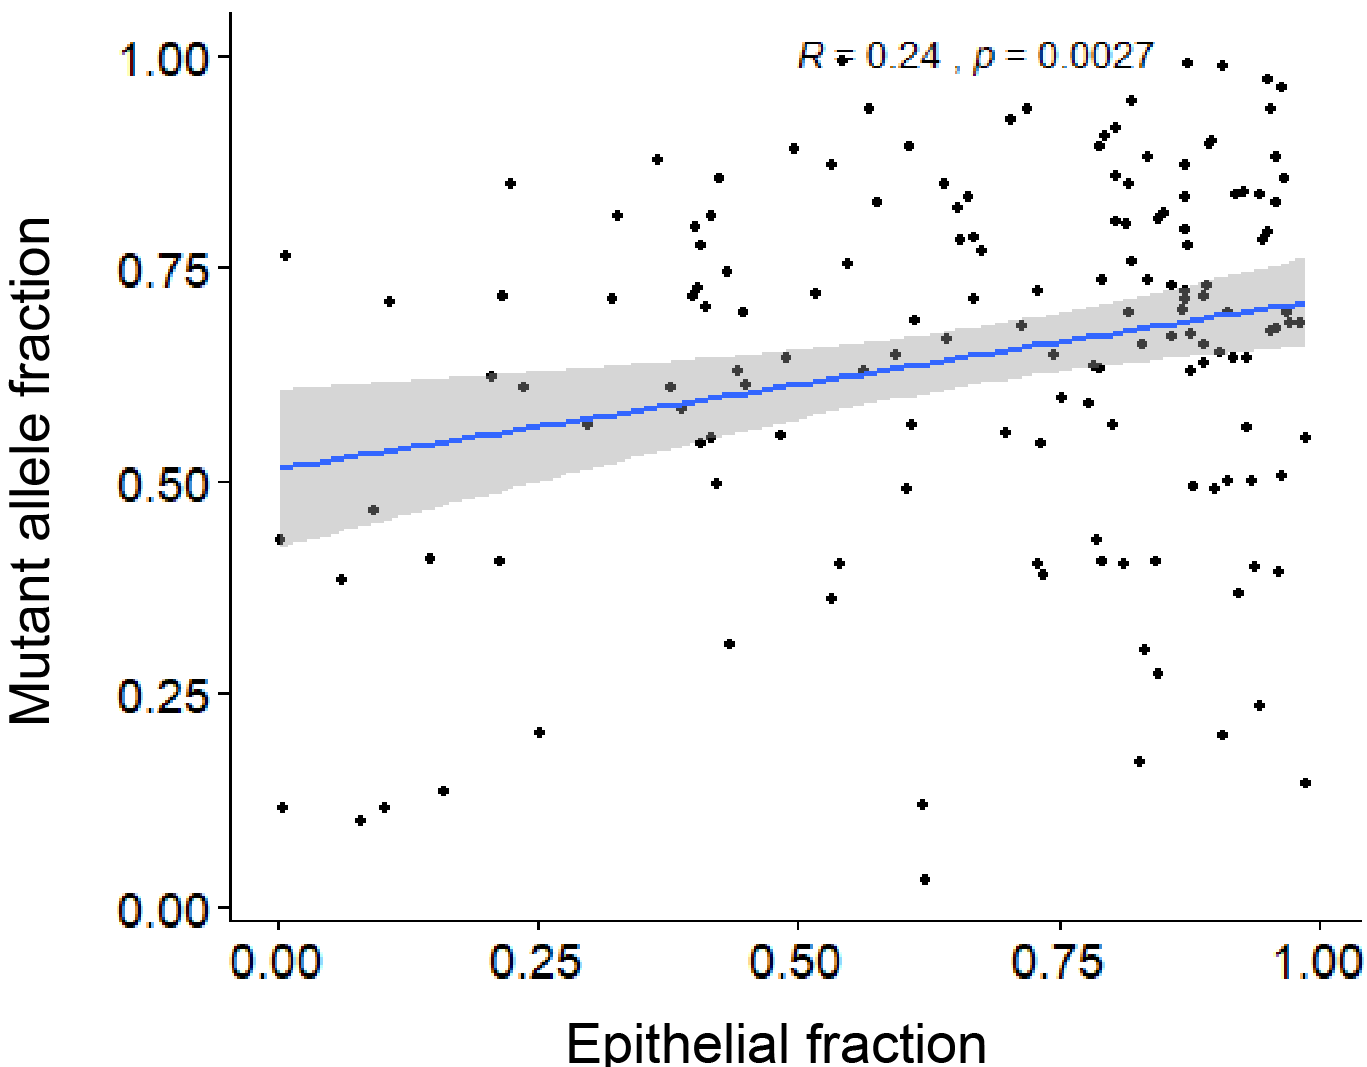
\includegraphics{Chapter2/Figs/Raster/maf_epithelial.png}
    \caption{\textit{p53} mutant allele fraction against epithelial area of a core.}
    \label{fig:p53_allele}
\end{figure}




\subsection{Immune cell densities}

An example of the assessment of CD8$^+$ T cell, CD45RO$^+$ memory lymphocyte and CD68$^+$ macrophage densities and the allocation of the stromal and epithelial regions is shown in Fig. \ref{fig:segmentation}.

As demonstrated, cores frequently sample varying areas of epithelium and stroma and therefore sample different proportions of epithelial and stromal infiltrate. In order to understand the impact of this sampling I felt that it was important to know how the density of infiltration varies between epithelial and stromal compartments. The distribution of densities of immune populations within tumour epithelium and stromal areas were compared (Fig. \ref{fig:distribution_infiltrate}). I found that the density of CD8$^+$ and CD45RO$^+$ cells were significantly higher in stroma than tumour epithelium (p = 0.005 and p = 0.004 respectively; Welch’s t-test) but not significantly different for CD68$^+$ cells. 

\begin{figure}
    \centering
    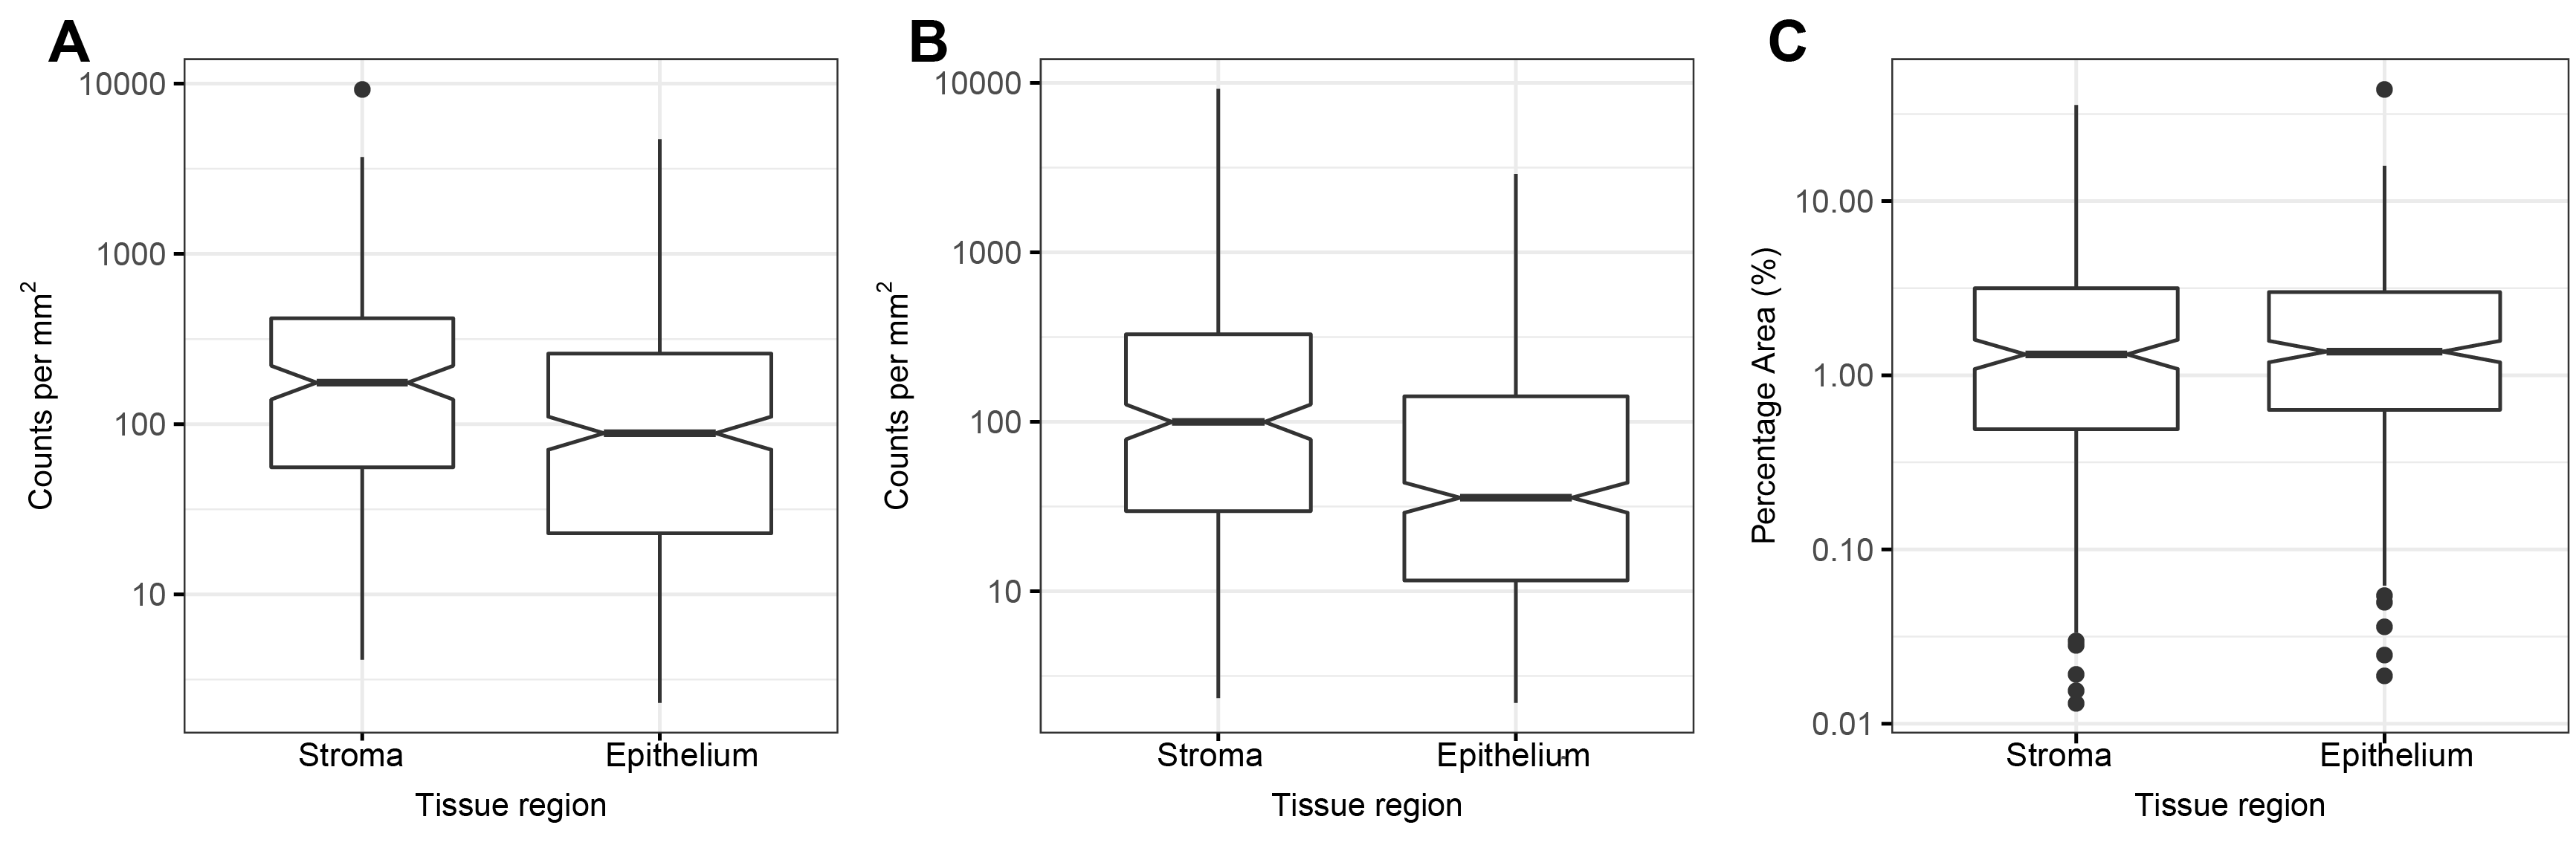
\includegraphics[width=\textwidth]{Chapter2/Figs/Raster/Montfort-2018_immune_Composition.png}
    \caption[Distribution of immune densities.]{ (A), (B) and (C) show the distribution of CD8$^+$, CD45RO$^+$ and CD68$^+$ immune cell densities in epithelium and stroma. CD8$^+$ and CD45RO$^+$ densities were defined as counts per mm2 and CD68$^+$ as the percentage of tissue stained for this marker. (Notches on box plots extend 1.58 ✕ IQR / sqrt(n) and approximate the 95\% confidence interval for the median. Box plot whiskers extend to 1.5 ✕ IQR.) 
}
    \label{fig:distribution_infiltrate}
\end{figure}

The predominant population of immune cells studied in the literature is epithelial CD8$^+$ infiltrate which has been demonstrated to have a log-linear relationship with survival. In order to evaluate the true nature of this infiltration in the microenvironmental context I investigated whether this infiltrate was independent of others. If this infiltrate is not independent, the survival impact may be an indirect readout of the presence of other infiltrates. The correlation between infiltrates is also important to understand whether there exist spatial dynamics of infiltration and the relationship and movement between adjacent tissue compartments. The quantitative measure of immune density in our samples allowed me to investigate the pearson correlation between quantities of immune infiltrate. The quantity of the three immune populations in this cohort showed moderate to strong correlation between infiltrate in epithelium and stroma and between the three infiltrates (Figure \ref{fig:ch2_correlation} and Table \ref{tab:cor_pvals}). 

\begin{figure}
    \centering
    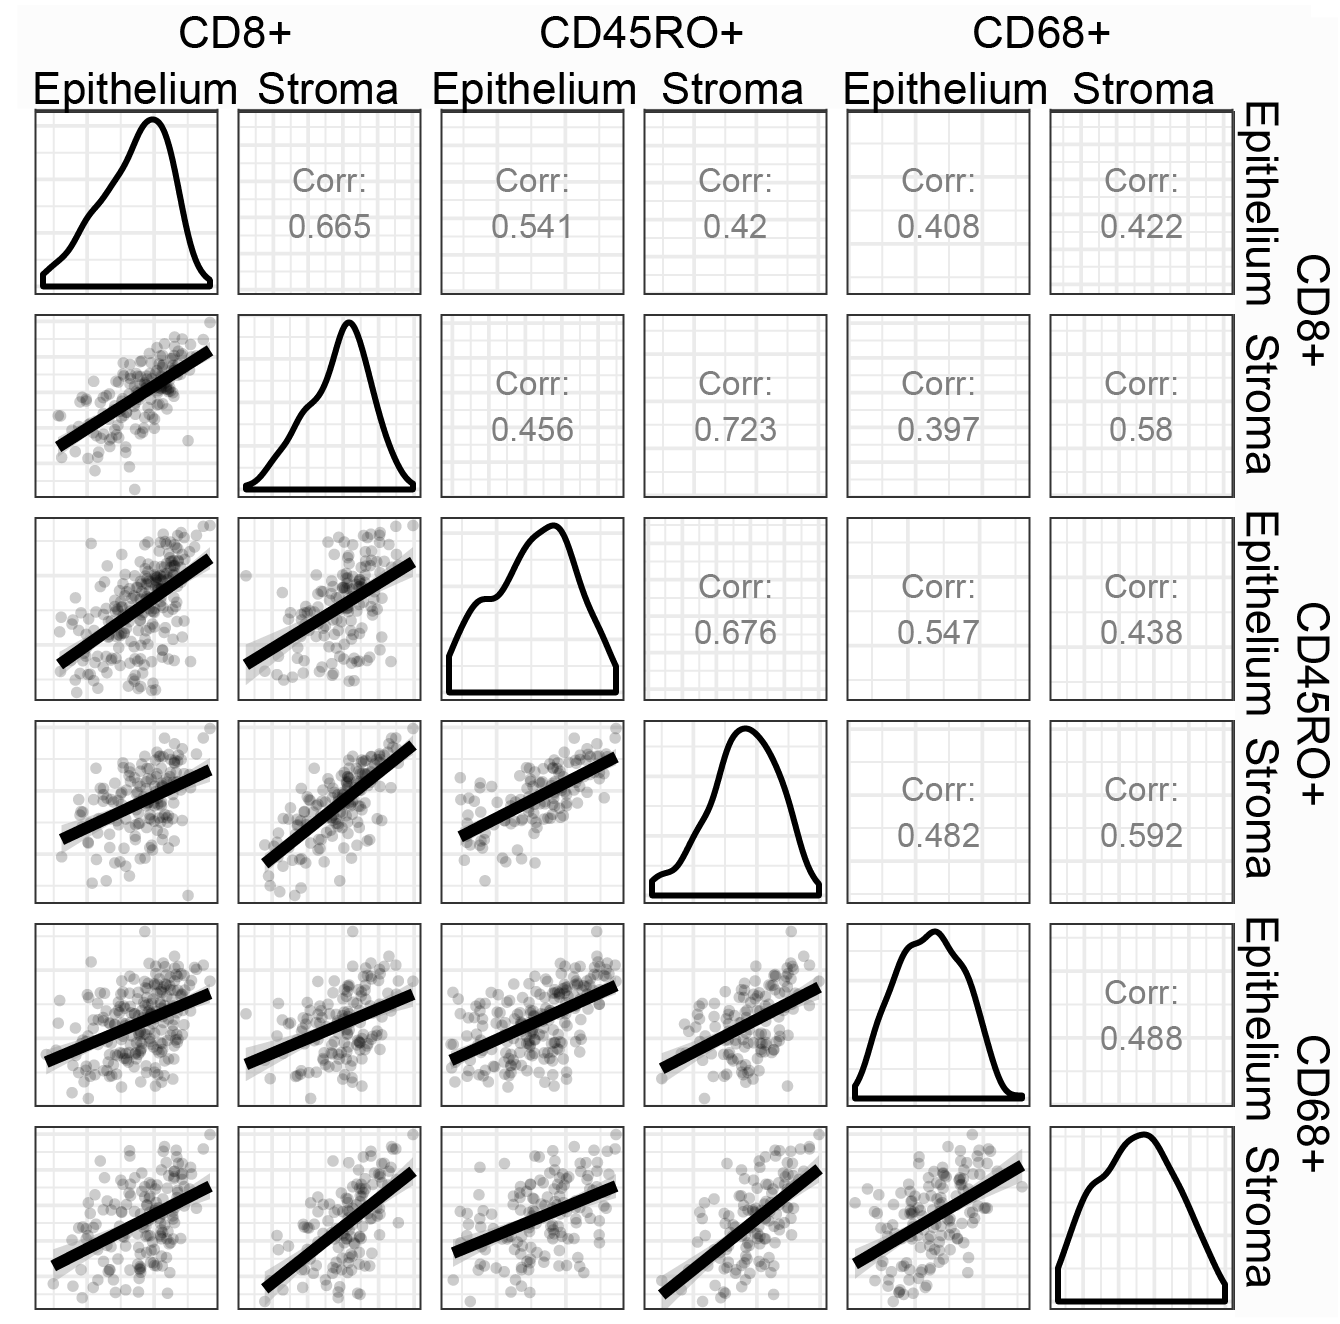
\includegraphics[width=0.8\textwidth]{Chapter2/Figs/Raster/correlation_inf.png}
    \caption[Correlation between infiltrates]{Scatterplots and distributions of CD68$^+$, CD45RO$^+$ and CD8$^+$ infiltrate in Stroma and Epithelium. The quantities of all infiltrates were correlated between matched samples across both tissue region classes.}
    \label{fig:ch2_correlation}
\end{figure}

Given that we see varying epithelial cell percentages and increased infiltrate in the stroma as compared with the tumour I was interested in whether the density of immune infiltrate reaching the epithelium was related to the epithelial percentage of the core. In  other words, does increasing the quantity of tumour in a sample increase the infiltration, perhaps due to the presence of more tumour antigens and therby more immune cell recruitment or decrease it due to reduced stromal access and infiltration. I examined the relationship between the fraction of tumour in a core and the density of immune infiltration in the epithelium using Pearson correlation test. Intra-epithelial CD8$^+$ and CD45RO$^+$ densities were  weakly positively correlated with the purity/tumour fraction of the sample ($R^2 = 0.17$, $p = 0.003$ and $R^2 = 0.16$, $p=0.006$) whereas CD68$^+$ epithelial density was not.



\subsection{Immune exclusion}

When considering patterns in immune infiltration, beyond the binary of present and absent, the terms immune-inflamed, immune-desert and immune-excluded have been used to describe varying T-cell infiltration based on histological and transcriptional analyses \cite{}. Immune-inflamed and immune-desert patterns reflect high positive or negative correlations between all infiltrates but T-cell exclusion describes tumours where CD8$^+$ cells are significantly absent from tumour epithelium whilst still being present in the surrounding stroma\cite{,27}. 

On average there is more infiltration in the stroma than epithelial compartments as shown in Figure \ref{fig:distribution_infiltrate} but the plot in Figure \ref{fig:ratio} shows that the ratio of epithelial:stromal infiltration is log-normal. As the counts are log-transformed, the ratio of infiltration density is equal to the difference between the logs of the epithelial and stromal infiltration. I defined this ratio as the extent of epithelial exclusion. The standard deviation of the ratio of CD8+ and CD45RO+ epithelial:stromal infiltration were both 0.68.

19 (10.1\%) cases had 10x as much stromal infiltration as epithelial CD8$^+$ cases and 39 (20.5\%) cases had 10x as much stromal CD45RO$^+$. 3 cases had 10x as much CD68$^+$ infiltrate as epithelial infiltrate.  All ratios were normally distributed and the CD8$^+$ and CD45RO$^+$ exclusion was weakly correlated ($R=0.2, p=0.009$).   %Expand on why I used 10 fold cut off etc, examine cutoffs etc and differences. INCLUDE PLOT.

\begin{figure}
    \centering
    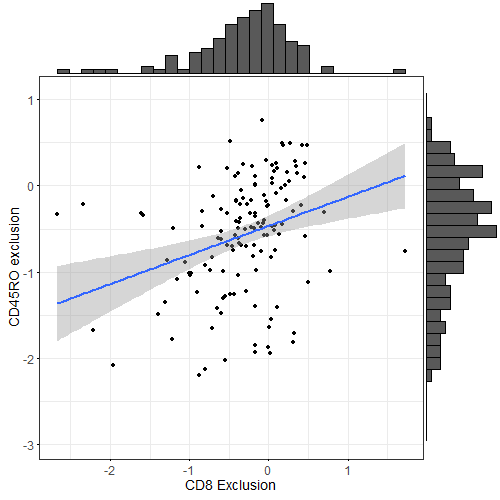
\includegraphics[width=0.5\textwidth]{Chapter2/Figs/Raster/Figurenew_ratio_scatter.png}
    \caption{Immune exclusion ratio of CD8 and CD45RO T-cells. Ratios are log-transformed like the counts. Histograms of exclusion are shown on the graph, both distributions are log-normal.}
    \label{fig:ratio}
\end{figure}



\subsection{Functional form of infiltrates in building a survival model}
When modelling survival using Cox regression, one must assess that the assumptions of the Cox model are met and decide upon the functional form of the predictor\ref{eq:cox}. I utilized Martingale residuals (Figure \ref{fig:martingale} to confirm that the base 10 transformation previously applied successfully addressed the non-linearity of the data. In order to find the best functional form for each predictor I modelled the univariate relationship between the predictor and survival using Cox regression and plotting the residuals of the model fit against the expected form. The relationship between each of the immune variables and survival was found to be approximately log-linear. 

\begin{figure}
    \centering
    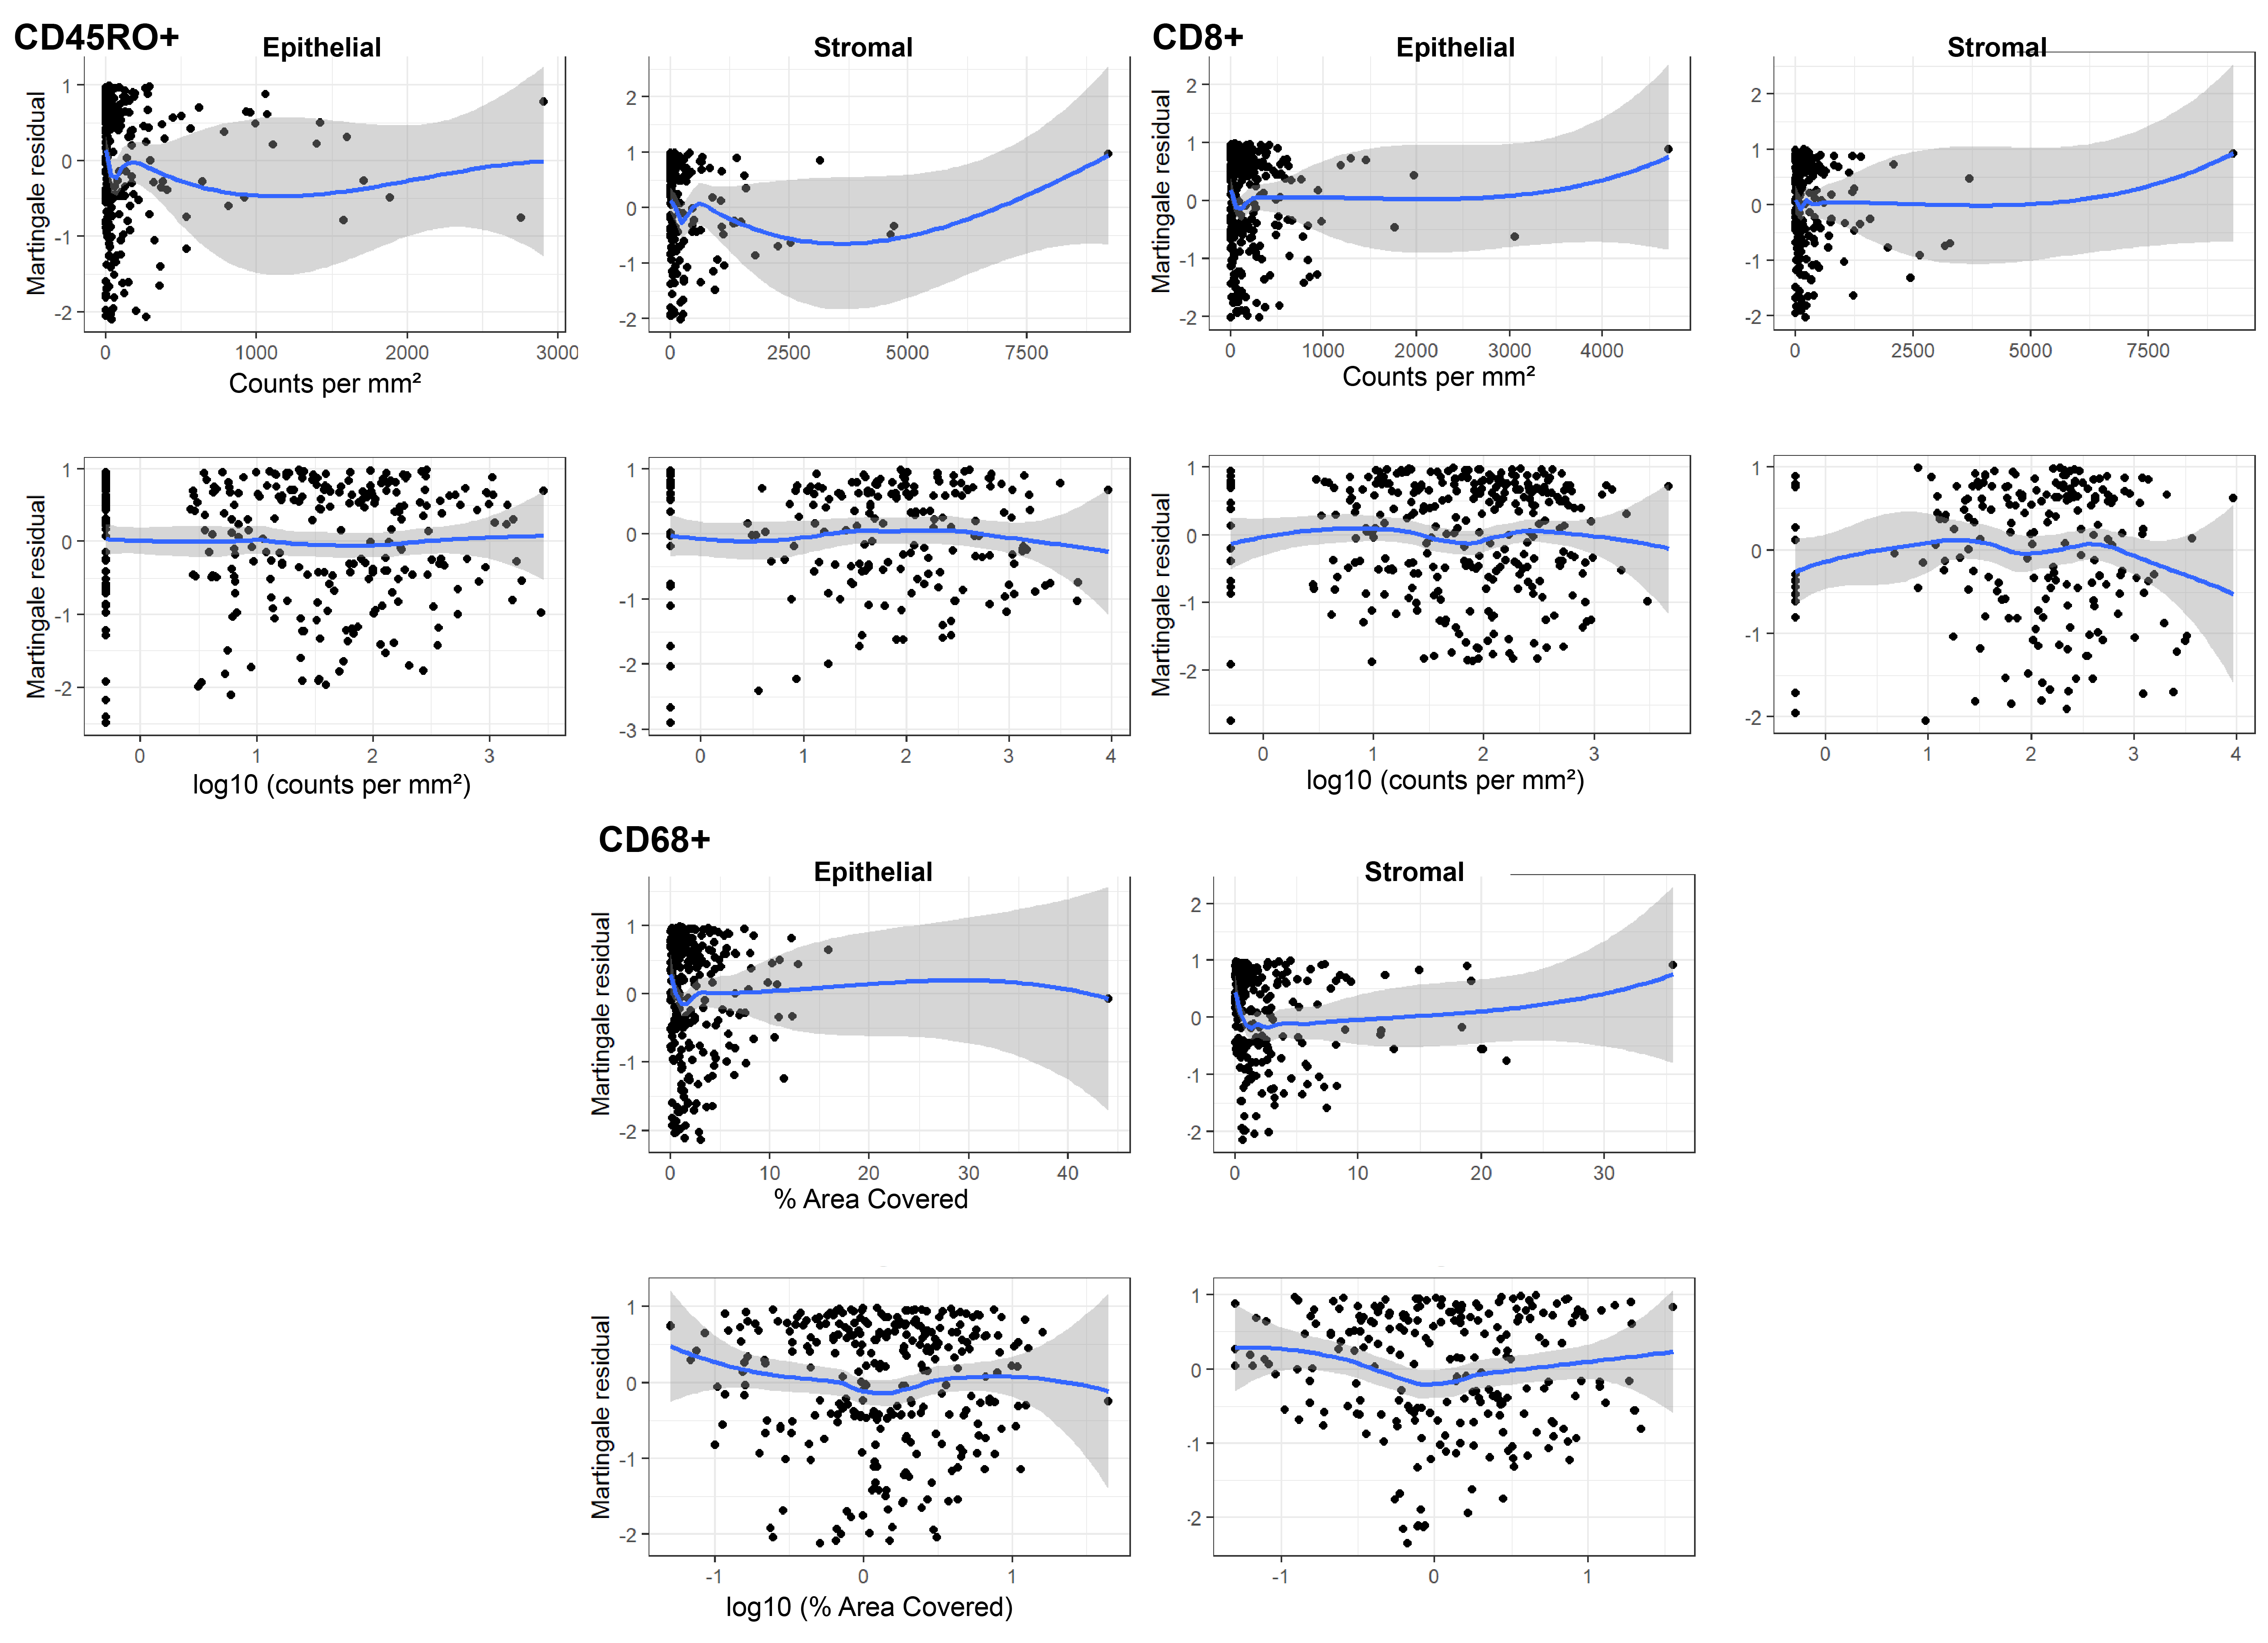
\includegraphics{Chapter2/Figs/Raster/martingale_plots.png}
    \caption{Martingale residuals of each infiltrate assesses the linearity of the variables. The log10 transformation is seen to improve linearity in all cases.}
    \label{fig:martingale}
\end{figure}

The only clinical variables accompanying the cohort were age at diagnosis, stage and menopause status. Age at diagnosis is the only continuous variable of these and the relationship between age and survival was found to be approximately linear (Figure \ref{fig:modelfit}, Table \ref{tab:model_fit}). 

\begin{table}[]
    \centering
    \begin{tabular}{cccc} \hline
        	&	Linear 	&	Cubic splines	&	Log(base 10)	\\
	&	p-value	&	p-value	&	p-value	\\ \hline
Age at diagnosis	&	0.18	&	0.36	&	0.24	\\
CD8$^+$ epithelium	&	0.43	&	0.36	&	0.25	\\
CD8$^+$ stroma	&	0.4	&	0.17	&	0.64	\\
CD68$^+$ epithelium	&	0.44	&	0.57	&	0.63	\\
CD68$^+$ stroma	&	0.09	&	0.06	&	0.009	\\
CD45RO$^+$ epithelium	&	0.3	&	0.09	&	0.07	\\
CD45RO$^+$ stroma	&	0.07	&	0.016	&	0.002	\\
\hline

    \end{tabular}
    \caption[P-values for the association of each functional form of the variable with survival]{P-values for the association of each functional form of the variable with survival using univariable Cox regression analyses. Lowest p-values demonstrate most likely functional form and show that each relationship is approximately log linear}
    \label{tab:model_fit}
\end{table}

\begin{figure}
    \centering
    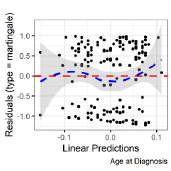
\includegraphics[width=\textwidth]{Chapter2/Figs/Raster/Artboard 39.png}
    \caption[Residuals of model fit]{Residuals of model fit plotted against predicted value for age at diagnosis, the relationship was found to be approximately linear.}
    \label{fig:model_age}
\end{figure}



\subsection[Prognostic value of individual infiltrates]{Stromal CD68$^+$ and CD45RO$^+$ infiltrate are the strongest individual prognostic markers}

Initially I investigated whether survival models of the individual infiltrates in stroma and tumour accurately fit the data. Univariable analysis showed improved survival with increasing stromal density of CD45RO$^+$ (HR 0.76 95\% CI 0.65–0.90, p=0.001) and CD68$^+$(HR 0.53 95\% CI 0.34–0.81, p=0.003) (Table \ref{tab:coxsurv}). Modelling each immune variable with stage showed improved predictive value for epithelial CD8$^+$ density (HR=0.83, p-value=0.027) as well as stromal CD68$^+$ and CD45RO$^+$ density and epithelial CD45RO$^+$ density (Table  \ref{tab:coxsurv}). Kaplan-Meier curves require an arbitary cutpoint for continuous data that impacts reported significance, as such I used these for illustrative purposes only. Figure \ref{fig:kmcd68845}) shows illustrative Kaplan-Meier survival curves for high and low stromal and epithelial CD68$^+$, CD45RO$^+$ and CD8$^+$ densities.\\



\subsection{Averaging immune infiltrate over a core}

In clinical reporting, quantifying immune populations in exclusively tumour epithelium is technically challenging and time consuming. I was therefore interested in testing the value of using the average density of each marker averaged across both tumour and stromal regions from each core (Table \ref{tab:coxsurv}).  Averaging the tissue density of CD8$^+$ increased the strength of the associated hazard ratio and significance of the model (HR=0.79, p-value=0.010) indicating increased prognostic value for CD8$^+$ infiltrate over quantitation of individual epithelial and stromal infiltrates. The significance did not increase for CD45RO$^+$ and CD68$^+$ infiltrates.  Figure \ref{fig:KM_infiltrates} shows illustrative Kaplan-Meier survival curves for high and low CD68$^+$, CD45RO$^+$ and CD8$^+$ densities over combined epithelium and stroma compartments.\\


\begin{landscape}
\begin{table}[]
    \centering
    \begin{tabular}{llllllll}
    
		& & &&		Univariable && \multicolumn{2}{c}{	Multivariable* 
(adjusted for stage)} \\
								
&	Functional Form &	Evaluable cases&	Tissue compartment&	HR &	p-value	& HR &	p-value	\\ \hline
CD8$^+$&	log10 &	301	&Epithelium&	0.89&	0.15&	0.83&	0.027\\	
&	log10&	202&	Stroma&	0.97&	0.74&	0.93&	0.40\\	
&	log10&	315&	Average&	0.79&	0.010&	0.72&	0.0006\\	
CD45RO+&	log10&	290&	Epithelium&	0.86&	0.033&	0.85&	0.022\\	
	&log10&	196&	Stroma&	0.76&	0.001&	0.76&	0.0007\\	
	&log10&	306&	Average&	0.82&	0.006&	0.80&	0.003\\	
CD68+&	linear&	293&	Epithelium&	0.99&	0.67&	0.99&	0.43\\	
&	log10&	226	&Stroma	&0.53&	0.003&	0.44&	0.0003	\\
&	log10&	308	&Average&	0.67&	0.042&	0.62&	0.017\\	
Stage1 & - &	312&	Localised&	1&	0&	1&	0	\\
	& & &		Regional&	1.47&	0.26&	1.15&	0.25\\	
	&	&&	Distant	&3.96&	<<0.001&	5.58&	<<0.001	\\
	&	&&	Unstaged&	3.35&	<0.001&	3.34&	<<0.001	\\ \hline

\end{tabular}
    \caption[Individual immune infiltrates Cox regression]{Cox proportional hazards survival analysis for individual infiltrates.}
    \label{tab:coxsurv}
\end{table}
\end{landscape}

\begin{figure}
    \centering
    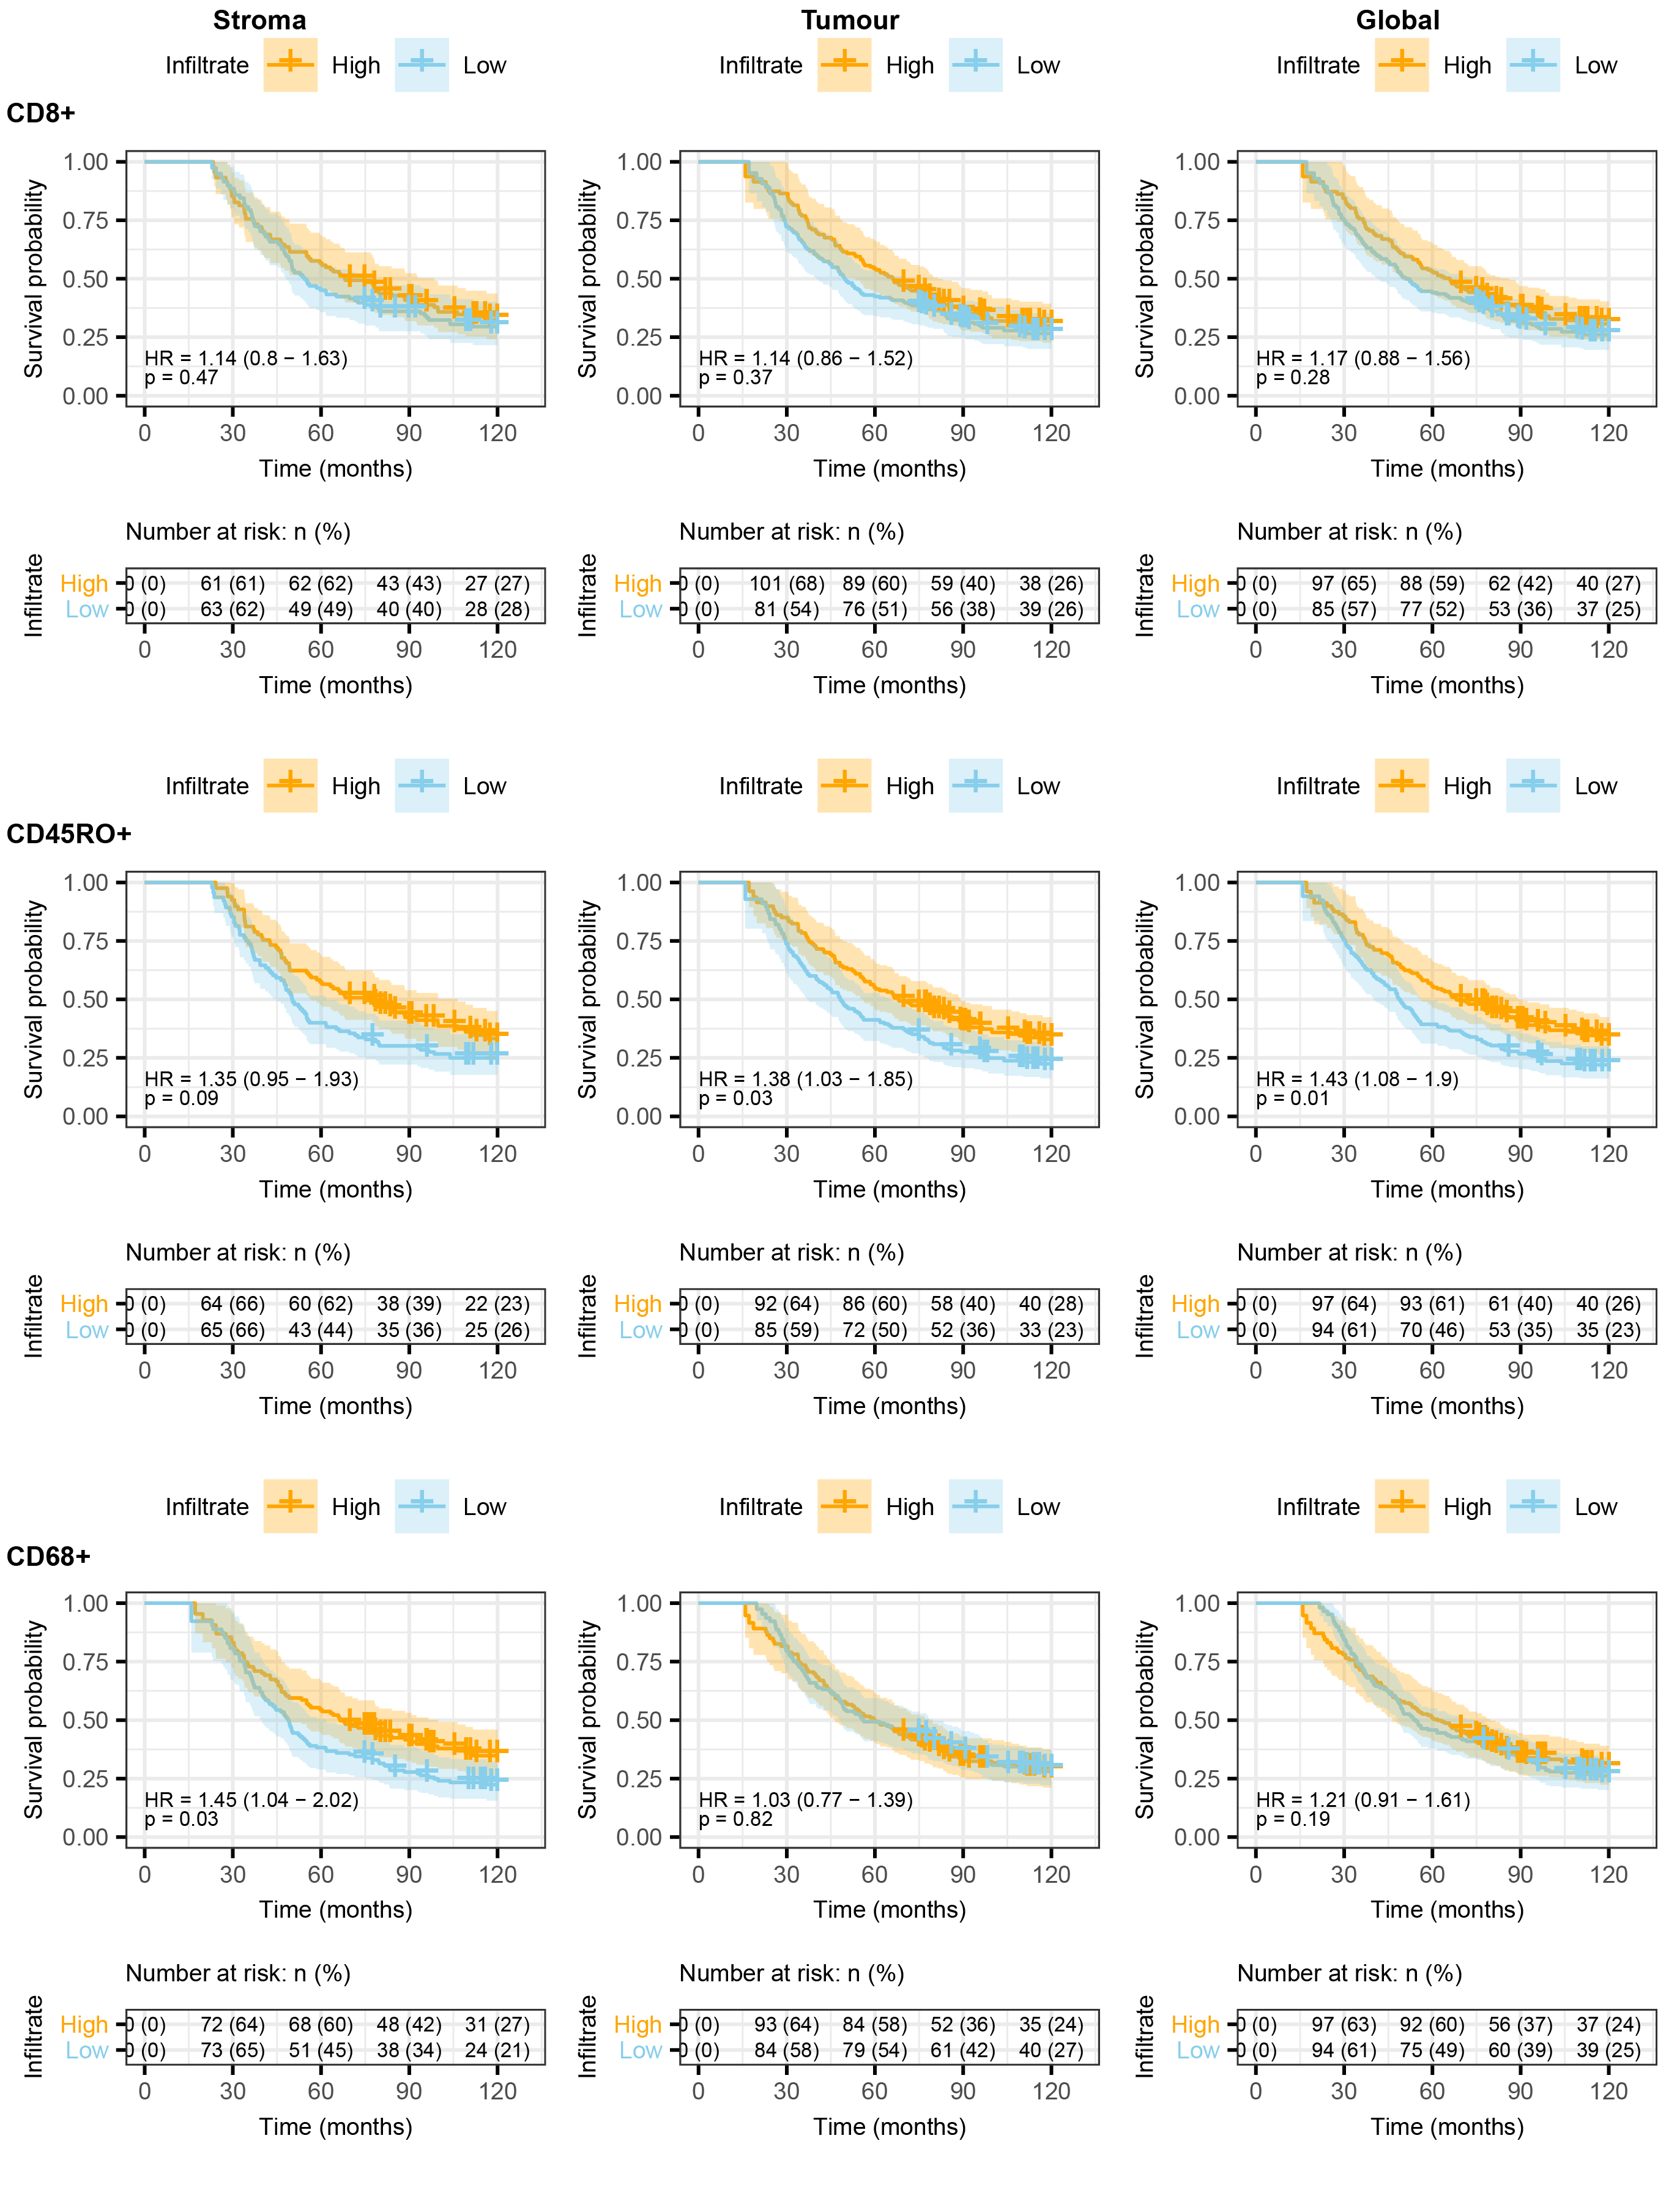
\includegraphics{Chapter2/Figs/Raster/KM_allinf.png}
    \caption[KM Survival curves for individual infiltrates]{Kaplan–Meier survival curves using cut point of median density of stromal CD68$^+$ macrophages and CD45RO$^+$ memory T cells using left truncation and right censoring. Median entry to the study for all patients after diagnosis was 26.4 months. Median follow up time from diagnosis to exit or death was 105.1 months.}
    \label{fig:KM_infiltrates}
\end{figure}

\subsection{Epithelial core subset survival analysis}

Alongside assessing cores with both tumour and stroma and consequently assessing the survival impact of immune cells in a stromally infiltrated environment, I wanted to test these associations in purely epithelial cores. I asked whether CD45RO$^+$ and CD8$^+$ epithelial infiltrate were still significant predictors in predominantly epithelial cores. In the separate subset of cores with <1\% stroma, epithelial CD8$^+$ malignant epithelial infiltrate remained an independent prognostic factor but epithelial CD45RO$^+$ density was not significant (n=110,p=0.78)(Table \ref{tab:surv_cd8_epi}).

\begin{table}[]
    \centering
    \begin{tabular}{cccccc}\hline 	&		&	\multicolumn{2}{l}{Univariable}			&	\multicolumn{2}{l}{Multivariable*}			\\
 	&	Cases	&	HR	&	p-value	&	HR	&	p-value	\\ \hline
CD8+	&	111	&	0.84	&	0.27	&	0.7	&	0.047	\\
CD45RO+	&	110	&	0.98	&	0.89	&	0.96	&	0.78	\\
CD68+	&	80	&	1.21	&	0.47	&	1.27	&	0.39	\\
\hline
    \end{tabular}
    \caption[Epithelial core immune infiltrate and survival]{Cox proportional hazard regression for cores with malignant epithelial tissue only. Multivariable analysis includes stage.}
    \label{tab:surv_cd8_epi}
\end{table}


\subsection{Combined model}

Given that individually, all infiltrates were prognostic in at least one compartment, the next step was to model the survival of patients based on all infiltrates together to account for the different effects of differing infiltrates. I carried out multivariable Cox regression analysis including all infiltrates and stage on patients with complete data for all infiltrates (n=152) (Table \ref{tab:cox_combined}).  In this model only stage and CD68$^+$ stromal infiltrate were significant predictors of survival.

I then refined the model by removing the least significant elements (defined as those with p>0.1) (Table \ref{tab:cox_combined}, n=152). Interestingly, I found that the p-values for CD68$^+$ and CD45RO$^+$ stromal infiltrates in the refined model become less significant and the hazard ratios are attenuated in comparison to both the univariable regression and the full model. This is likely due to the inability of Cox regression to distinguish with confidence whether stromal CD45RO$^+$ or CD68$^+$ density is the most significant predictor when there is a strong correlation between all the immune variables.
\begin{table}[]
    \centering
    \begin{tabular}{llcccc} \hline
&&	Multivariable & (all combined) &	Refined model &\\ 
	&&	HR&	p-value&	HR&	p-value\\ \hline
CD8+&	Epithelium&	0.96&	0.81&	-	&-\\
	&Stroma&	1.07	0.63	&-&	-\\
CD45RO+&	Epithelium&	1.12&	0.37	&-&	-\\
	&Stroma	&0.83	&0.09	&0.68&	0.11\\
CD68+&	Epithelium&	1.16&	0.63	&-&	-\\
	&Stroma	&0.53&	0.038&	0.88	&0.17\\
Stage &&&&&\\
&Localised&	1&	0&	1&	0\\
&	Regional&	2.00&	0.16&	2.03&	0.14\\
&	Distant&	4.82&	<<0.001&	4.70&	0.0001\\
&	Unstaged	&8.15&	<<0.001&	8.25&	0.0001\\ \hline

    \end{tabular}
    \caption[Cox regression HR and p-values for combined and reduced survival models.]{Cox proportional hazard regression HR for combined and reduced models. The Refined model is reduced down from all infiltrates to attempt to improve the model. Stage is included in both models.}
    \label{tab:cox_combined}
\end{table}

\subsection{Is the ratio of stromal T-cell infiltrate to intra-epithelial T-cell infiltrate prognostic?}

Immune exclusion and the location of immune infiltrate in either the intra-epithelial or stromal regions is a spatial micro-environmental property that can easily be derived from images. The ratio of tumour to stromal infiltrate may indirectly measure properties of the ECM that allow for infiltration into the tumour core or measure the extent of the interaction of the immune cells with epithelial cells. As shown previously, stromal and intra-epithelial immune cell densities are correlated. I investigated whether the ratio of stromal infiltrate density to intra-epithelial immune infiltrate density was a significant predictor of risk in HGSOC using the Cox proportional hazards model.

% latex table generated in R 3.3.2 by xtable 1.8-2 package
% Thu Oct 19 15:01:03 2017
\begin{table}[ht]
\centering
\begin{tabular}{llllll} \hline
 	&		&	\multicolumn{2}{l}{Univariable}			&	\multicolumn{2}{l}{Multivariable}			\\
 	    &	n	&	HR	&	p-value	    &	HR	&	p-value	\\ \hline
CD8	    &	188	&	0.94	&	0.65	&	0.95	&	0.69	\\
CD45RO	&	180	&	1.13	&	0.36	&	1.28	&	0.20	\\
CD68	&	211	&	1.53	&	0.09	&	1.54	&	0.018	\\

   \hline
\multicolumn{5}{l}{}\\
\end{tabular}
\caption[Cox regression for ratio of Tumour to Stroma infiltrate]{Single predictor Cox proportional hazard tests with ratios of stromal to tumour infiltrate as predictors.} 
\label{tab:s:t}
\end{table}
There is no significant effect on survival of stroma:tumour ratio for the T-cell subsets. The ratio of tumour:stroma macrophages however has an impact upon survival, with a higher epithelial:stromal infiltration ratio having a negative impact upon survival (Table \ref{tab:s:t}, $p=0.018, \mathrm{HR}=1.54$).

\subsection{Principal components and the combined immunospace}
 Part of the problem that I encountered in analysing the effect of multiple immune populations upon survival is that the multiple immune infiltrates are correlated (see Figure \ref{fig:ch2_correlation}) and may have additive or suppressive effects.  In order to assess the multi-dimensional nature of the immune response in more detail I proposed that as the three types of immune infiltrate vary continuously across epithelium and stroma these variables can be regarded as six dimensions of an ‘immunospace’ (three infiltrates, 2 localizations).  Given the strong correlations between infiltrates (Figure \ref{fig:ch2_correlation}), we can safely say these immune variables are not independent. I used principal component analysis (PCA) to determine the independent patterns across these dimensions, using the 152 patients for whom complete data were available.
 
 PCA transformed the six correlated infiltrate variables into six independent axes with the first component containing the largest proportion of variance (60\%) in the data set\ref{tab:PC}. Patients are plotted by their PC1 and PC2 values in Figure \ref{fig:PC_plot}. In principal component 1 (PC1), the weightings of all immune infiltrates are positive and similar in magnitude (Table \ref{tab:PC}). This indicates that as one infiltrate increases so do all the others and represents the degree of coordinated immune response. The remaining principal components characterize additional patterns across immune infiltrates independent of PC1. The additive contribution of PC2 characterises negative correlation between CD8$^+$ infiltrates and CD68$^+$ macrophages and CD45RO$^+$ memory cells. PC3 characterizes additional variation where epithelial and stromal infiltrates are negatively correlated, the most positive values of PC3 correspond to high infiltration in tumour epithelium compared to stroma and the most negative values of PC3 correspond to the opposite, the aforementioned immune exclusion. 
 
\begin{table}[]
    \centering
    \begin{tabular}{lllllll}\hline
&PC1& PC2&PC3&PC4&PC5&PC6\\
&(60\%)&(13\%)&(9\%)&(8\%)&(5.5\%)&(4.5\%)\\
\hline
CD8$^+$ tumour density& 0.38&-0.56&0.58&-0.1&0.4&-0.21\\
CD8$^+$ stromal density&0.38&-0.59&-0.47&0.27&-0.21&0.43\\
CD68$^+$ tumour density&0.41&0.47&0.37&0.11&0.09&0.67\\
CD68$^+$ stromal density&0.42&0.3&-0.29&0.56&0.36&-0.45\\
CD45RO$^+$ tumour density&0.45&0.11&0.21&-0.07&-0.78&-0.36\\
CD45RO$^+$ stromal density&0.41&0.15&-0.42&-0.77&0.22&-0.03\\
\hline
    \end{tabular}
    \caption[Composition of the principal components across all infiltrates]{Contributions of normalized infiltrates to all principal components. Figures in brackets indicate proportion of total variance}
    \label{tab:PC}
\end{table}

\begin{figure}
    \centering
    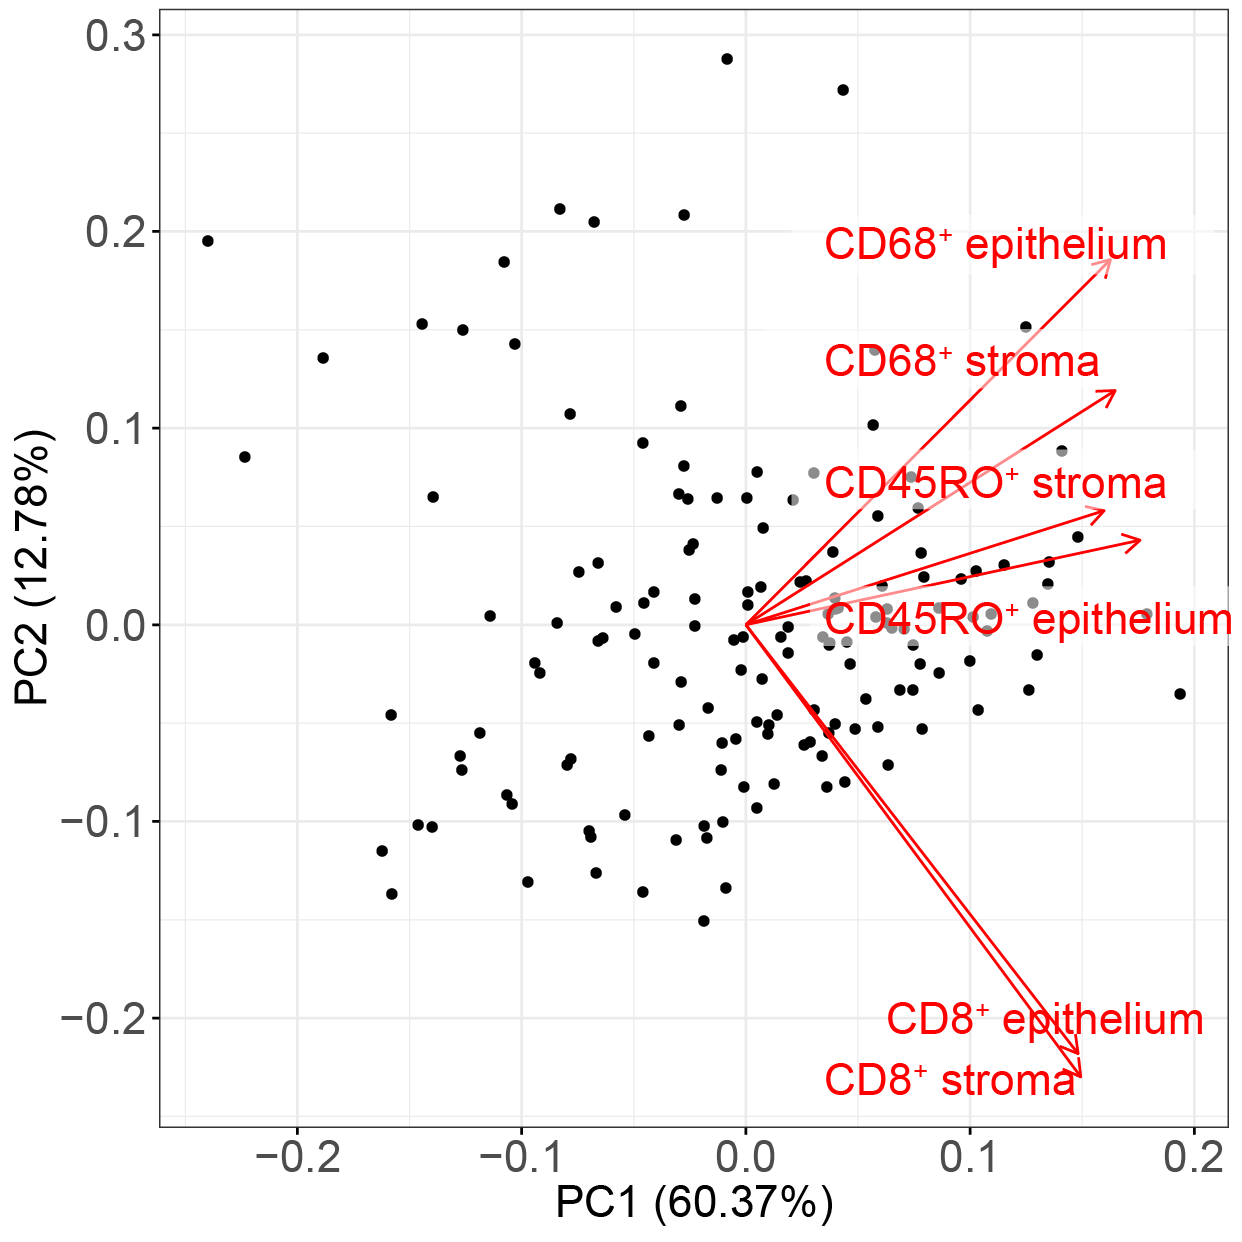
\includegraphics{Chapter2/Figs/Raster/PCA_xy.png}
    \caption{Patients plotted on axes giving their values of Principal Component 1 and 2.}
    \label{fig:PC_plot}
\end{figure}
 
Having calculated the principal components from the data, it is possible to extract the patients who lie at the most extreme ends of these axes of variation. Figure \ref{fig:PC_examples} shows representative images with the largest magnitudes of PC1, PC2 and PC3 to visually illustrate the patterns described above. This figure demonstrates especially clearly the coordinated immune infiltration and the immune exclusion that are described by PC1 and PC3. 

The variance in the remaining principal components (4-6) is smaller and less informative. Variance in PC4 is predominantly from CD45RO$^+$ stromal density, PC5 is from CD45RO$^+$ epithelial density and PC6 is from CD68$^+$ epithelial density. 


In order to evaluate the prognostic impact of these patterns of infiltration, I used Cox proportional hazard regression to assess whether these principal components were predictive of survival. Cox regression survival models were also calculated on all combinations of principal components and stage. Only PC1 was an independent predictor of survival in this cohort and was associated with improved survival (Univariate: HR=$0.89$, $p=0.024$, PC1+Stage: HR: $0.88$, $p=0.019$) (Table \ref{tab:pc_surv}) reflecting the good prognosis of a strong coordinated immune response. The association of this principal component with survival is also illustrated graphically using Kaplan Meier curves in Fig. \ref{fig:km_PC}.

\begin{landscape}
\begin{figure}[width=0.8\textwidth, keepaspectratio]
    \centering
    \includegraphics[width=\textwidth]{Chapter2/Figs/Raster/PC_montfort.png}
    \caption[Examples of tissue sections with largest values of principal components.]{Images of the sections of patients with the highest values of principal components 1, 2 and 3. The values of the immune infiltrates of these images are shown on the boxplots of the distribution across all samples.}
    \label{fig:PC_examples}
\end{figure}
\end{landscape}

\begin{figure}
    \centering
    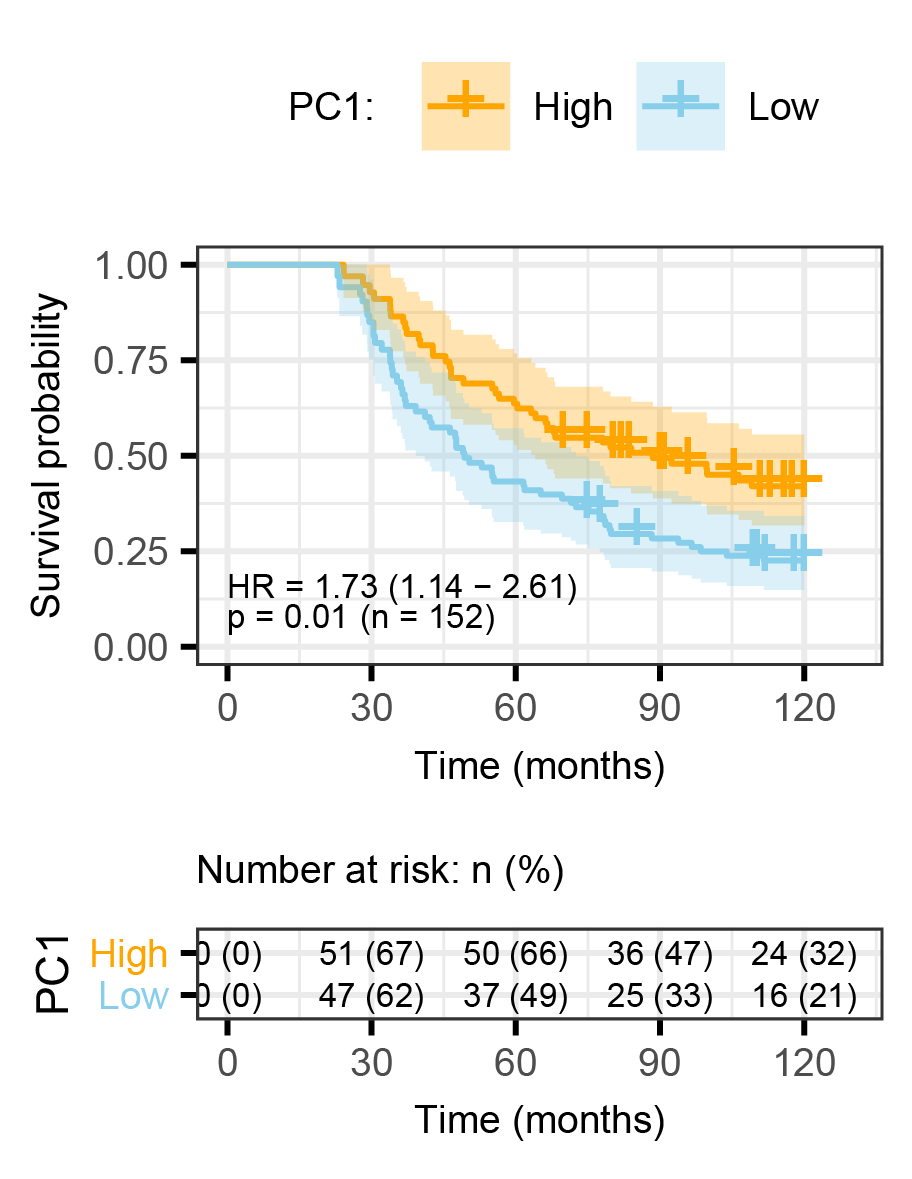
\includegraphics{Chapter2/Figs/Raster/Montfort-2018_Fig7A-PC1.png}
    \caption[Kaplan Meier Curves for Principal Component 1]{Kaplan Meier illustrative survival curve. Principal component 1 are split at the median. The survival of high and low values of Principal component 1 are plotted against time. }
    \label{fig:km_PC}
\end{figure}

\begin{table}[]
    \centering
    \begin{tabular}{lllll} \hline
         	&	\multicolumn{2}{l}{Univariable}			&	\multicolumn{2}{l}{Multivariable}			\\
 	&	HR	&	p-value	&	HR	&	p-value	\\ \hline
PC1	&	0.89	&	0.024	&	0.88	&	0.016	\\
PC2	&	0.94	&	0.61	&	0.92	&	0.52	\\
PC3	&	1.2	&	0.2	&	1.23	&	0.18	\\
PC4	&	1.14	&	0.43	&	1.07	&	0.69	\\
PC5	&	0.82	&	0.31	&	0.74	&	0.11	\\
PC6	&	1.25	&	0.23	&	1.22	&	0.33	\\ \hline

    \end{tabular}
    \caption[Cox proportional hazard regression for principal components]{Cox proportional hazard regression for principal components as predictors. Multivariable analysis includes stage.}
    \label{tab:pc_surv}
\end{table}

\subsection{Comparing Survival Models}
 The Akaike Information Criterion (AIC) was used to compare the performance of these survival models and includes a penalty on the number of terms to reduce over-fitting (Supplementary Fig. 8). The model combining stage, PC1 and PC5 had the best performance for predicting overall survival. The improvement with the addition of PC5 shows that the addition of this principal component has a suppressor effect in the model, increasing the significance of other variables when included. This demonstrates that survival is predominantly determined by the coordinated immune response and further variation in survival from this trend can be encoded by the quantity of epithelial CD45RO$^+$ infiltrate. Interestingly, the models that contained stage and either stromal CD45RO$^+$ or CD68$^+$ infiltrate contained a similar amount of information about patient survival as the one that contained stage and principal components 1 and 5. In our cohort, the density of CD68$^+$ and CD45RO$^+$ stromal infiltrates are therefore the best single infiltrates for survival modelling. 
 
 \begin{figure}
     \centering
     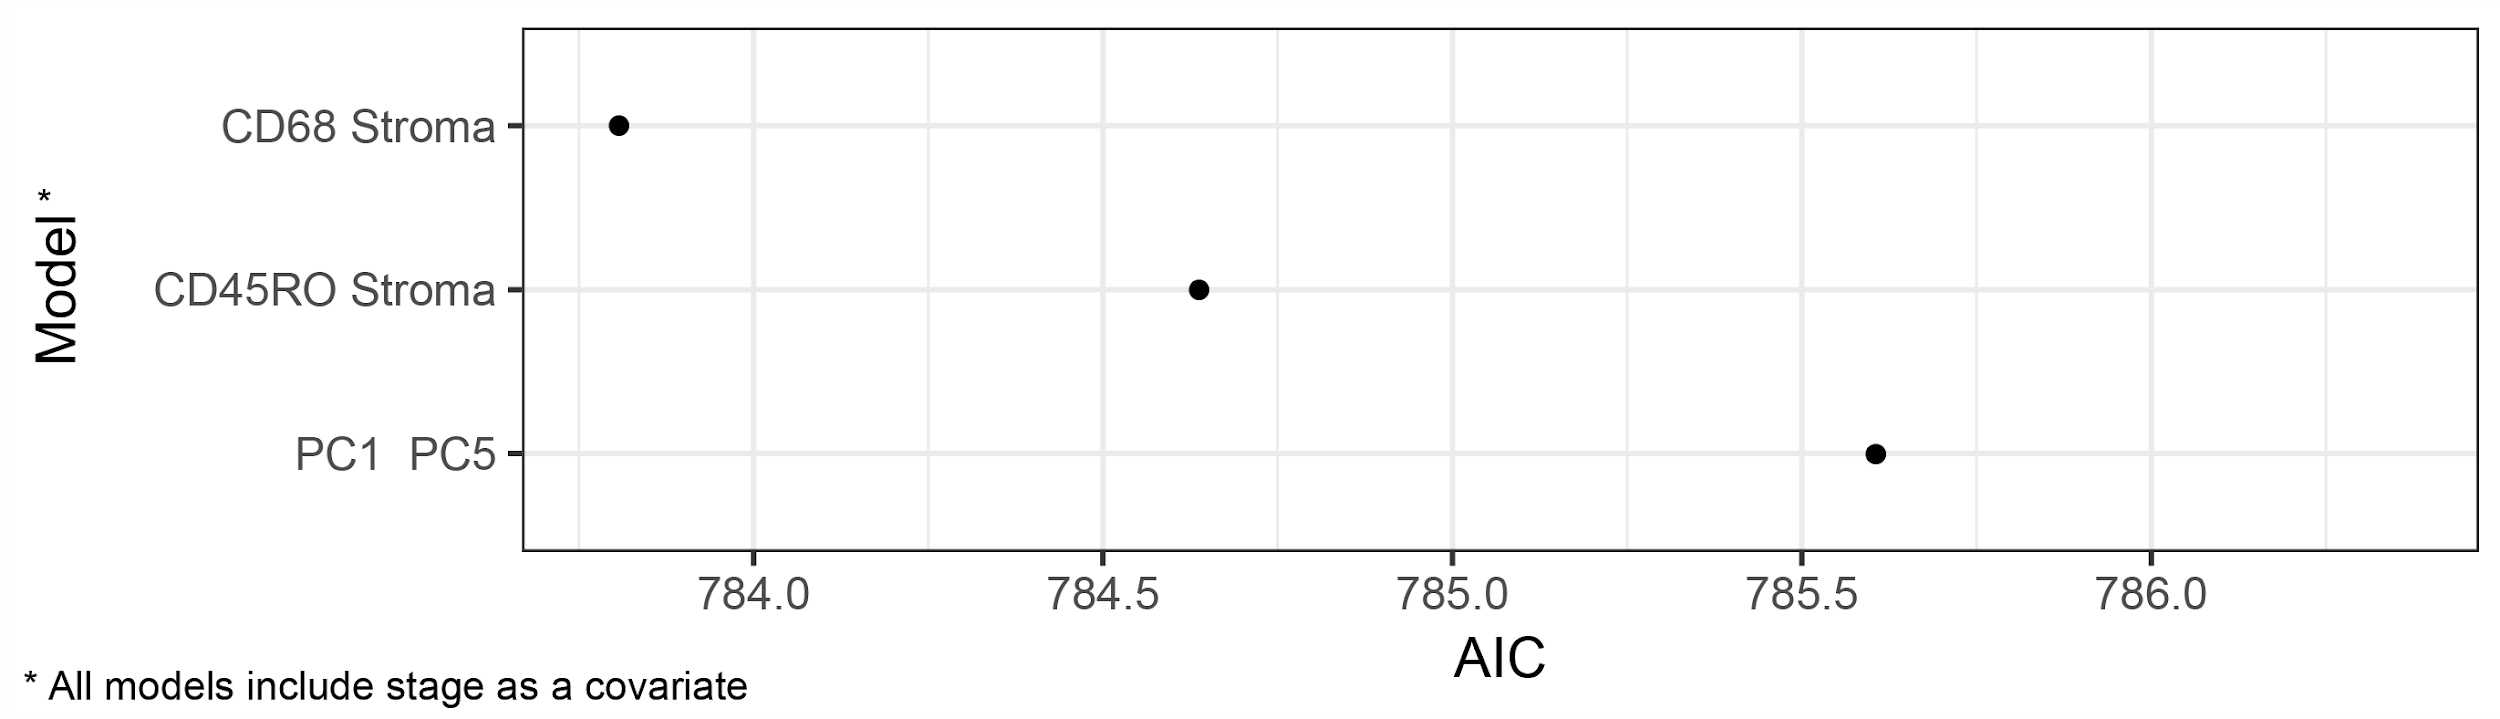
\includegraphics[width=\textwidth]{AIC}
     \caption{AIC for most significant models (AIC > 2)}
     \label{fig:AIC}
 \end{figure}


\subsection{Are genetic defects associated with HGSOC driving individual infiltrates or the coordinated immune response in tumours?}

\subsubsection*{Infiltrate density is not significantly associated with \textit{BRCA} status}
To investigate the interactions between the TME and the genome, can ask whether a germline mutation in either of the \textit{BRCA1/2} genes results in changes in the TME and specifically the immune infiltrate. I investigated whether tumour, stroma or full core measures of CD8$^+$, CD45RO$^+$or CD68$^+$densities were related to \textit{BRCA1/2} mutations using the Kruskal-Wallis rank sum test. I compared the infiltrate density distributions between patients with no mutation, a mutation in \textit{BRCA1} and a mutation in \textit{BRCA2}. I found that the distributions of CD8$^+$, CD45RO$^+$and CD68$^+$infiltrates and the principal components were not significantly associated with \textit{BRCA} mutation status (Figure \ref{fig:genomic}). This was unexpected as previous results have found increases in CD8$^+$infiltrate with a \textit{BRCA1} mutation\cite{Clarke2009}.

\begin{figure}
    \centering
    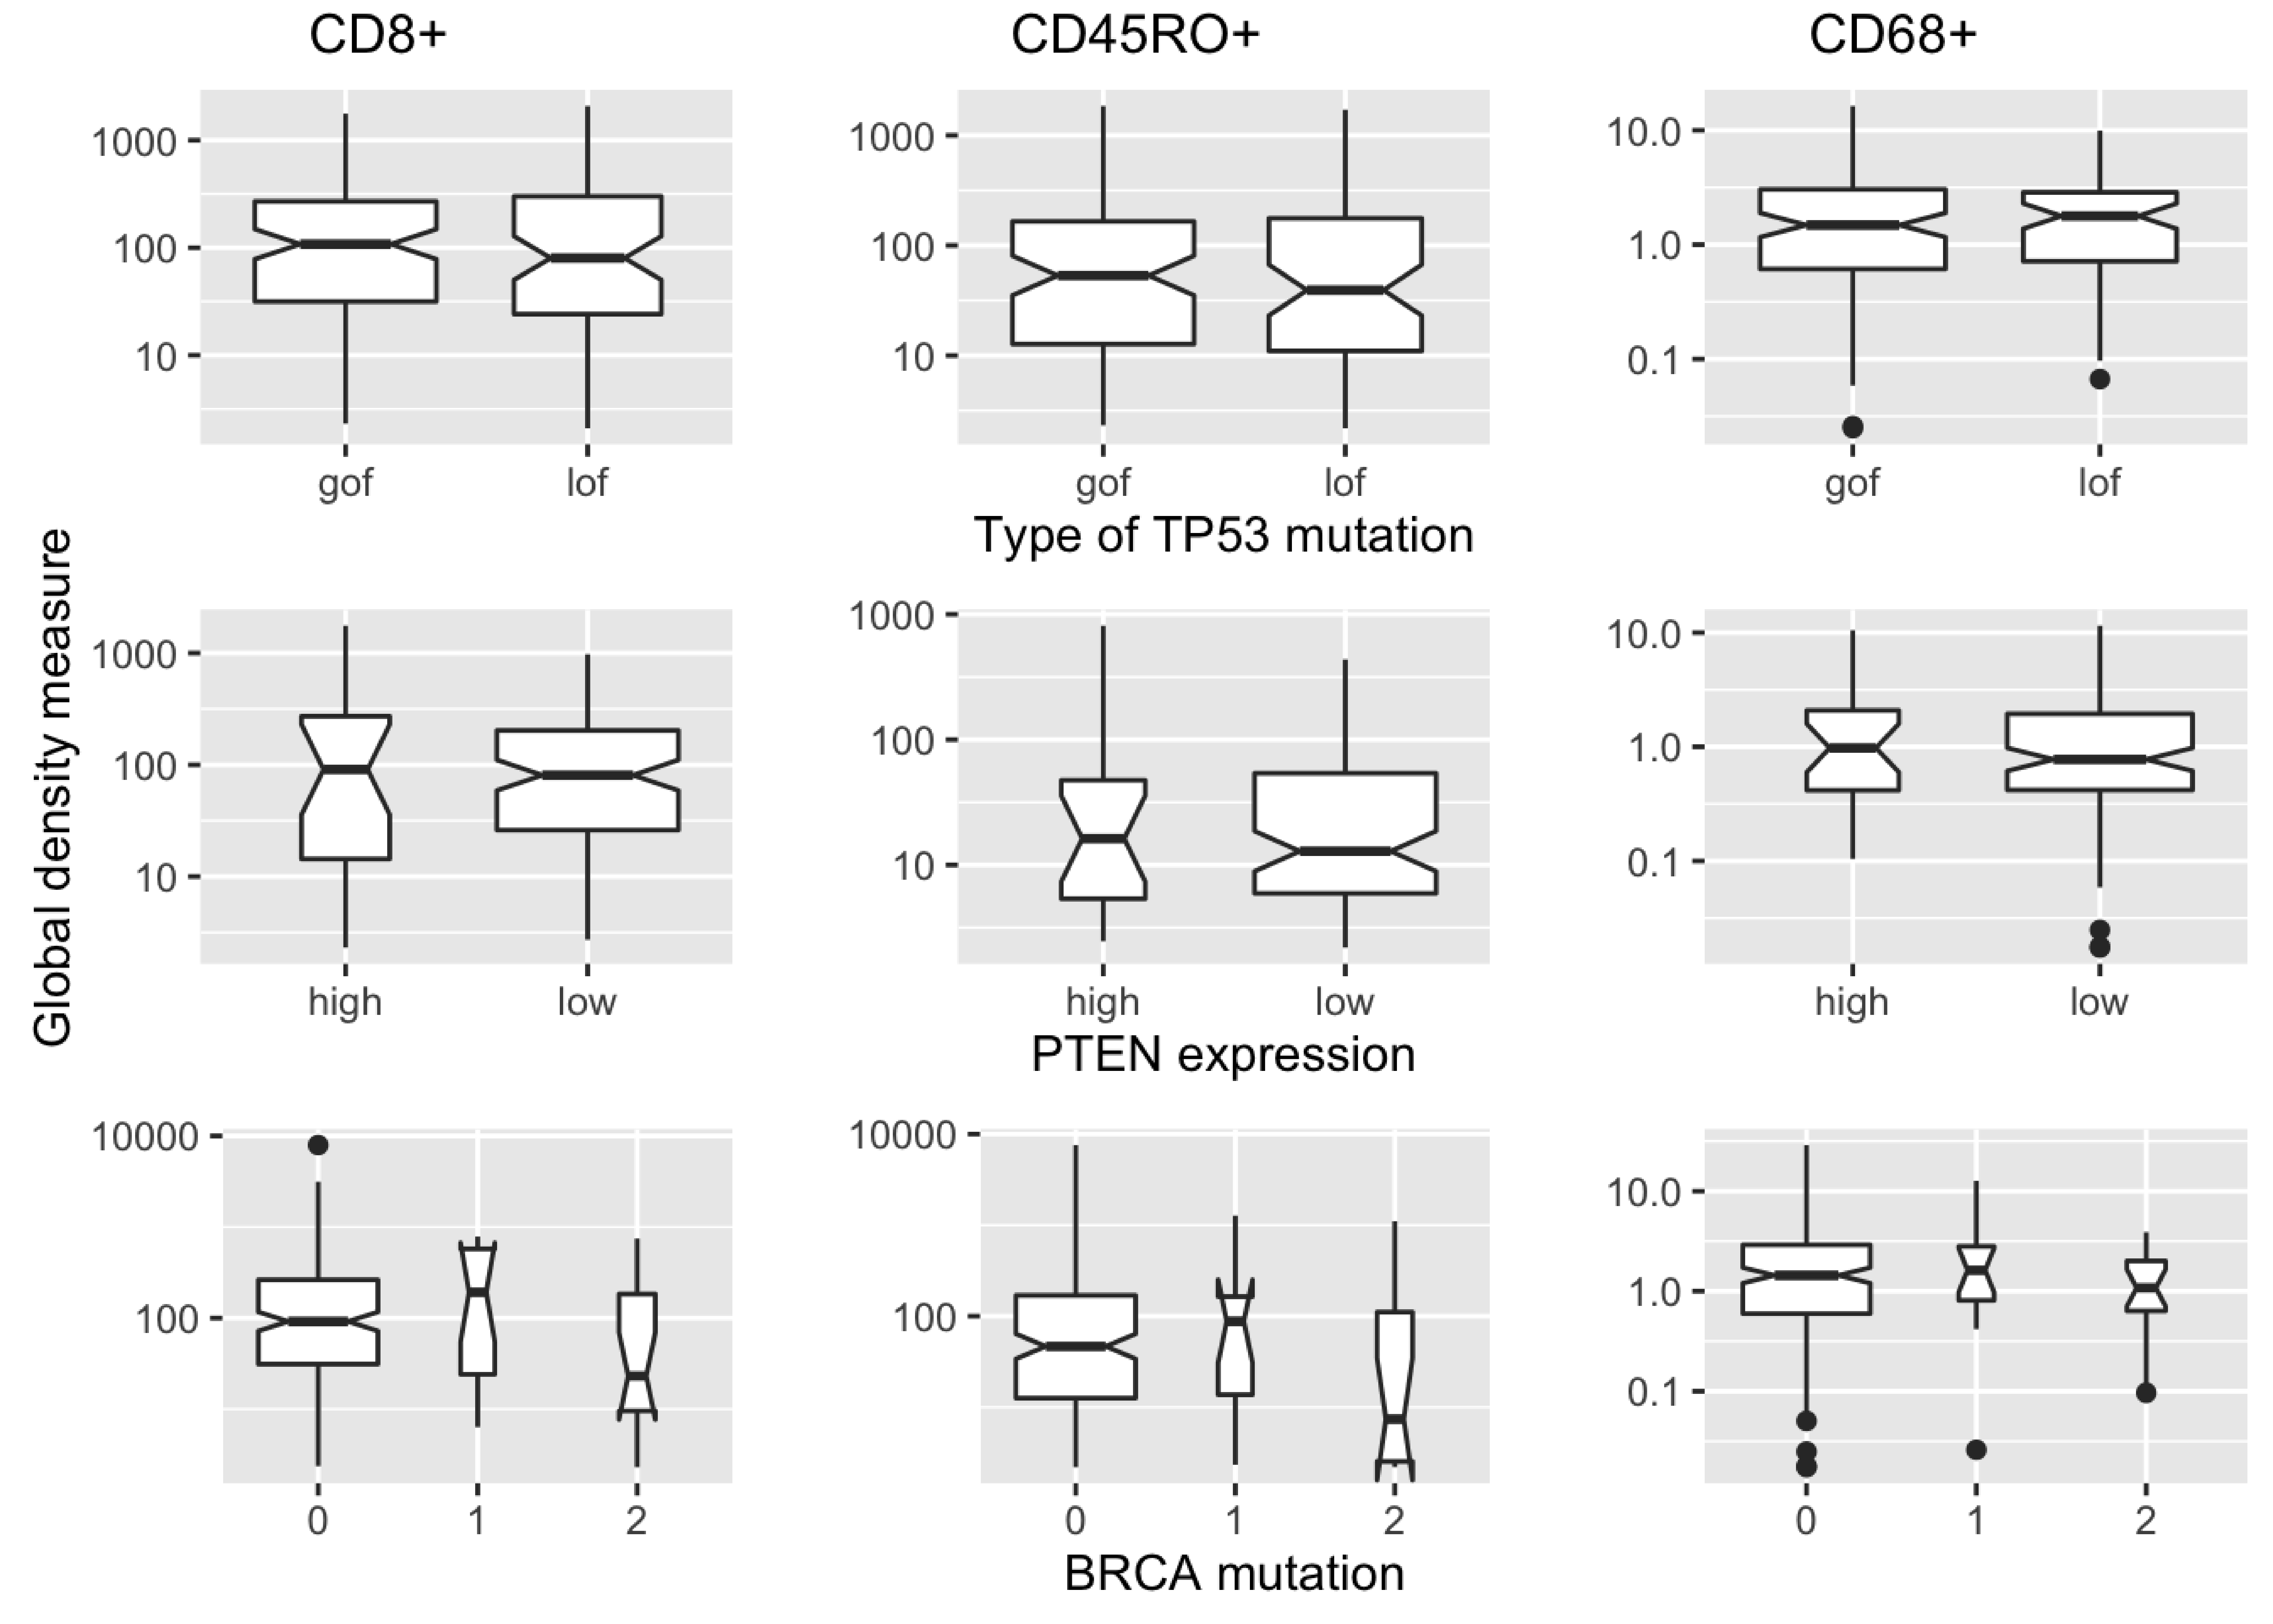
\includegraphics[width=\textwidth]{Chapter2/Figs/Raster/genomic.png}
    \caption{Boxplots of Infiltrate distribution against genomic phenotype.}
    \label{fig:genomic}
\end{figure}

\subsubsection{Infiltrate density is not significantly associated with type of \textit{TP53} mutation.}
Mutant P53 proteins have been linked to multiple micro-environmental changes\cite{Cordani2016}. I investigated whether the type of TP53 mutation produced measurable changes in the TME. Tumour, stroma or full core measures of CD8$^+$, CD45RO$^+$or CD68$^+$densities were compared between gain or loss of function mutations in \textit{TP53}. I used the Kruskal-Wallis rank sum test and found that the distribution of immune infiltrate was not significantly associated with type of \textit{TP53} mutation.

\subsubsection{Infiltrate density is not significantly associated with change in PTEN expression.}
Changes in PTEN expression are cell-intrinsic and levels of PTEN expression are prognostic in HGSOC\cite{RN17, RN15}. Tumour, stroma or full core measures of CD8$^+$, CD45RO$^+$ or CD68$^+$ densities were compared between patients with high or low PTEN expression as measured by both IHC and IF. Using the Kruskal-Wallis rank sum test I found that change in PTEN expression was not significantly associated with any change in the density of immune infiltrate. This particular cell-intrinsic change is not associated with a change in immune infiltration in our cohort.

The presence of germline \texit{BRCA2} mutations was significantly associated with lower CD8$^+$ cell density than patients with a \texit{BRCA1} after multiple testing correction (Figure \ref{fig:genomic}). There was no significant association between the quantity of CD45RO$^+$ or CD68$^+$ infiltrate and the mutational status of either \texit{BRCA1} or \texit{BRCA2} genes (Figure \ref{fig:genomic}) . No significant association was detected between TP53 GOF and LOF mutations or PTEN expression and the densities of CD8$^+$, CD45RO$^+$ and CD68$^+$ cells in epithelium or stroma (Table \ref{tab:}). Similarly, changes in the principal components were not significantly associated with PTEN expression, TP53 GOF or LOF mutation or germline \textit{BRCA1}/\texit{BRCA2} mutation status (Table \ref{tab:genomic}). 




\begin{table}[]
    \centering
    \begin{tabular}{lllll} \hline
     	&		&	\textit{BRCA1/ BRCA2}	&	p53 GOF/LOF	&	PTEN	\\ \hline
CD8+	&	Epithelium	&	0.04	&	0.54	&	0.67	\\
	&	Stroma	&	0.17	&	0.29	&	0.07	\\
	&	Average	&	0.17	&	0.53	&	0.84	\\
CD45RO+	&	Epithelium	&	0.2	&	0.42	&	0.92	\\
	&	Stroma	&	0.46	&	0.84	&	0.82	\\
	&	Average	&	0.1	&	0.36	&	0.87	\\
CD68+	&	Epithelium	&	0.43	&	0.72	&	0.79	\\
	&	Stroma	&	0.78	&	0.85	&	0.65	\\
	&	Average	&	0.68	&	0.66	&	0.41	\\
Principal Component	&	1	&	0.81	&	0.8	&	0.55	\\
	&	2	&	0.1	&	0.26	&	0.17	\\
	&	3	&	0.27	&	0.58	&	0.51	\\
	&	4	&	0.58	&	0.99	&	0.17	\\
	&	5	&	0.76	&	0.88	&	0.79	\\
	&	6	&	0.97	&	0.44	&	0.18	\\
    \hline
    \end{tabular}
    \caption[Significance of Kruskal Wallis tests of infiltrate against genomic subtype]{P-values associated with Kruskal Wallis test for detecting differences in mean ranks of immune infiltrate in patients grouped by mutation in BRCA1, BRCA2 or not-detected, p53 gof or lof and PTEN high or low in HGSOC.}
    \label{tab:genomic}
\end{table}

\subsection{Other ovarian cancer subtypes}

The automated and reproducible nature of this workflow means similar analyses are easily transposed across to the same immune populations assessed in the other subtypes of Ovarian cancer. Due to the smaller numbers of patients with these subtypes, survival analysis was limited to the X population. Figure \ref{fig:morph_area} shows the areas of epithelium and stroma across all OC subtypes.

\begin{figure}
    \centering
    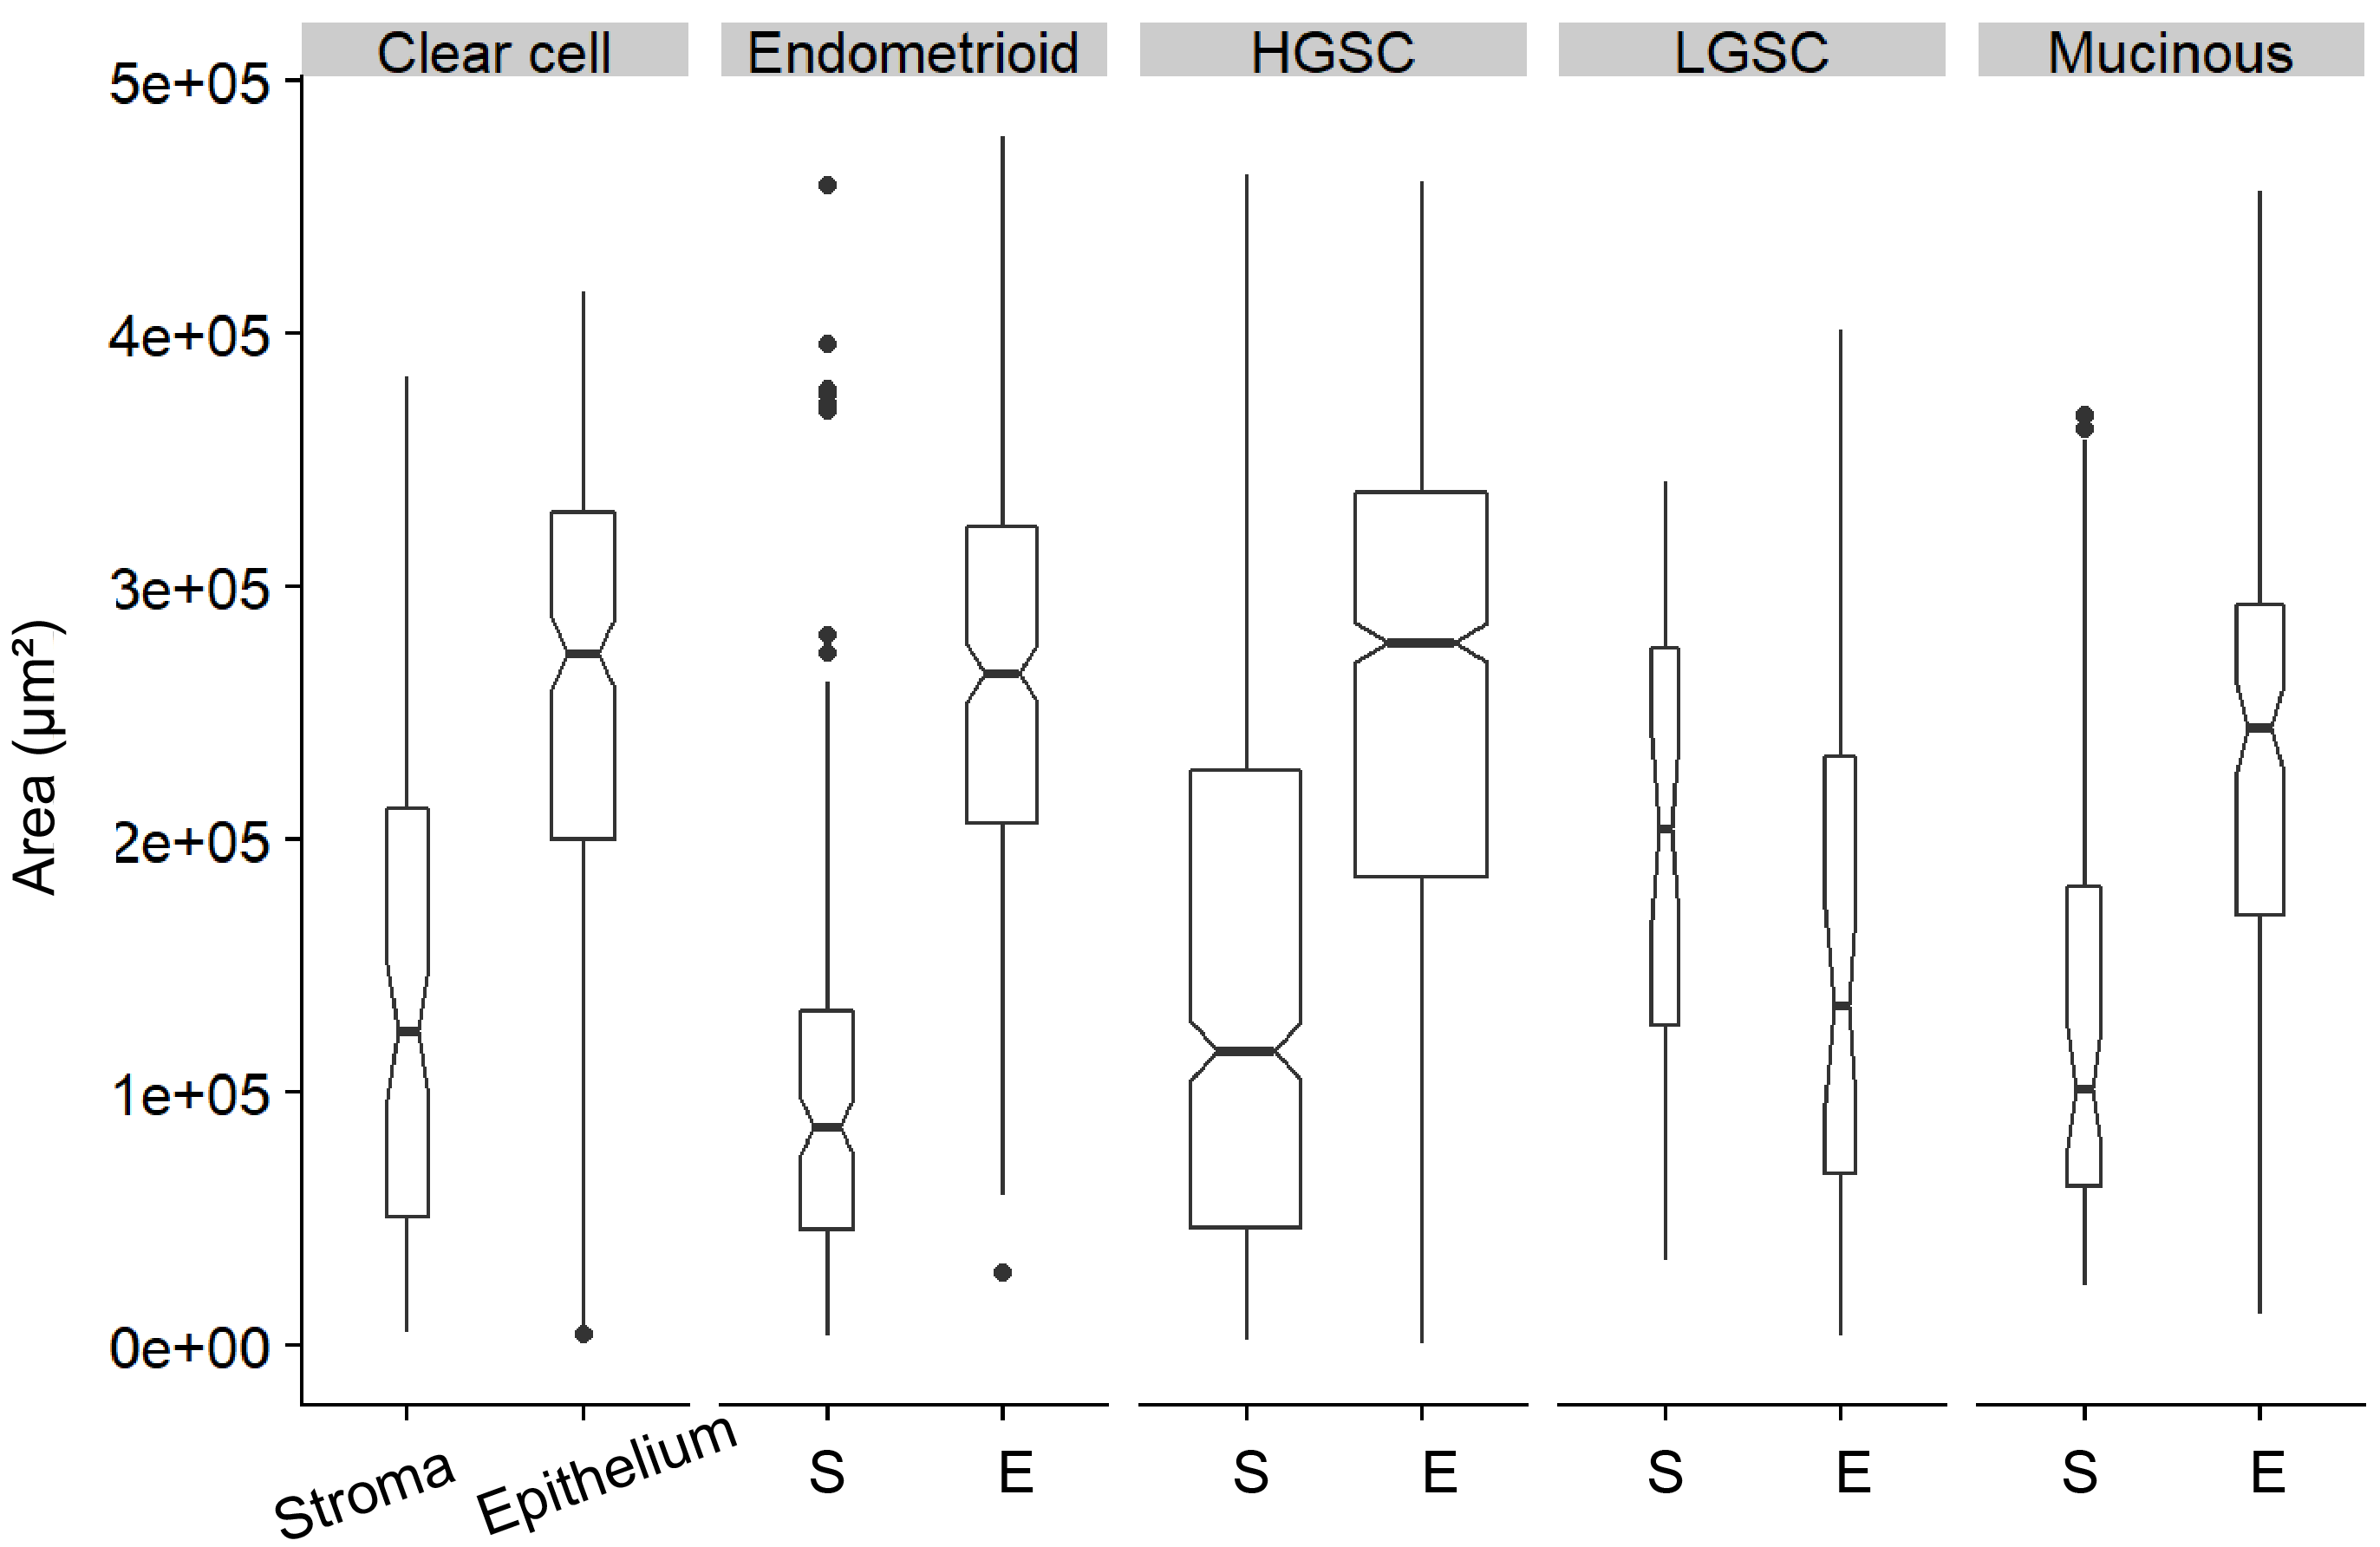
\includegraphics[width=0.8\textwidth]{Chapter2/Figs/Raster/Morphology_area.png}
    \caption{Area of tumour and stroma across morphological subtypes. (Notches on box plots extend 1.58 ✕ IQR / sqrt(n) and approximate the 95\% confidence interval for the median. Box plot whiskers extend to 1.5 ✕ IQR.) }
    \label{fig:morph_area}
\end{figure}

Figure \ref{fig:morph_immune} shows the distribution of CD45RO$^+$ cells in the stroma and epithelium across the different OC subtypes.

\begin{figure}
    \centering
    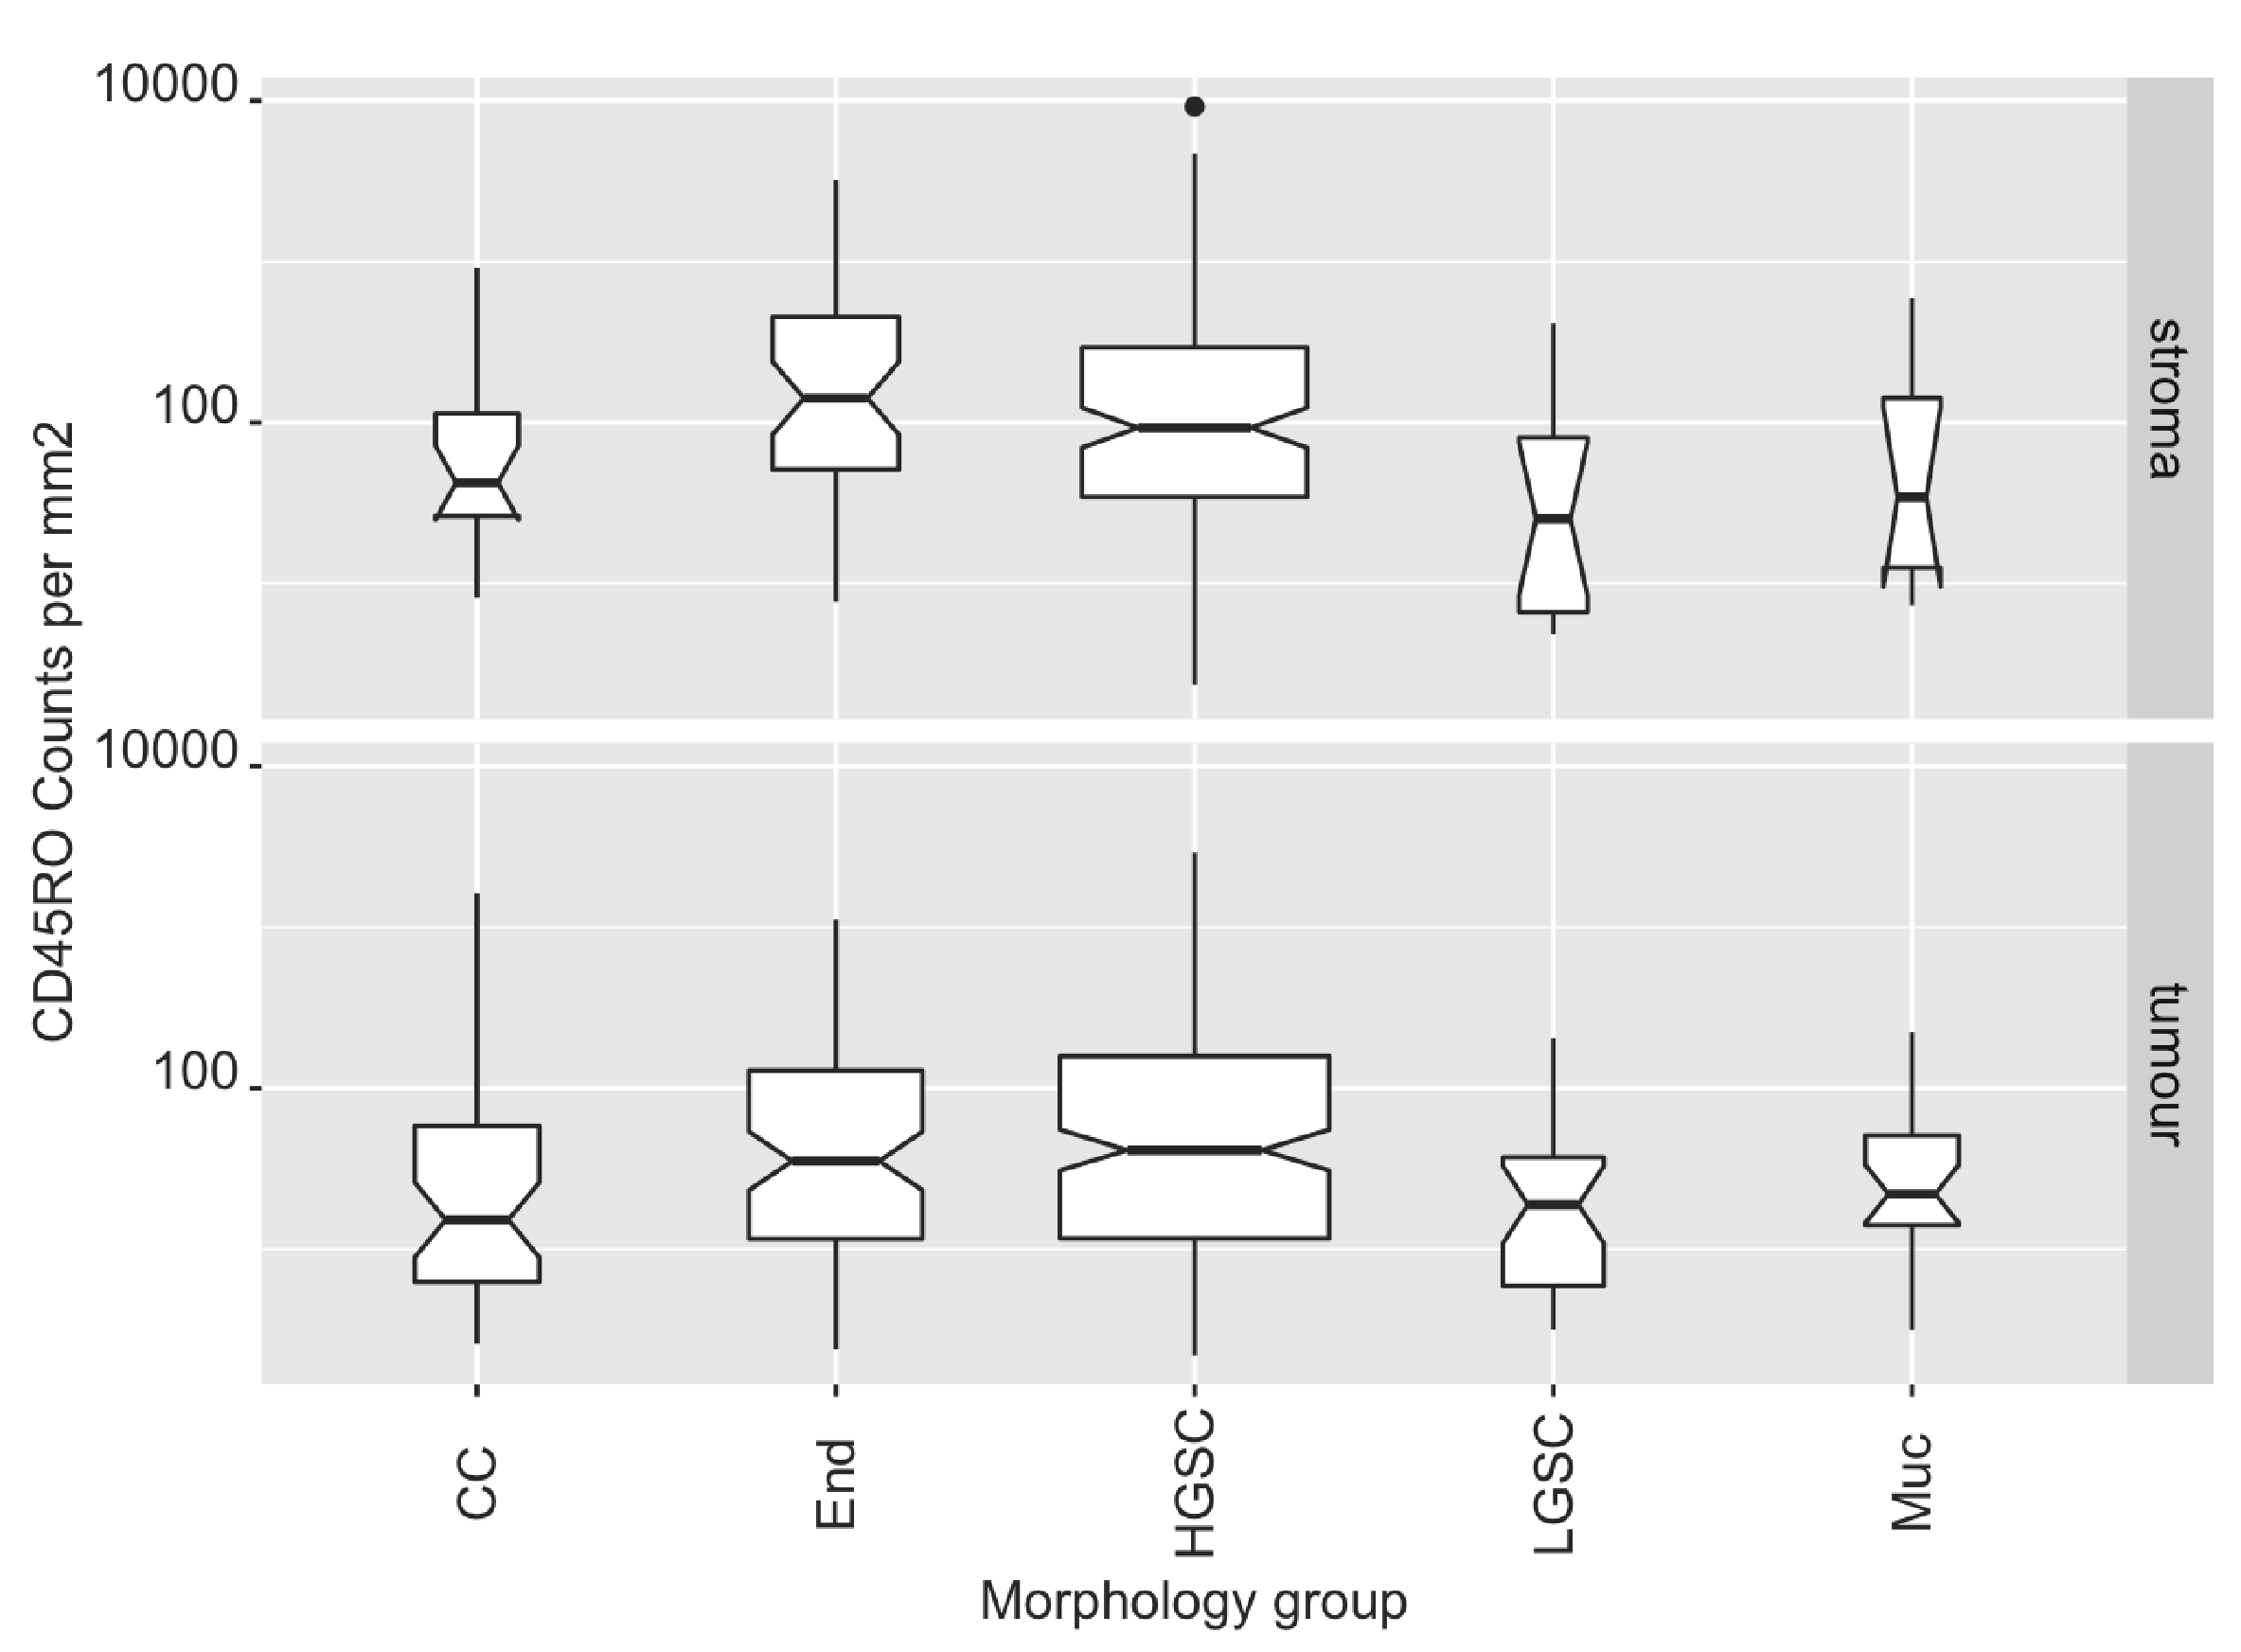
\includegraphics{Chapter2/Figs/Raster/CD45RO_morphology.png}
    \caption{Distribution of infiltrate in Stroma and Epithelium for different morphological subtypes of ovarian cancer. (Notches on box plots extend 1.58 ✕ IQR / sqrt(n) and approximate the 95\% confidence interval for the median. Box plot whiskers extend to 1.5 ✕ IQR.) }
    \label{fig:morph_immune}
\end{figure}

\clearpage

\section{Discussion}

The reproducible analysis of quantitative immune data allowed for a rigorous examination of the distributions of immune infiltrates within the SEARCH population and of the potential impacts of localisation of CD8+, CD68+ and CD45RO+ in HGSOC tumours. 

I observed in addition that stromal and epithelial populations and all infiltrates were somewhat positively correlated. This means that samples with low density of stromal immune populations generally had low density of epithelial infiltrate and vice versa. It also meant that patients with high quantities of one infiltrate type often had high infiltration of the others. It is worth noting that the  CD8$^+$ and  CD45RO$^+$ subpopulations are not biologically mutually exclusive and as such I expect some correlation between quantities but in this dataset there was no opportunity to examine the specific spatial locations of the immune cells. 

 One of the key and novel findings of this work was that the global measure of CD8$^+$ infiltrate was a stronger and more significant predictor of survival over CD8$^+$ infiltrate alone. The implication of the average infiltration being a stronger predictor of survival is that averaging over the intra-tumour stroma allows for a better measure of long term infiltration dynamics and measures the presence of a reservoir of immune cells, poised to infiltrate the epithelium.  I also demonstrated here that the quantity of epithelial and stromal CD45RO$^+$ is a positive prognostic feature, a result which also confirms the positive incremental benefit of a long term and mature immune response. 


As discussed in the introduction, many pieces of research have illustrated that macrophage function is micro-environment dependent\cite{ZhangMacrophage2014, li2018intratumoral}, demonstrating that exact localisation effects macrophage function. My work is in agreement with the observation by Li et al. that stromal regions are most prognostic in which to evaluate macrophages. I find however, in contrast to their work in lung cancer, that stromal CD68$^+$ macrophages are a positive prognostic feature. this is further evidence for distinct phenotypes of macrophages between tissue regions. The impact of specific immune cells can vary between cancer types and so further elucidation of the nature of macrophages in HGSOC and their interaction with the TME is required.


I investigated the concept of immune exclusion across this quantitative data set and found that the extent of exclusion was normally distributed. Such a distribution implies that there is not a one-directional process favouring exclusion. I found that the ratio of epithelial:stromal macrophages was prognostic, with increased epithelial macrophage:stroma macrophage ratio having a negative impact upon survival. I would have expected that the quantity of t-cell infiltration from the stromal to intra-epithelial regions would have effected tumour progression and hence survival but given this data I would assert that as the ratio is not prognostic and that the average of the t-cell subsets over the core is prognostic, that there is no explicit long term exclusion of cells, the infiltration at the tumour interface is dynamic and random and that the overall quantity in the larger region is more important than exclusion, which if it is an active process, was not observed to any extreme in this cohort.

Using quantitative data also allowed me see that there was no clear threshold for immune exclusion, but that a 10 fold difference in immune infiltration could be examined for comparisons. I observed that CD8$^+$,  CD45RO$^+$ and  CD68$^+$  infiltrates predominantly exist on a continuum without clear justification for cutpoints.

These observations all suggest that despite the focus of many studies being the intra-epithelial immune infiltration, perhaps due to a focus on direct contact and cytotoxic interaction between immune and tumour cells, that stromal infiltrate should also be evaluated, even in the case of CD8+ t-cell infiltration, to evaluate a larger area and obtain more accurate counts more easily. For macrophages it appears that stromal infiltration plays its own role in the immune response. In the case of the T-cell subsets evaluated here, the stromal region appears to provide more information about the epithelial infiltration as we can infer some element of the longer term immune infiltration dynamics.

In this chapter I also developed the concept of the immunospace. The immunospace views the quantity of each immune infiltration as part of a multidimensional immune landscape for a patient. This approach allowed me to analyse patterns across different immune populations and to derive the principal components as measures of variation. I observed that the correlation between infiltrates amounts to general coordinated immune response which is a positive prognostic. It also allowed me to examine the independence of other phenomenon such as the immune exclusion from the epithelium which was obtained as an axis of variation in an unbiased manner. Such high dimensional methods will be of importance when assessing higher dimensional data sets such as IMC. 


Having reduced the survival analysis to cores that contained epithelium and stroma in order to compare survival impact, the limitation of this analysis is that it assesses the impact of these immune cells within a stromally infiltrated environment. In order to address this I compared the survival impact of CD8 and CD45RO+ in the subset of cores with >99\% epithelium. CD45RO+ was no longer associated with survival which may imply a variation in the functionality of these cells which depends upon their spatial location (within tumour nest).

This work also finds no link between immune infiltration and germline \textit{BRCA} mutations, this is in part due to effects of cohort size. With approximately 20 patients with mutations, I am underpowered to ask multiple questions about the differences in immune infiltration between non-\textit{BRCA} and \textit{BRCA}-mutated patients.

The exact spatial nature of immune infiltration when taking into account tumour structure is unknown. There may also be a link between stromal immune infiltration and collagen deposition. Comparisons of immune infiltration to that which would be expected from diffusion into the epithelium alone has not been examined and is a key questions in the rest of this thesis.


%!TEX root = ../thesis.tex
%*******************************************************************************
%****************************** Third Chapter **********************************
%*******************************************************************************
\chapter{Quantifying and classifying tissue structure}

% **************************** Define Graphics Path **************************
\ifpdf
    \graphicspath{{Chapter3/Figs/Raster/}{Chapter3/Figs/PDF/}{Chapter3/Figs/}}
\else
    \graphicspath{{Chapter3/Figs/Vector/}{Chapter3/Figs/}}
\fi
\section{Introduction}
As shown in the previous section, stromal and epithelial immune infiltration may have differing roles within the response to a developing tumour. It is clear from observing image of tumour sections that the structure of the epithelium and stromal regions varies dramatically. These morphological differences have been discussed by Lisio et al. \cite{Lisio2019Feb} amongst others. This section of the thesis aims to set out an automated classification of such tissue structure, to investigate whether this can be reliably obtained from multiple types of tissue image and whether the structure defined this way is related to the infiltration of the tumour by particular types of immune infiltrate.  The workflow of this Chapter is illustrated in Figures \ref{fig:VA_ch4} and \ref{fig:VA_ch4_2}.

\begin{figure}
    \centering
    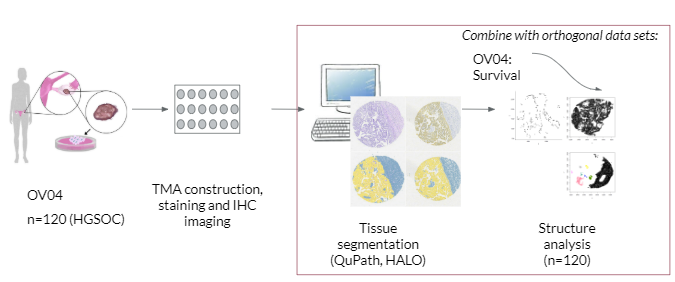
\includegraphics{Chapter3/Figs/Chapter3_VA.PNG}
    \caption{Visual Abstract for Chapter 4}
    \label{fig:VA_ch4}
\end{figure}

\begin{figure}
    \centering
    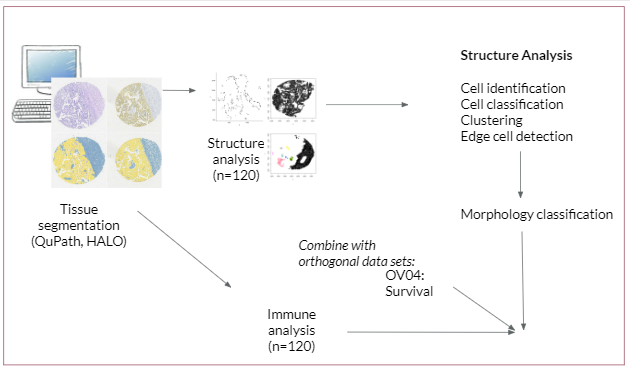
\includegraphics{Chapter3/Figs/VAch2_2.png}
    \caption{Visual Abstract for Chapter 4}
    \label{fig:VA_ch4_2}
\end{figure}

\section{Collaborators and Roles}
Sarwah Al-Khalidi(SAK) stained the OV04 TMA sections for CK7 and H&E.

\section{Methodology}
\subsection{Patient Cohorts}
Data from the OV04 Cohort was used for this section as it had existing sections that had H\&E and CK staining. This cohort also had sections available for further analysis using SHG. 

\subsection{IHC}
\subsubsection{Cytokeratin 7 staining}
Tissue sections from the OV04 cohort were stained with Cytokeratin7 by Sarwah Al-Khalidi and the method of staining and imaging is laid out in section \ref{sec:sarwah_staining}.

\subsection{H\&E}
Automated Haemotoxylin and Eosin staining was carried out by SAK and is described in \ref{sec:sarwah_staining}. 

\subsection{SHG}
SHG microscopy at wavelength 850nm was performed on the Leica SP5 microscope and imaged at 20x. DAKO mounting media and a coverslip of thickness 150um was used. 

\subsection{DBSCAN}
The package \textbf{dbscan} in R was used for density based clustering analysis. The mathematics of this method is discussed in the Methods. 

\section{Results}
Having found in the previous chapter that the specific localisation of several immune infiltrates was an important factor in the prognosis of patients, I wanted to investigate the structure of tissue sections and assess the impact of structure on immune infiltrate. I wanted to use both H&E and Cytokeratin stained images to derive this structure. Cytokeratin 7 was used as an epithelial marker to have a gold standard for structure analysis and to validate tissue classification of H\&E so that structures can be compared across multiple sections from the same core.

The morphologies discussed by Lisio et al are solid architecture, glandular architecture with slit-like spaces, papillary architecture and cribriform and pseudoendometroid architecture\cite{Lisio2019Feb} and in order to assess whether these structures could be automatically derived from images, the segmentation of tumour and stroma cells must first be acquired. 

\subsection{Patient Characteristics}
TMAs had been previously constructed from the CTCR-OV04 clinical studies, which were designed to collect imaging, blood, and tissue samples for exploratory biomarker studies. All patients provided written, informed consent for participation in these studies and for the use of their donated tissue, blood specimens, and anonymized data for the laboratory studies carried out. The CTCR-OV04 studies were approved by the Suffolk Local Research Ethics Committee (reference 05/Q0102/160) and Cambridgeshire Research Ethics Committee (reference 08/H0306/61).\cite{}

The TMA previously constructed for this cohort contained 40 patients with HGSOC. 

\begin{table}[]
    \centering
    \begin{tabular}{c|c}
       N  &  40 \\
        Age &  77 (60-90)
    \end{tabular}
    \caption{OV04 study patient characteristics}
    \label{tab:OV04_patient}
\end{table}




\subsection{Cell classifier performance and comparison between H\&E and CK}

Images of tissue sections stained with both H\&E and a CK7 marker were analysed. QuPath was used to segment nuclei based upon their optical density. Nuclei were then classified based upon features using a random forest based classifier. Cells were split randomly into a test and training data set. Examples of tissue classification on H\&E and CK stained images. Over 5000 cells from each TMA section were labelled and 70\% were used for training and 30\% were used for validation test sets. Confusion matrices for the H\&E and CK classifier are shown in Tables (\ref{tab:classifier_he} and \ref{tab:classifier_ck}). These show a very good performance by both classifiers. 


\begin{figure}
    \centering
    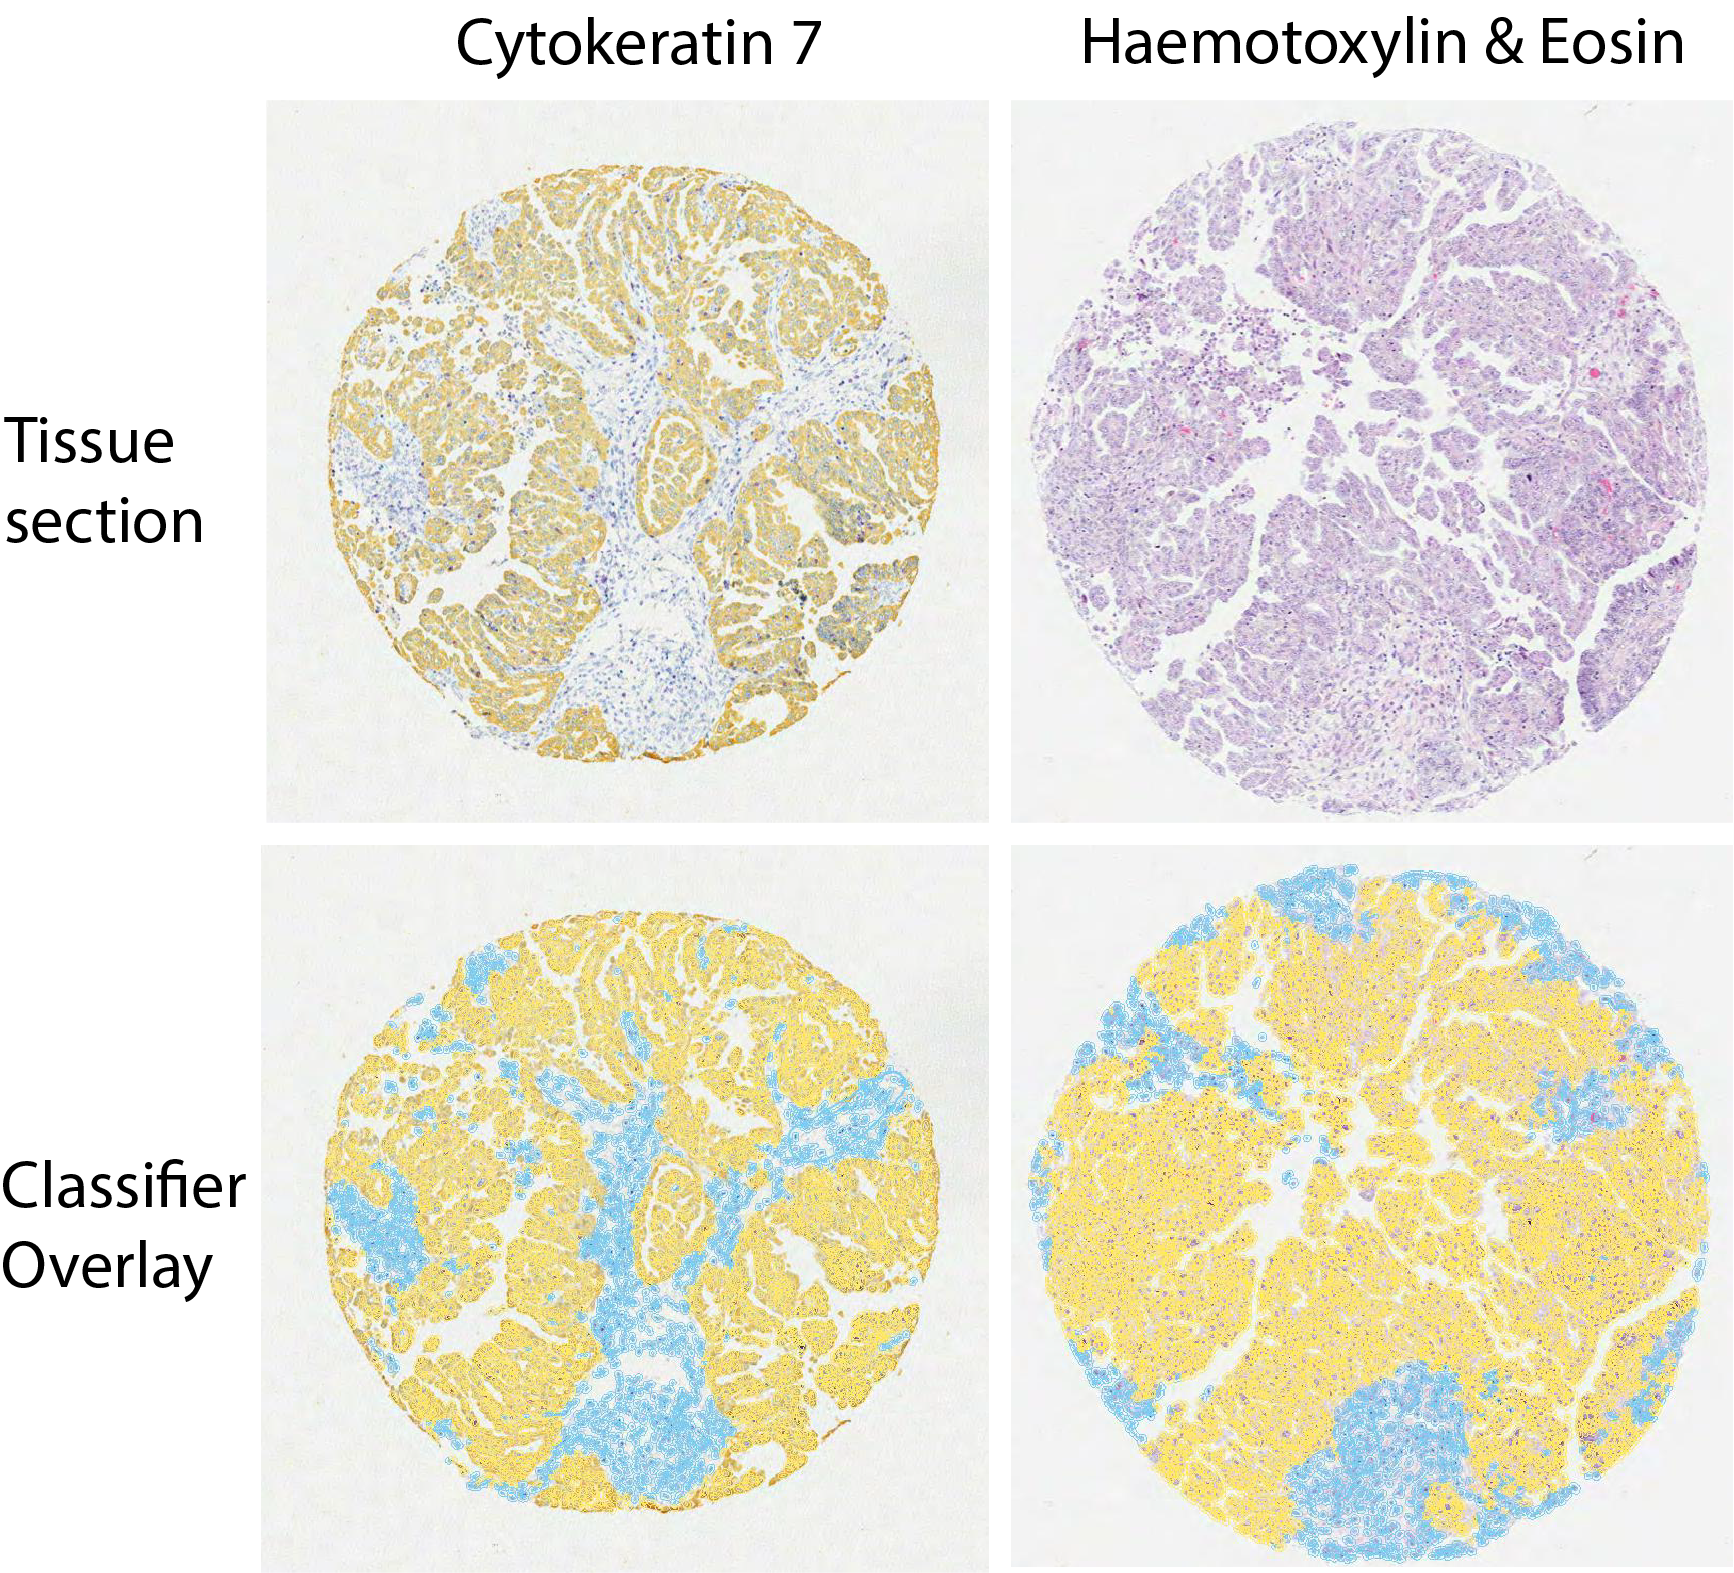
\includegraphics{Figs/heck/A-2_core_class.png}
    \caption[Example of Stroma and Tumour classifier built in QuPath software]{Example of Stroma and Tumour classifier built in QuPath software. Tumour is highlighted in yellow and stroma in blue. Classifier is trained on both H\&E and CK7 stained images.}
    \label{fig:he_classify}
\end{figure}

\begin{table}[]
    \centering
    \begin{tabular}{l|cc}
       &   Stroma  &   Tumor\\
       \hline
Stroma   &    1263    &     2\\
Tumor   &      2     &  346 \\
         
    \end{tabular}
    \caption[Confusion matrix for QuPath CK based classifier.]{Confusion matrix for QuPath CK based classifier. Classifier accuracy is 98.75\% (n=1613).}
    \label{tab:classifier_ck}
\end{table}


\begin{table}[]
    \centering
    \begin{tabular}{llcc}
    \hline
       &           &  Label &\\
       &           &    Stroma	& Tumor\\ 
\hline
Classification & Stroma	&  2653	 &   40\\
             & Tumor	 &   11	 & 2165\\
 \hline
    \end{tabular}
    \caption[Confusion matrix for QuPath H\&E based classifier.]{Confusion matrix for QuPath H\&E based classifier. Percentage of correctly classified objects in test set: 98.95\% (n=4869).}
    \label{tab:classifier_he}
\end{table}


\subsection{High Grade Serous tissue structure analysis}

In order to define a tissue structure of each core I selected several properties to examine and measure;

\begin{itemize}
    \item Stroma/Tumour percentage
    \item Surface Area: Volume ratio
    \item Cellular entropy
    \item Number of clusters 
\end{itemize}

\subsubsection*{Stroma/Tumour percentage}
This most basic measure of tissue composition was utilized in the previous chapter. In this chapter I measured this percentage as both an area and a number proportion for each image type. Figure\ref{fig:correlation_tumourarea} shows that the two values are strongly correlated as would be expected from serial sections. 

\begin{figure}
    \centering
    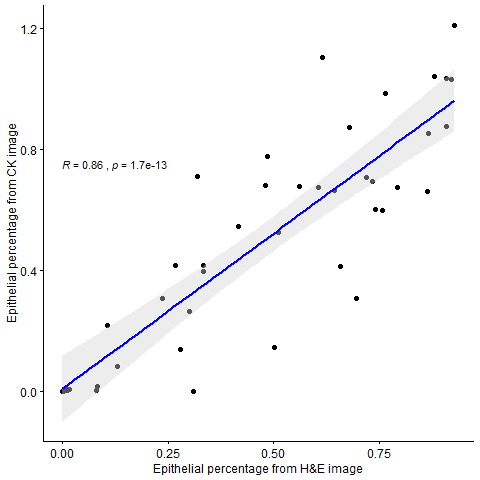
\includegraphics[width=0.5\textwidth]{Chapter3/Figs/correlation_TS_he_Ck.png}
    \caption{Correlation between percentage epithelium measured via H&E and that measured by analysis of an image of a CK stained serial section.}
    \label{fig:correlation_tumourarea}
\end{figure}

\subsubsection*{Invasive front}
In a purely diffusive model where immune infiltrate travels from the stroma into the epithelial nests, epithelial infiltrate would be proportional to the surface area of the epithelial nodules that are exposed to the surrounding stroma. In order to gain a measure of this surface area, I defined edge cells as those cells which had a nearest neighbour of a differing class. The surface area to volume ratio can be estimated in 2D as 
\begin{equation}
    
\frac{N_{edge cells}}{N_{\mathrm{epithelial}}}
\end{equation}

\begin{figure}
    \centering
    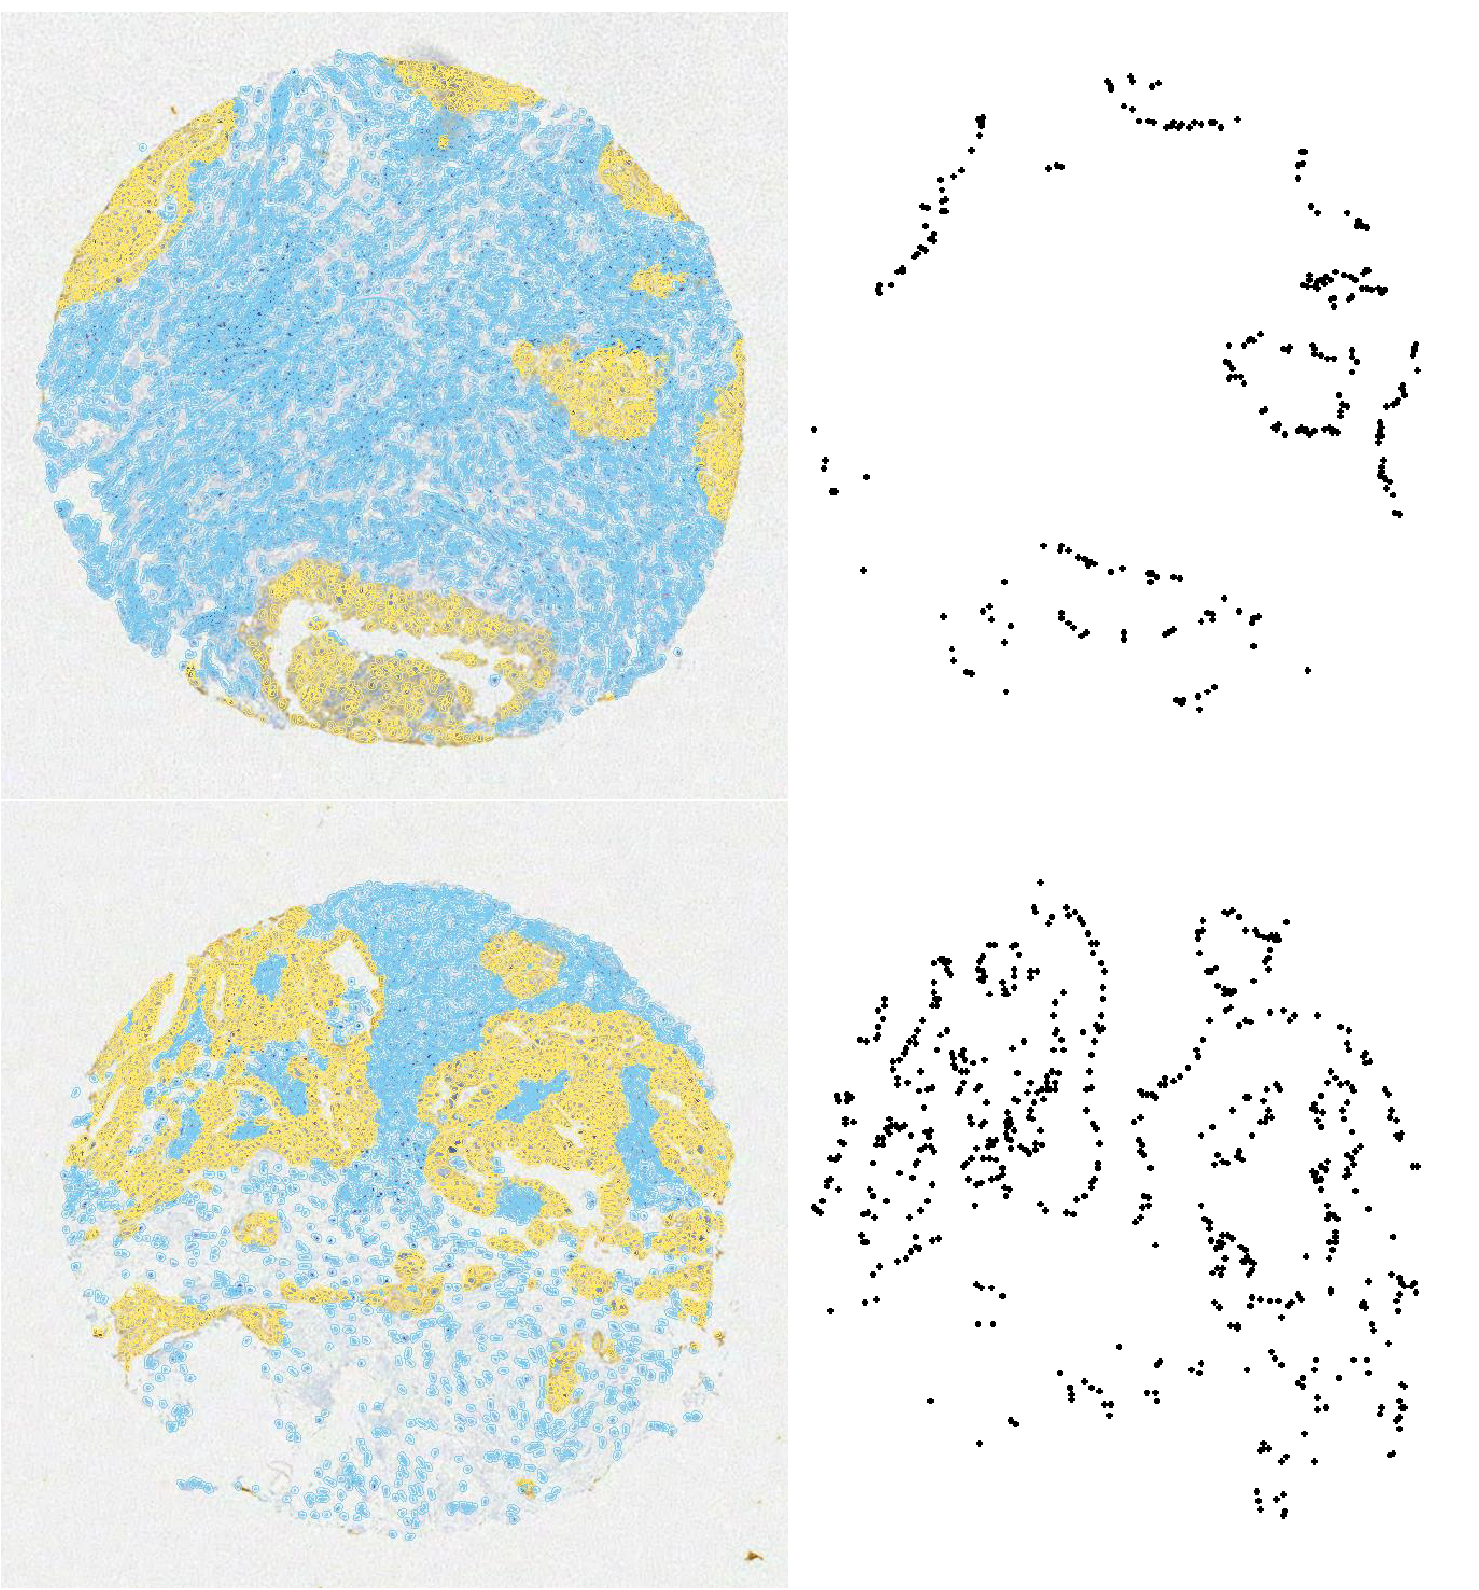
\includegraphics[width=0.5\textwidth]{Chapter3/Figs/Thesis-08.png}
    \caption{Example of classified images (left) and the cells in the image designated as edge cells(right).}
    \label{fig:edge_cells}
\end{figure}

\subsubsection*{Clustering}
I assessed multiple methods for clustering tissues, in terms of identifying groups of tissues I found that it was best to use DBSCAN, a density based clustering method. The results of other clustering methods are shown in \ref{fig:clust_bad}. An example of DBSCAN on serial H\&E and CK sections are show in Figure \ref{fig:dbclust}. These show very similar identifications of clusters across both samples.

\begin{figure}
    \centering
    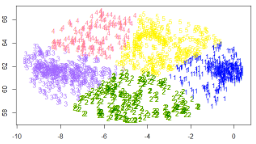
\includegraphics{Chapter3/Figs/knn_example_2.png}
    \caption[k-nearest neighbour clustering of cells]{k-nearest neighbour clustering of cells identified in a tissue section. The requirement of a pre-specified number of clusters and that the algorithm does not account for varying density or information other than nearest neighbours, means that this method of clustering fails to automatically identify good clustering and in the case of densely packed TMA sections will merely split it equally.}
    \label{fig:clust_bad}
\end{figure}

\begin{figure}
    \centering
    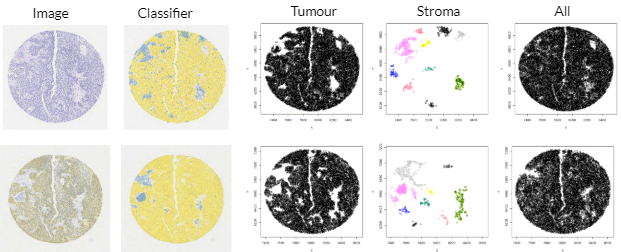
\includegraphics[width=\textwidth]{Chapter3/Figs/dbscan_fullexample.png}
    \caption{Examples of clusters of cells within tissue sections when epithelial, stromal cells are viewed separately and when all cells are clustered.}
    \label{fig:dbclust}
\end{figure}

\begin{figure}
    \centering
    \includegraphics{}
    \caption{Number of clusters.}
    \label{fig:dbscatter}
\end{figure}

\subsubsection*{Entropy}
In addition to the number of stromal and tumour clusters, I wanted to add entropy at multiple scales to the tissue features. Entropy can be understood as a measure of mixing and the formula for deriving entropy is given in Methods \ref{eq:entropy}. I hypothesised that given that tissue regions with mixed cell types would have a higher entropy than those without, that with multiscale area sampling, a reliable classification into tumours with mixing and without could be achieved. Figure \ref{fig:entropy} gives the mean entropy over 20 subsections of the image for matched H\&E and CK stained sections. This shows a moderate correlation but. 

\begin{figure}
    \centering
    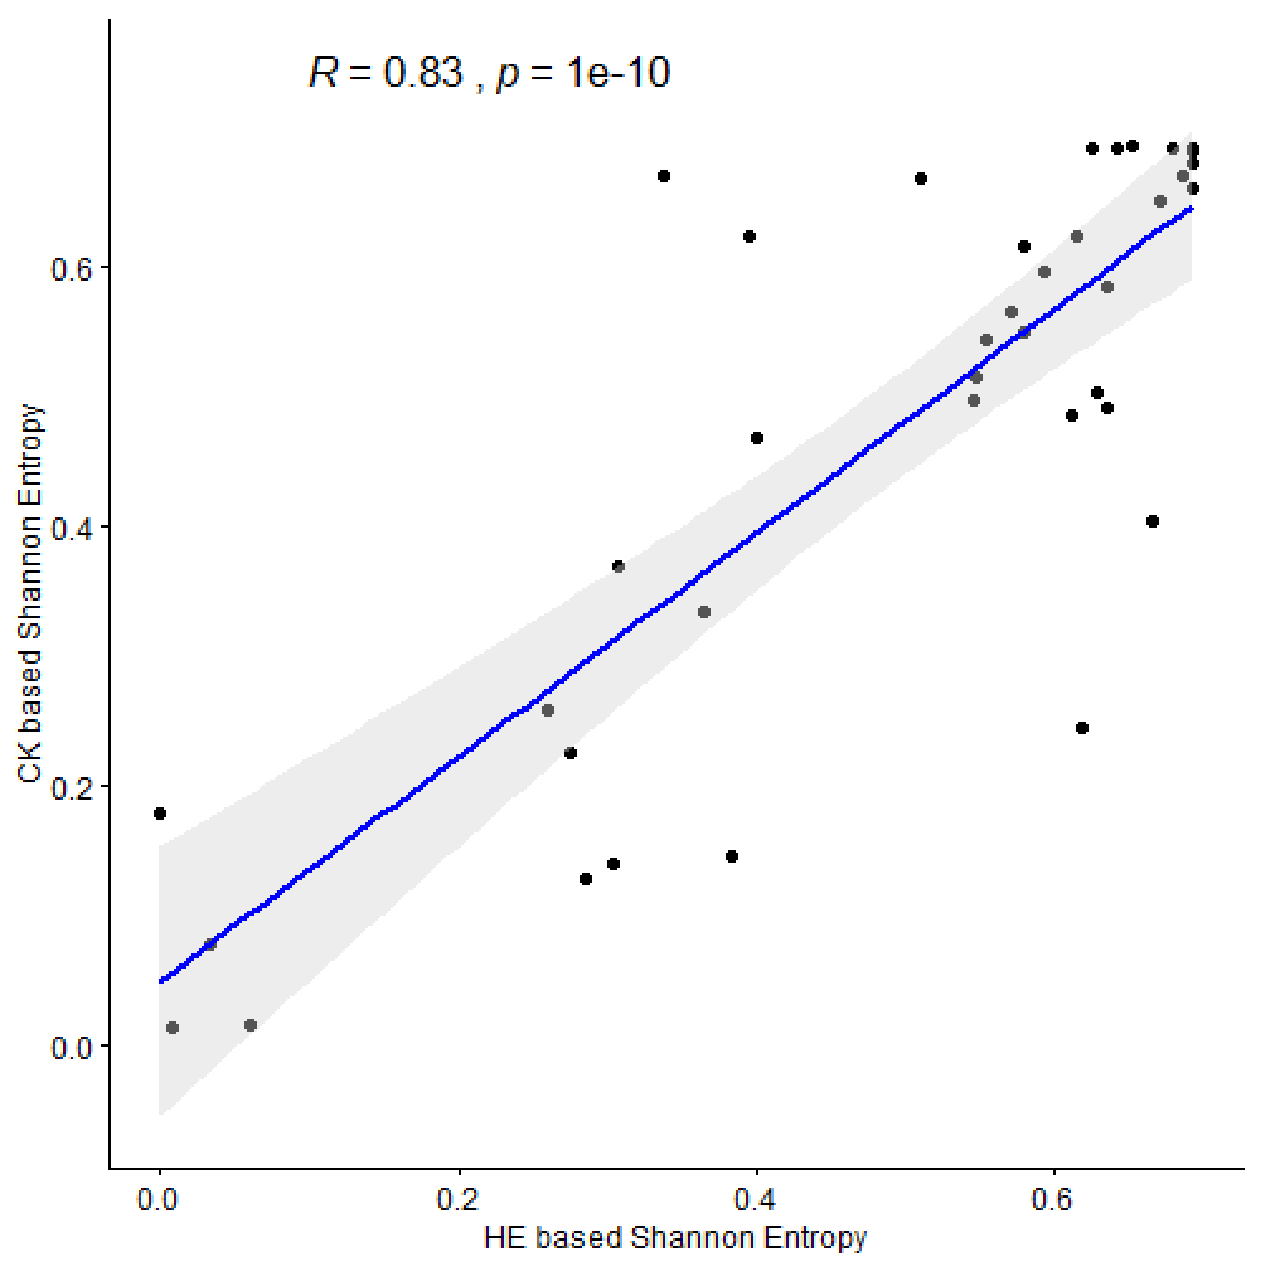
\includegraphics{Chapter3/Figs/Thesis-06.png}
    \caption{Shannon entropy derived for a H\&E and CK image of serial sections from the same patient core.}
    \label{fig:entropy}
\end{figure}

\subsection{Morphology classification}
Having reliably identified stromal and epithelial cells and identified subclusters and entropy of tissue I aimed to then classify tissue sections based upon these features into the morphological subtypes mentioned earlier.

In order to do this I labelled each tissue section as Solid, Glandular or Unknown.
\begin{figure}
    \centering
    \includegraphics{}
    \caption{Histogram of the number of cases classified as solid, glandular, epithelial  or cribriform structure.}
    \label{fig:num_classl}
\end{figure}

\subsection{Relationship between Structure and Immune infiltration}

\subsubsection{Immune quantification}

CD8 and FOXP3 were assessed in OV04 samples.
\begin{itemize}
    \item Correlation between CD8, FOXP3 and edge cells
    \item Immune cells for different structures
\end{itemize}

\subsection{Speed/Quantity model}

\subsection{Collagen structure analysis}

\section{Discussion}


In spite of multiple data sources implying a continuous distribution of densities of infiltration of immune cells into tumours, the literature still dichotimises immune infiltrate and even categorises a subclass of tumour structures as immune reactive, an approach which fails to interpret that differences in structure may influence the immune cells which can infiltrate and the rate at which they do.

I found that the number of X was correlated with immune infiltrate. 

%!TEX root = ../thesis.tex
%*******************************************************************************
%****************************** Fourth Chapter *********************************
%*******************************************************************************

\chapter{Colocalisation of immune infiltrates and spatial statistics of immune cell-tumour-stroma interaction}

\ifpdf
    \graphicspath{{Chapter4/Figs/Raster/}{Chapter4/Figs/PDF/}{Chapter4/Figs/}}
\else
    \graphicspath{{Chapter4/Figs/Vector/}{Chapter4/Figs/}}
\fi


\section[Introduction]{Introduction}

As mentioned in the introduction, some methods of immune analysis are capable of measuring many more markers on a single section than standard IHC and IF. IMC is one of the best of such methods, allowing for measuring more than 20 markers on a single tissue section by conjugating antibodies with metal isotopes. This method allowed me to view additional markers for microenvironmental features such as collagen and hypoxia alongside a panel of immune markers that had been investigated in other samples. In order to investigate the micro-environment in both epithelium and the tumour-adjacent stroma I used the BriTROC and ICON7 cohorts to investigate this.

\subsection{History of the project and roles}
Sarwah Al-Khalidi originally intended to create an IMC panel for immune markers alone, I worked with SAK to include collagen in order to both better delineate stroma tissues from epithelium and investigate the structure of collagen and its interaction with immune cells. Sarwah Al-Khalidi (SAK) carried out the panel optimization and staining on the BriTROC cohort and arranged for Fatime Cosaj(FC) to carry out the staining with the same panel on the ICON7 cohort using the same protocols as optimized by SAK. I arranged for Richard Grenfell (RG) to carry out the imaging of the stained ICON7 slides on the same machine as the BRITROC cohort had been done.

From the markers included in the IMC panel, the subset of these of markers that I was interested in were;
\begin{itemize}
\item \textbf{CD8, CD68, CD45RO, FOXP3} - Key immune cell populations for comparison with other datasets
\item \textbf{CK7, Collagen1} - Key structural markers, gold standards for comparison of epithelial structure and quantity with other datasets
\item \textbf{CA9} - Hypoxia marker to investigate the relationship between tissue structure and hypoxia
\item \textbf{Ki-67} - Proliferation marker to investigate the relationship between tissue structure and proliferation \end{itemize}

\begin{figure}
    \centering
    \includegraphics{}
    \caption{Visual abstract for this chapter. IMC images are processed and collagen channels as well as multi-immune channels are cleaned and then analysed for structural and spatial features.}
    \label{fig:ch5_visualabstract}
\end{figure}

\section[Methodology]{Methodology}
\subsection{Cohort Summary}
\subsubsection{BriTROC} Samples were collected previous to this PhD under the British Translational Research Ovarian Cancer Collaborative (BriTROC), a non-randomised prospective study enrolling patients with recurrent HGSOC\cite{}.  Figure \ref{fig:BriTROC_remark} shows the REMARK diagram for this cohort. A total of 446 diagnostic samples were collected from 276 patient with relapsed HGSOC. 247 samples from 172 patients had enough material to generate a tissue microarray (TMA) for immunohistochemistry staining. Three 1mm cores from the tumour area of each sample were marked on H&E-stained slides by a pathologist, and used by Darren Ennis to make a tissue microarray (TMA) of the samples.
\begin{figure}
    \centering
    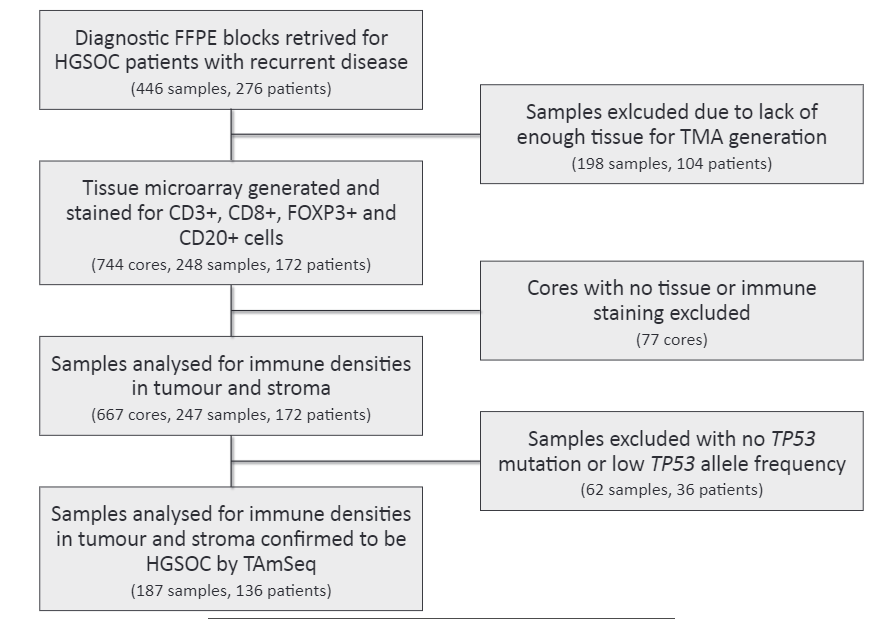
\includegraphics{Chapter4/figs/remark_britroc.png}
    \caption{REMARK diagram for the BriTROC cohort.}
    \label{fig:BriTROC_remark}
\end{figure}


\subsubsection{ICON7}
ICON7 was an international, phase 3, open-label, randomised trial undertaken at 263 centres in 11 countries across Europe, Canada, Australia and New Zealand. Eligible adult women with newly diagnosed ovarian cancer that was either high-risk early-stage disease (International Federation of Gynecology and Obstetrics [FIGO] stage I–IIa, grade 3 or clear cell histology) or more advanced disease (FIGO stage IIb–IV), with an Eastern Cooperative Oncology Group performance status of 0–2, were enrolled and randomly assigned in a 1:1 ratio to standard chemotherapy (six 3-weekly cycles of intravenous carboplatin [AUC 5 or 6] and paclitaxel 175 mg/m2 of body surface area) or the same chemotherapy regimen plus bevacizumab 7·5 mg per kg bodyweight intravenously every 3 weeks, given concurrently and continued with up to 12 further 3-weekly cycles of maintenance therapy. Randomisation was done by a minimisation algorithm stratified by FIGO stage, residual disease, interval between surgery and chemotherapy, and Gynecologic Cancer InterGroup group. The primary endpoint was progression-free survival; the study was also powered to detect a difference in overall survival. Analysis was by intention to treat. This trial is registered as an International Standard Randomised Controlled Trial, number ISRCTN91273375\cite{Perren2011Dec, BibEntry2020Jan}. Figure \ref{fig:icon_remark} is a REMARK diagram of samples analysed. TMA prepared by MRC.

ICON7 had cores sampled specifically from Epithelium and adjacent stroma, making it ideal for measurement of the microenvironment and measurement of both tumour and stroma in a single section which had been limited to a subset of the patients in previous cohorts.

\subsection{Immuno Metal Conjugation}
The protocol for IMC staining and imaging was carried out as described in Section \ref{sec:sarwah_staining}.

\subsection{Marker Panel}
The marker panel is specified in section \ref{table:imc_antibodies} and I worked with SAK to include Collagen in this panel for further investigation alongside the immune populations. 


\subsection{Staining and Imaging}
Staining and imaging of the BriTROC panel was carried out by SA-K. Staining and imaging of the ICON7 TMAs was carried out by Fatime Cosaj(FC) and Richard Grenfell(RG) accordingly.

\subsection{Image Analysis}
Python was used for data cleaning and Halo was used for the subsequent analysis of IMC data files. Structure analysis of signal in the collagen channel was carried out with Imagej and the GLCM, Orientationj and Directionality plugins. 


\section{Results}
Before analysing the interaction between these immune cells and these single populations on single tissue sections, I investigated the characteristics of the BriTROC and ICON7 cohorts are shown.

\subsection{BriTROC summary}
\subsection{ICON7 summary}
There were X patients.

\subsection{IMC image analysis}
 IMC images contain hot pixels distributed randomly across the image, in order to clean the data, I carried out hot-spot removal in python using a median filter with a 3x3 pixel area (see Code \ref{script:1}).
 
 I built a classifier in Halo to distinguish epithelial tissue from low density and high density collagen, specified by the intensity of the Collagen1 marker over small areas.
 I then built cell segmentation algorithms based on nuclear DNA marker staining to segment nuclei. I then used the IMC marker panel to classify cells based on their nuclear and cytoplasmic staining. An example of tissue segmentation and cell segmentation and classification of ICON7 and BRITROC image is shown in Figure \ref{fig:IMC_example}.
 
 \begin{figure}
     \centering
     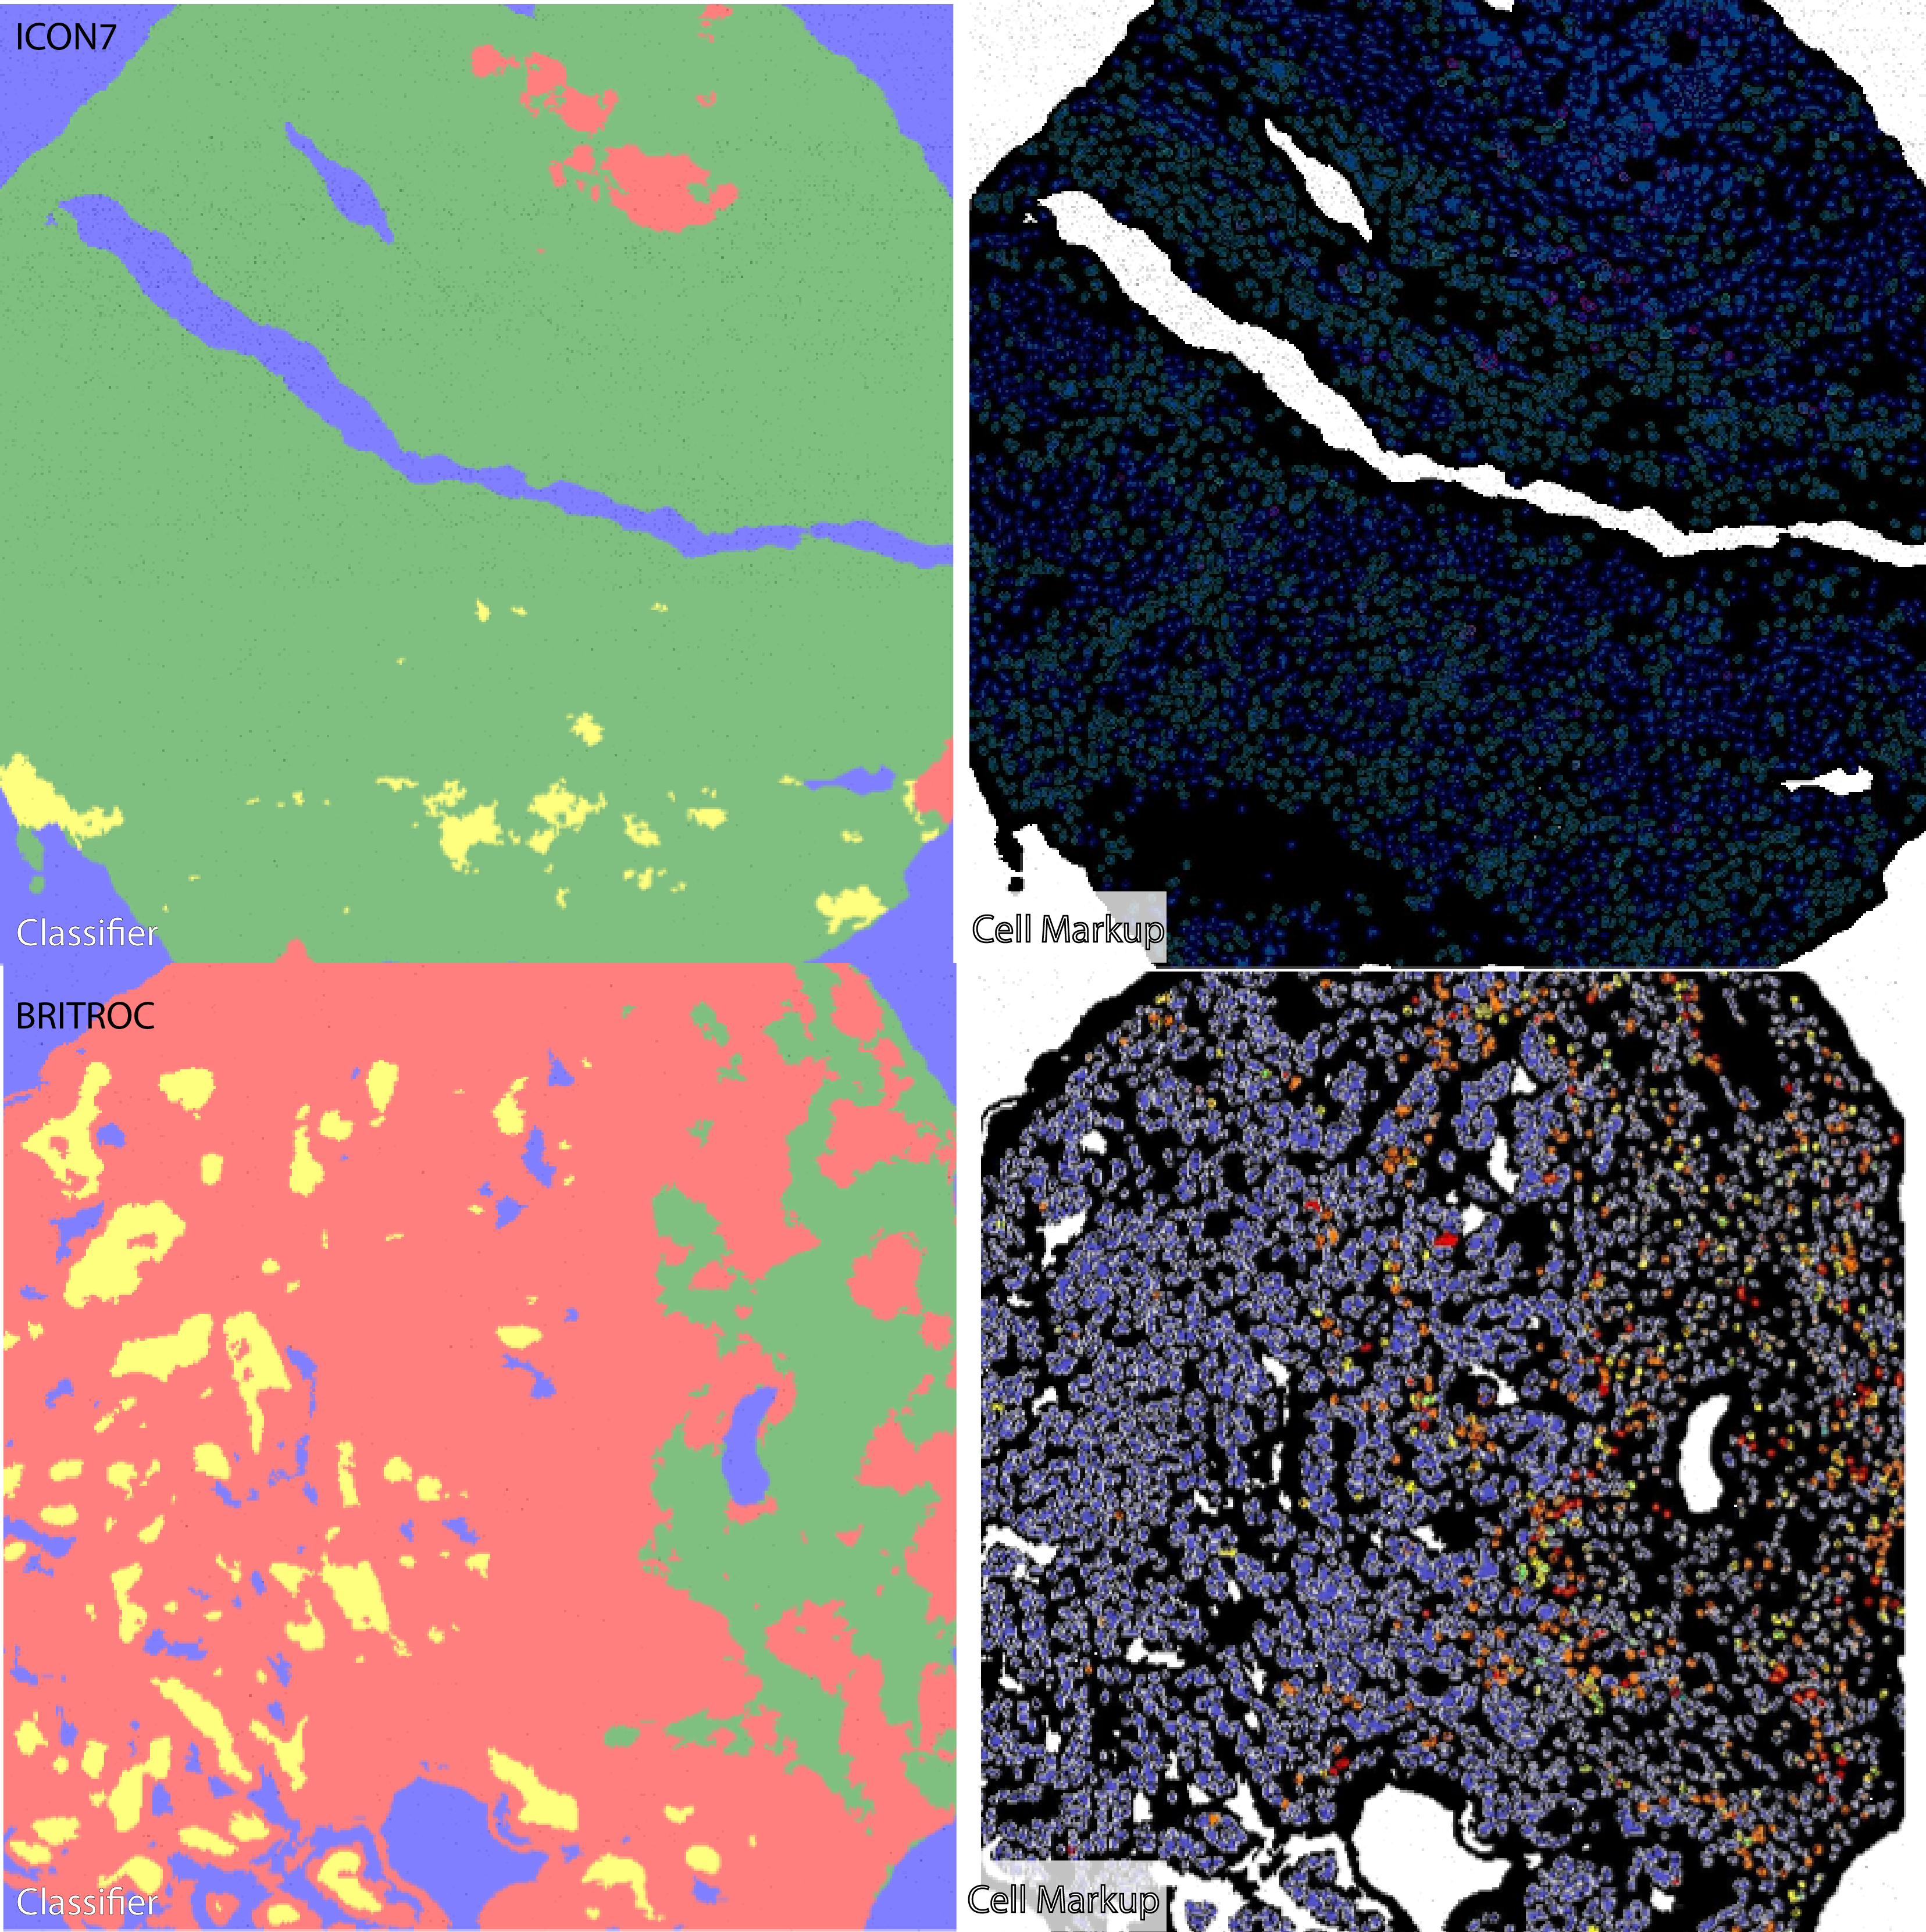
\includegraphics[width=0.5\textwidth]{Chapter4/figs/Thesis-09.png}
     \caption{Example of BRITROC and ICON7 classifier region and cell markup from HALO on IMC images.}
     \label{fig:IMC_example}
 \end{figure}
 
\subsubsection{IMC validation}

In order to validate the tissue and cell classification of the IMC, I used multiplexed IHC from serial sections of the same cohort to compare. Figure \ref{fig:IMC_IHC_corr} shows the correlation between IHC and IMC derived CD8/CD68 and between IMC and IHC derived stroma/tumour quantities.

\begin{figure}
    \centering
    \includegraphics{corr_IMC}
    \caption{Correlation between the epithelium quantity, CD8 cell density and CD68 cell density as measured in IHC and IMC on the BRITROC cohort.}
    \label{fig:IMC_IHC_corr}
\end{figure}

\subsection{Exploratory data analysis of TMA1}

The BRITROC cohort composed 3 TMAs in triplicate, I decided to use the first TMA in order to do an exploratory analysis for hypothesis generation. I would then be able to test the statistical significance of such hypotheses on both the other two TMAs and the ICON7 cohort. 

The first exploratory investigation of this dataset was to investigate the correlations between immune populations to validate the results found in earlier chapters and to build up a picture of which features of the micro-environment are connected.

I first investigated the correlation between numbers of CD3, CD8 and PD-1 positive cell areas in samples.

\begin{figure}
    \centering
    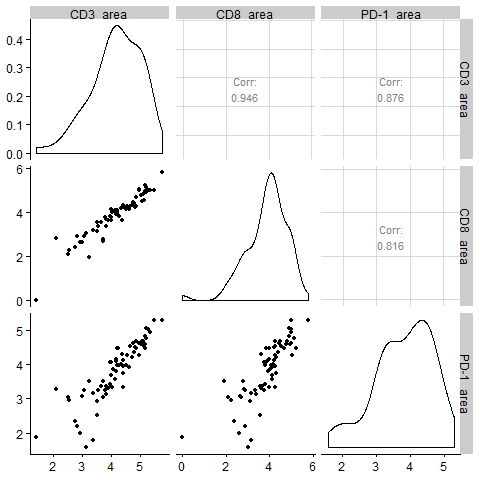
\includegraphics[width=0.5\textwidth]{Chapter4/figs/BRITROC_CD3_CD8_PD-1_corr.png}
    \caption{CD3, CD8, PD-1}
    \label{fig:CD8_CD3_PD1}
\end{figure}

\begin{figure}
    \centering
    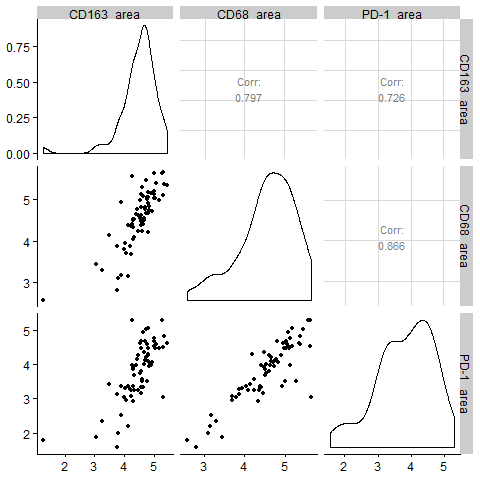
\includegraphics{Chapter4/figs/BRITROC_CD163_CD68_PD-1_corr.png}
    \caption{CD163, CD68, PD-1}
    \label{fig:CD163_CD8_PD1}
\end{figure}

\begin{figure}
    \centering
    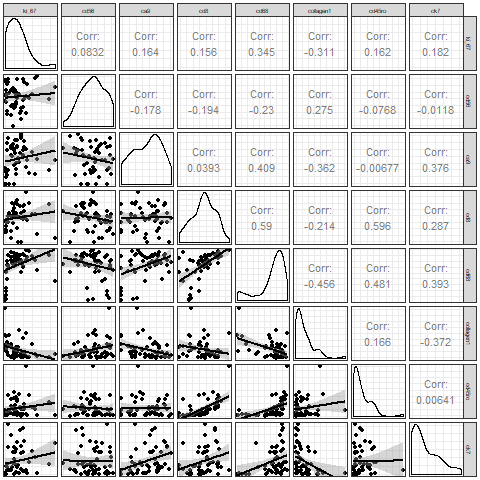
\includegraphics{Chapter4/figs/Britroc_cell_correlation2.png}
    \caption{Scatterplots of correlations between number of cells positive for each marker.}
    \label{fig:britroc_corr_scatt}
\end{figure}

\begin{figure}
    \centering
    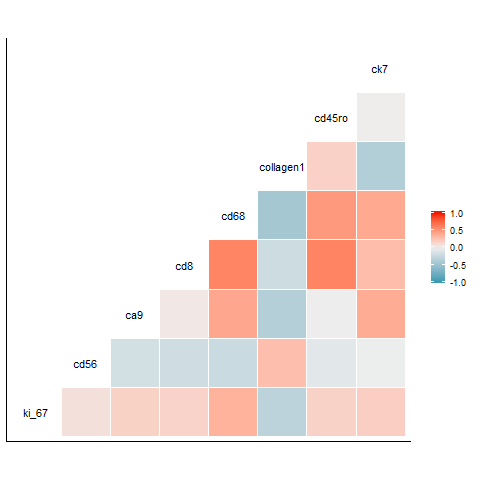
\includegraphics[width=0.5\textwidth]{Chapter4/figs/Britroc_cell_correlation.png}
    \caption{Heatmap of correlations between number of cells positive for each marker.}
    \label{fig:britroc_corr_heat}
\end{figure}

Figures \ref{fig:britroc_corr_scatt} and \ref{fig:britroc_corr_heat} show the correlations between the number of CD8+, CD68+, CA9, CK7, Collagen1, CD45RO, CD56 and Ki-67+ cells. CD8, CD68 and CD45RO, the populations investigated in Chapter 1, show the strongest positive correlations. I also see the negative correlation we would expect between the number of Collagen and Cytokeratin positive cells as these cells are mutually exclusive and determine the majority of the structure of a tissue. Despite seeing a higher density of infiltrate in stromal regions in earlier chapters, we see a negative correlation between the number of collagen positive cells and the number of immune cells in these samples.

\subsection{Principal Component Analysis}
In order to carry out a meaningful analysis across such a large number of measurements in multiple tissue regions, I used principal component analysis as in Chapter 2 in order to examine the patterns across the immune infiltrates. 

\subsection{Comparing immune cell densities between epithelium, high density and low density collagen}

\subsubsection{Macrophages}

CD68 and CD163 are both macrophage markers. 

\begin{figure}
    \centering
    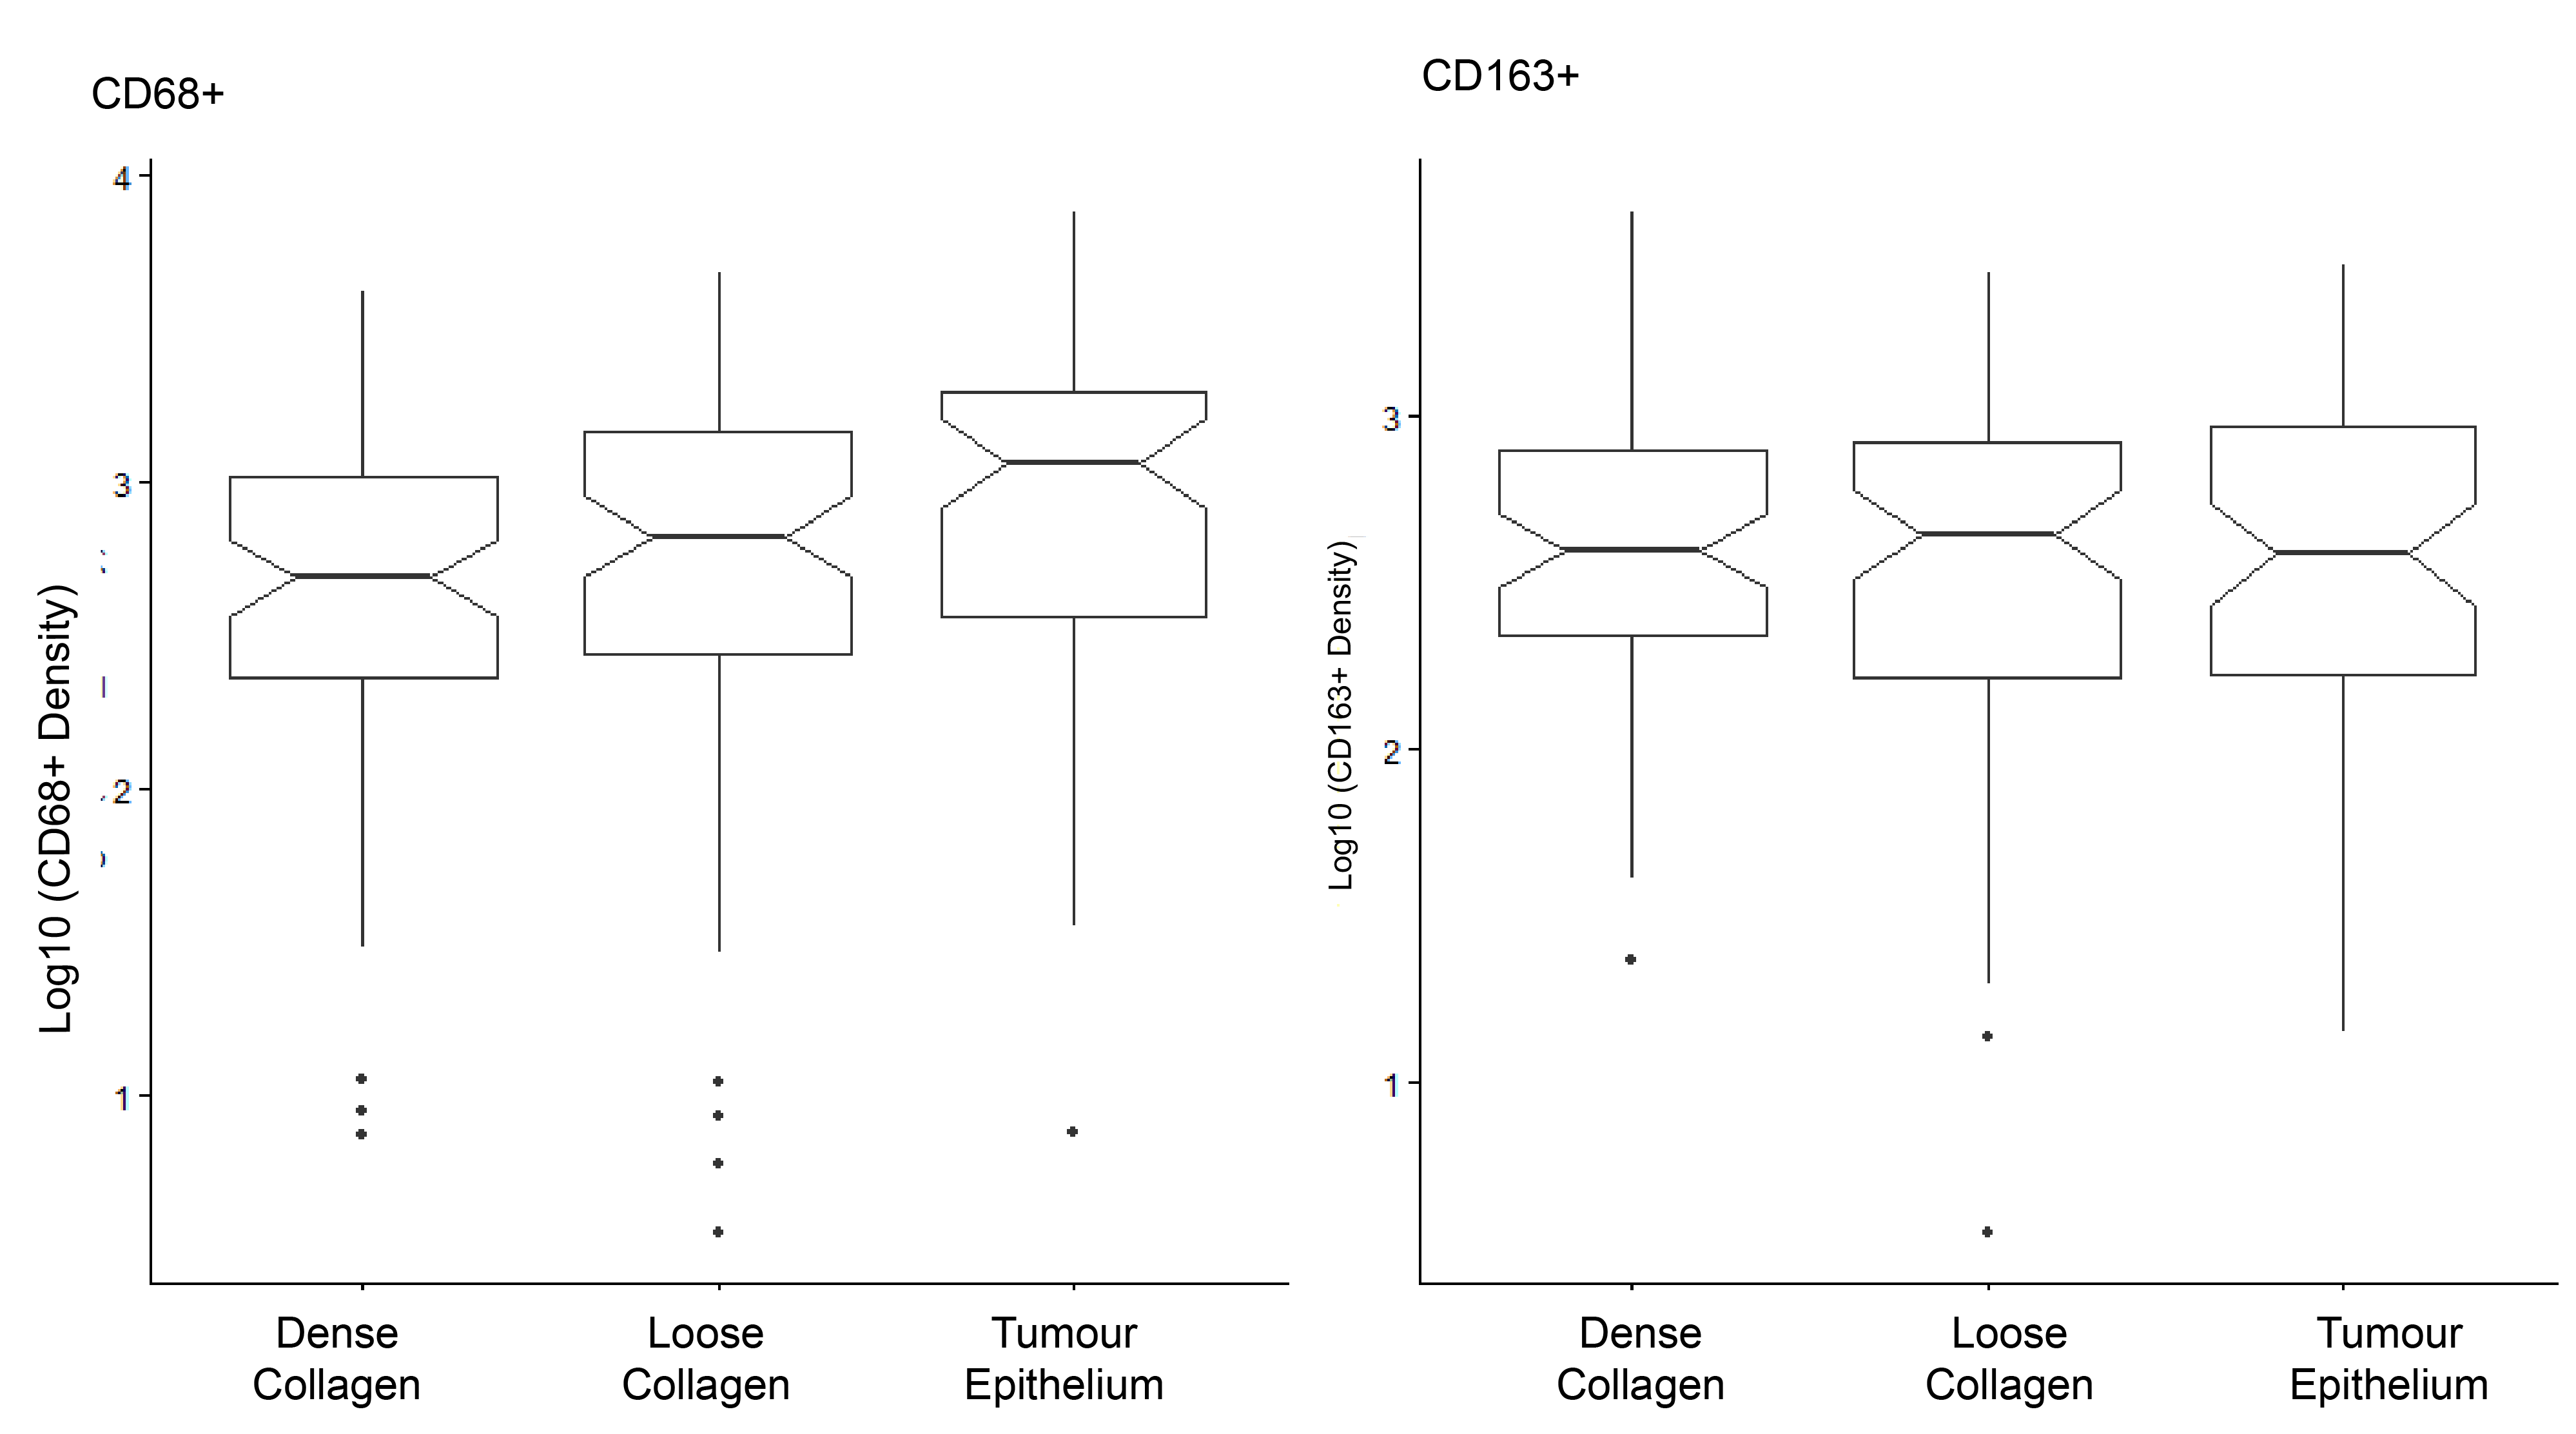
\includegraphics[width=0.9\textwidth]{Chapter4/figs/Thesis-10.png}
    \caption{Distribution of densities of CD68+ and CD163+ cells in the dense collagen, loose collagen and epithelial regions of the tumour section.}
    \label{fig:distribution}
\end{figure}

The area density of the immune infiltrates does not vary between, given that the nuclear 

\subsection{Collagen structure analysis}

\section{Discussion}
The ability to measure collagen deposition, patterns of immune infiltration and hypoxia simultaneously on one slide have led to a much more in depth and concrete results on the intersection between these.
Survival analysis showed that. 


%\include{Chapter5/chapter5}
%\include{Chapter6/chapter6}
%\include{Chapter7/chapter7}



% ********************************** Back Matter *******************************
% Backmatter should be commented out, if you are using appendices after References
%\backmatter

% ********************************** Bibliography ******************************
\begin{spacing}{0.9}

% To use the conventional natbib style referencing
% Bibliography style previews: http://nodonn.tipido.net/bibstyle.php
% Reference styles: http://sites.stat.psu.edu/~surajit/present/bib.htm

\bibliographystyle{apalike}
%\bibliographystyle{unsrt} % Use for unsorted references  
%\bibliographystyle{plainnat} % use this to have URLs listed in References
\cleardoublepage
%\bibliography{References/references} % Path to your References.bib file
\bibliography{References/references2}

% If you would like to use BibLaTeX for your references, pass `custombib' as
% an option in the document class. The location of 'reference.bib' should be
% specified in the preamble.tex file in the custombib section.
% Comment out the lines related to natbib above and uncomment the following line.

%\printbibliography[heading=bibintoc, title={References}]


\end{spacing}

% ********************************** Appendices ********************************

\begin{appendices} % Using appendices environment for more functionality


%!TEX root = ../thesis.tex
% ******************************* Thesis Appendix A ********************************

\chapter{Probability Density}
 The probability density function is the function that gives the probability of a particular value occurring. $P(x)=f(x)$
 
And the equivalent form that all probabilities sum to 1 is the following equation:
\begin{equation}
    \int_{-\infty}^{\infty}f(x)dx = 1
\end{equation}

The expected or mean value of x is 
\begin{equation}
   \bar{x}= \int_{-\infty}^{\infty}xf(x)dx
\end{equation}

In 2D when we analyse a point distribution with a constant probability of a point occurring, the point density $k$, the probability density function is the following;

\begin{equation}
  f(r)=k
\end{equation}

When we integrate this in radial coordinates over a circular area with radius $R$;
\begin{equation}
  \int_0^\infty k.2\pi r.dr = \int_0^R k.2\pi r.dr = 1
\end{equation}

\begin{equation}
k. \pi R^2 = 1 
\end{equation}

\begin{equation}
    k=\frac{1}{\pi R^2}
\end{equation}
The probability $k$ of finding a point at radius, $r$, is $\frac{1}{\pi R^2}$. 
The probability of finding $N$ points is $\frac{N}{\pi R^2}$

Therefore the probability of finding a point between $r$ and $r + dr$ is
\begin{equation}
    $\frac{2 \pi}{\pi R^2} dr$
\end{equation}
% ******************************* Thesis Appendix A ********************************

\chapter{Supplementary Figures}
\section{Sequencing Depth and Allele Frequency of technical replicates}
\begin{figure}
    \centering
    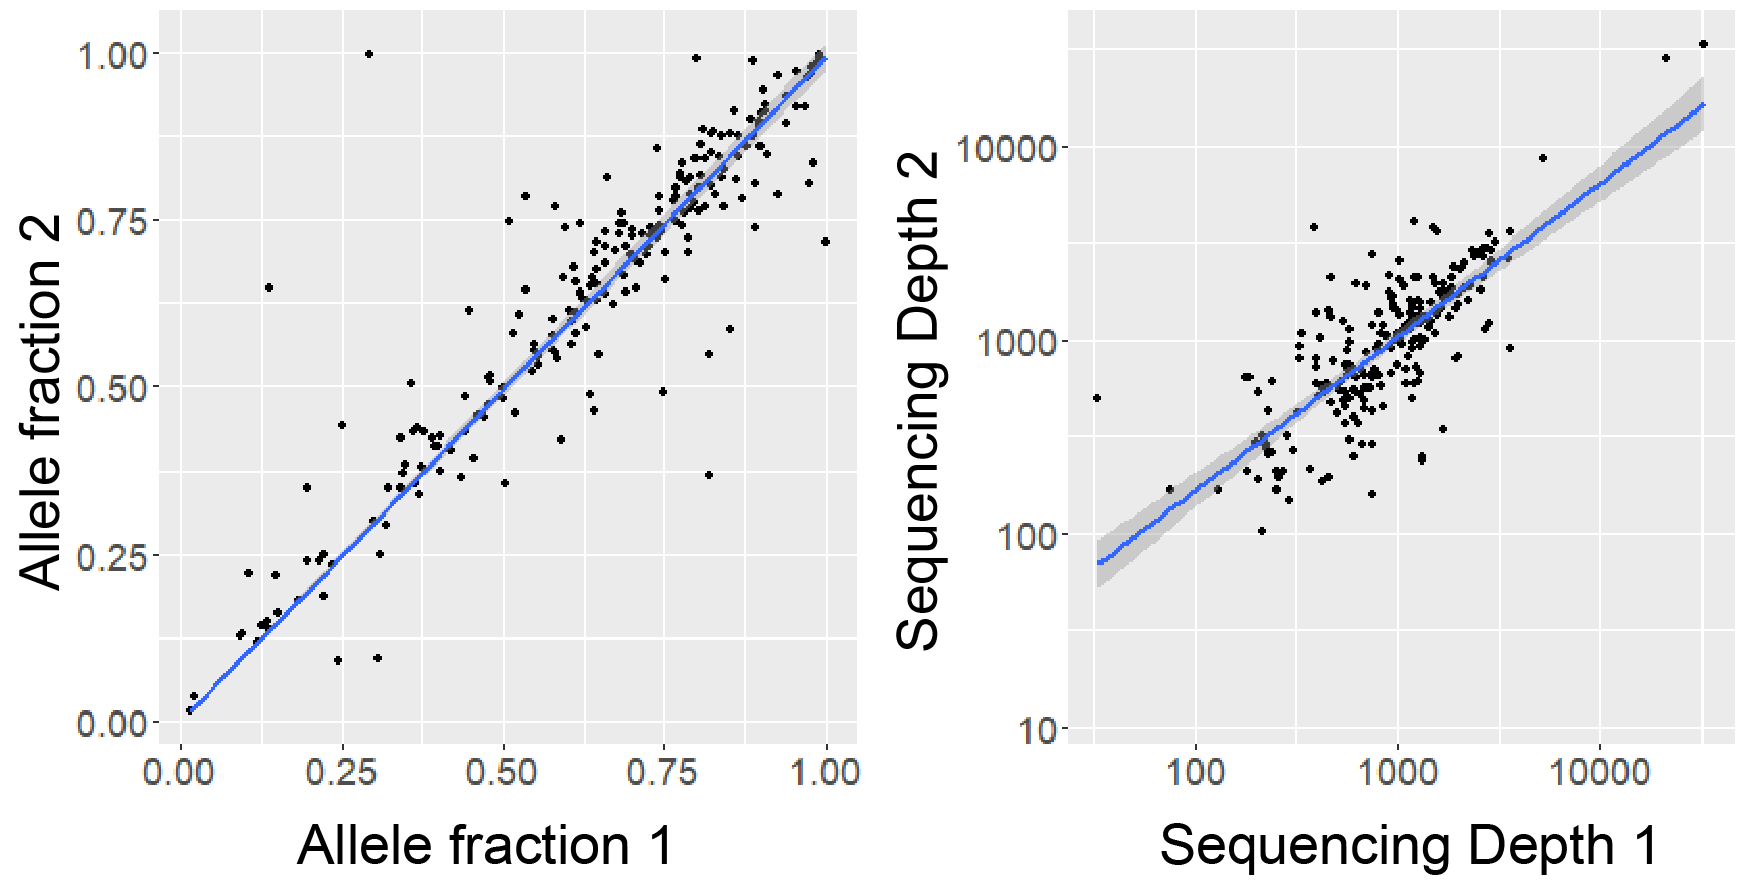
\includegraphics{Chapter2/Figs/Raster/p53_allele.png}
    \caption{\textit{p53} allele fraction and sequencing depth for technical replicates.}
    \label{fig:p53_allele}
\end{figure}

\end{appendices}

% *************************************** Index ********************************
\printthesisindex % If index is present

\end{document}
